% Chapter 5 — Sheaves, Cohomology, and the de Rham Theorem (reviewed)
\chapter{Sheaves, Cohomology, and the de Rham Theorem}

SHEAVES,

COHOMOLOGY,

and the DE RHAM THEOREM

The principal objective in this chapter is a proof of the de Rham theorem, one version of which we have stated in 4.17. In its most complete form it asserts that the homomorphism from the de Rham cohomology ring to the differentiable singular cohomology ring given by integration of closed forms over differentiable singular cycles is a ring isomorphism. The approach will be to exhibit both the de Rham cohomology and the differentiable singular cohomology as special cases of sheaf cohomology and to use a basic uniqueness theorem for homomorphisms of sheaf cohomology theories to prove that the natural homomorphism between the de Rham and differentiable singular theories is an isomorphism. As an added dividend of this approach we shall also obtain the existence of canonical isomorphisms of the de Rham and differentiable singular cohomology theories with the continuous singular theory, the Alexander-Spanier theory, and the Czech cohomology theory for differentiable manifolds. From these isomorphisms we shall conclude that the de Rham cohomology theory is a topological invariant of a differentiable manifold.

No previous knowledge of sheaf theory nor of any of these cohomology theories is assumed. We shall develop those aspects of the theories necessary for our applications. We begin with an introduction to the theory of sheaves and sheaf cohomology. Our approach is based largely on the development given by Cartan in [4]. The interested reader will find more general treatments of sheaf theory in Cartan [4], Godement [7], and Bredon [3]. Sheaves are a very powerful tool in the study of complex manifolds. For an excellent account of their use in the theory of Riemann surfaces, see Gunning [8].

Let M be a differentiable manifold. Recall that M is assumed to be second countable and is therefore paracompact. It should be pointed out that nearly all of the sheaf theory presented in this chapter depends only on M being a paracompact Hausdorff space. The differentiable structure on M will be invoked only in a few examples and in the discussions of the Rham cohomology (5.28) and the differentiable singular cohomology (5.31); and, in addition, the locally Euclidean structure will be invoked in the discussion of the singular cohomology (5.31). Otherwise, M need only be a paracompact Hausdorff space.

Throughout this chapter, K will be a fixed principal ideal domain. We shall treat sheaves of K-modules over M. The most important cases to keep in mind are these: \index{K-modules}

(i) K is the ring of integers Z, whence a K-module is simply an abelian group.

(ii) K is the field of real numbers  $ \mathbb{R} $, whence a K-module is simply a real vector space.

For the first few sections of this chapter, K could be any ring. The additional property that K is a principal ideal domain will be used first in 5.13.

\section{Sheaves and Presheaves}


\begin{definition}\label{thm:5.1}
A sheaf $\mathcal{S}$ of $K$-modules over $M$ consists of a topological space $\mathcal{S}$ together with a map $\pi\colon \mathcal{S} \to M$ satisfying:

(a)  $ \pi $ is a local homeomorphism of S onto  $ M $.

(b)  $ \pi^{-1}(m) $ is a K-module for each  $ m \in M $.

(c) The composition laws are continuous in the topology on S.

We elaborate on (c). Let $\mathcal{S}\circ\mathcal{S}$ be the subspace of $\mathcal{S}\times\mathcal{S}$ consisting of all pairs $(s_1,s_2)$ such that $\pi(s_1)=\pi(s_2)$. Then (c) requires that the map $(s_1,s_2)\mapsto s_1-s_2$ of $\mathcal{S}\circ\mathcal{S}\to\mathcal{S}$ be continuous, and that each of the maps $s\mapsto k s$ of $\mathcal{S}\to\mathcal{S}$ for $k\in K$ be continuous. It follows easily that the maps $s\mapsto(-s)$ and $(s_1,s_2)\mapsto s_1+s_2$ also are continuous. Sheaves of $K$ algebras are defined similarly, with the additional requirement in (c) that the map $(s_1,s_2)\mapsto s_1\cdot s_2$ of $\mathcal{S}\circ\mathcal{S}\to\mathcal{S}$ be continuous.

The map $\pi$ is called the projection; and the $K$-module $\mathcal{S}_m = \pi^{-1}(m)$ is called the stalk over $m \in M$. Let $U \subset M$ be open. A continuous map $f: U \to \mathcal{S}$ such that $\pi \circ f = id$ is called a section of $\mathcal{S}$ over $U$. The 0-section is the section which associates with $m \in U$ the zero element of $\mathcal{S}_m$. We let $\Gamma(\mathcal{S}, U)$ denote the set of sections of $\mathcal{S}$ over $U$. We make $\Gamma(\mathcal{S}, U)$ into a $K$-module as follows. Let $f$ and $g$ belong to $\Gamma(\mathcal{S}, U)$, and let $k \in K$. We define the sum of $f$ and $g$ to be the section

\[
(f+g)(m)=f(m)+g(m)\qquad(m\in U),
\]

and we define a section $kf$ by setting

\[
(k f)(m)=k\bigl(f(m)\bigr)\qquad(m\in U).
\]

With these operations, $\Gamma(\mathcal{S},U)$ becomes a $K$-module. The module of sections of $\mathcal{S}$ over $M$ (global sections) will simply be denoted by $\Gamma(\mathcal{S})$. Observe that since $\pi$ is a local homeomorphism, sections are open maps; and if sections $f$ and $g$ agree at $m\in M$, then they must agree on a neighborhood of $m$.

\end{definition}

\begin{examples}\label{thm:5.2}
The most elementary example of a sheaf over $M$ is that of a so-called constant sheaf $\mathcal{G} = M \times G$, where $G$ is a $K$-module with the discrete topology and $\mathcal{G}$ is given the product topology. Here the projection is simply $\pi(m,g) = m$. \index{Constant sheaf}

A less trivial example is the following. Let $\bar{F}_{m}$ denote the set of germs of $C^{\infty}$ functions at $m\in M$ (as in 1.13), and let

\begin{equation}
\label{eq:5.2:1}
\mathcal{C}^{\infty}(M)=\bigcup_{m\in M}\bar{F}_{m}.
\end{equation}

When it will introduce no confusion, we shall denote $\mathcal{C}^{\infty}(M)$ simply by $\mathcal{C}^{\infty}$. We define the projection $\pi\colon \mathcal{C}^{\infty} \to M$ in the obvious fashion so that $f \in \bar{F}_{\pi(f)}$. Associate with each open set $U$ in $M$ and each $C^{\infty}$ function $f$ on $U$ the set

\[
\bigcup_{m\in U}f_{m}\subset\mathcal{C}^{\infty},
\]

where  $ f_m $ is the germ of  $ f $ at  $ m $. The collection of these sets forms a basis for a topology on  $ \mathcal{C}^\infty $ which makes  $ \mathcal{C}^\infty $ into a sheaf of real vector spaces (in fact, a sheaf of algebras since each  $ \bar{F}_m $ has an algebra structure).  $ \mathcal{C}^\infty(M) $ is called the sheaf of germs of  $ C^\infty $ functions on  $ M $. Similarly, one constructs the sheaf  $ \mathcal{C}^p(M) $ of germs of functions of class  $ C^p $ on  $ M $ for each integer  $ p \geq 0 $. \index{Sheaf}

\end{examples}

\begin{remarks}\label{thm:5.3}
One should be cautioned that sheaves are generally not Hausdorff spaces. A simple example is provided by the sheaf  $ \mathcal{C}^0(\mathbb{R}) $ of germs of continuous functions on the real line. Let  $ g(t) \equiv 0 $, let  $ f(t) = 0 $ for  $ t \leq 0 $, and let  $ f(t) = t $ for  $ t > 0 $. Then the germs of  $ f $ and  $ g $ at the origin are distinct elements of  $ \mathcal{C}^0(\mathbb{R}) $; however,  $ f $ and  $ g $ have the same germ for each  $ t < 0 $. It follows that the germs of  $ f $ and  $ g $ at the origin cannot be separated by disjoint open sets in  $ \mathcal{C}^0(\mathbb{R}) $.

\end{remarks}

\begin{definition}\label{thm:5.4}
Let $\mathcal{S}$ and $\mathcal{S}'$ be sheaves on $M$ with projections $\pi$ and $\pi'$ respectively. A continuous map $\varphi\colon \mathcal{S} \to \mathcal{S}'$ such that  $ \pi' \circ \varphi = \pi $ is called a sheaf mapping. Observe that sheaf mappings are necessarily local homeomorphisms, and they map stalks into stalks. A sheaf mapping  $ \varphi $ which is a homomorphism (of K-modules) on each stalk is called a sheaf homomorphism. A sheaf isomorphism is a sheaf homomorphism with an inverse which is also a sheaf homomorphism.

An open set $\mathcal{R}$ in the sheaf $\mathcal{S}$ such that the subset $\mathcal{R}_m = \mathcal{R} \cap \mathcal{S}_m$ is a submodule of $\mathcal{S}_m$ for each $m \in M$ is called a subsheaf of $\mathcal{S}$. It is clear that a subsheaf of $\mathcal{S}$, with the natural topology and the projection map which it inherits from $\mathcal{S}$, is again a sheaf.

Let $\varphi: \mathcal{S} \to \mathcal{T}$ be a homomorphism of sheaves. The kernel of $\varphi$ (ker $\varphi$) is the subset of $\mathcal{S}$ which maps under $\varphi$ into the 0-section of $\mathcal{T}$, and is in fact a subsheaf of $\mathcal{S}$. The subsheaf $\varphi(\mathcal{S}) \subset \mathcal{T}$ is called the image of $\varphi$ (im $\varphi$). In the case in which $\varphi$ is one-to-one, we shall often identify $\mathcal{S}$ with $\varphi(\mathcal{S})$ and speak of the subsheaf $\mathcal{S}$ of $\mathcal{T}$.

Let $\mathcal{R}$ be a subsheaf of $\mathcal{S}$. For each $m\in M$, let $\mathcal{T}_{m}$ denote the quotient module $\mathcal{S}_{m}/\mathcal{R}_{m}$, and let

\begin{equation}
\label{eq:5.4:1}
\mathcal{T}=\bigcup_{m\in M}\mathcal{T}_{m}.
\end{equation}

Let $\tau: \mathcal{S} \to \mathcal{T}$ be the natural map which associates with each element of $\mathcal{S}_m$ its coset in $\mathcal{T}_m$, for each $m$, and give $\mathcal{T}$ the quotient topology. That is, a set $U$ in $\mathcal{T}$ will be open if and only if $\tau^{-1}(U)$ is open in $\mathcal{S}$. Then, with this topology and with the natural projection which maps each element of $\mathcal{T}_m$ to $m$, $\mathcal{T}$ is a sheaf over $M$ and $\tau: \mathcal{S} \to \mathcal{T}$ is a sheaf homomorphism. We leave the details as an exercise. $\mathcal{T}$ is called the quotient sheaf of $\mathcal{S}$ modulo $\mathcal{R}$. \index{Quotient sheaf}

If $\varphi: \mathcal{S} \to \mathcal{T}$ is a homomorphism of sheaves, then it is easily checked that the natural map $\mathcal{S}/\ker \varphi \to \mathrm{im} \varphi$ given by $(s + (\ker \varphi \mid \mathcal{S}_m)) \mapsto \varphi(s)$ for $s \in \mathcal{S}_m$ is a sheaf isomorphism.

A sequence of sheaves and homomorphisms

\begin{equation}
\label{eq:5.4:2}
\cdots\to\mathcal{S}_{i}\to\mathcal{S}_{i+1}\to\mathcal{S}_{i+2}\to\cdots
\end{equation}

is called exact if at each stage the image of a given homomorphism is the kernel of the next. Exact sequences of K-modules are defined similarly. Observe that (2) is exact if and only if for each $m\in M$ the induced sequence of homomorphisms of the stalks over $m$, namely,

\begin{equation}
\label{eq:5.4:3}
\cdots\to(\mathcal{S}_{i})_{m}\to(\mathcal{S}_{i+1})_{m}\to(\mathcal{S}_{i+2})_{m}\to\cdots,
\end{equation}

is exact. If $\mathcal{R}$ is a subsheaf of $\mathcal{S}$, and $\mathcal{T}$ is the quotient sheaf $\mathcal{S}/\mathcal{R}$, then the natural sequence of homomorphisms

\begin{equation}
\label{eq:5.4:4}
0\to\mathcal{R}\to\mathcal{S}\to\mathcal{T}\to0
\end{equation}

is exact, where 0 denotes the constant sheaf over M whose stalk over each point is the trivial K-module consisting of only one element. Exact sequences of the form (4) consisting of only five terms with the first and last being the 0 sheaf are called short exact sequences. Short exact sequences of K-modules are defined similarly.

\end{definition}

\subsection{Presheaves}\label{thm:5.5} A presheaf $P = \{S_U; \rho_{U,V}\}$ of $K$-modules on $M$ consists of a $K$-module $S_U$ for each open set $U$ in $M$ and a homomorphism $\rho_{U,V}: S_V \to S_U$ for each inclusion $U \subset V$ of open sets in $M$, such that $\rho_{U,U} = \mathrm{id}$, and such that whenever $U \subset V \subset W$, the following diagram commutes: \index{Presheaf}

\begin{equation}
\label{eq:5.5:1}
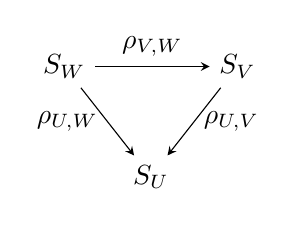
\begin{tikzpicture}[baseline={(current bounding box.center)},>=stealth]
\node (SW) at (0,1.4) {$S_W$};
\node (SV) at (2.2,1.4) {$S_V$};
\node (SU) at (1.1,0) {$S_U$};
\draw[->] (SW) -- node[above] {$\rho_{V,W}$} (SV);
\draw[->] (SW) -- node[left] {$\rho_{U,W}$} (SU);
\draw[->] (SV) -- node[right] {$\rho_{U,V}$} (SU);
\end{tikzpicture}
\end{equation}

A typical example of a presheaf is the following. Associate with each open set $U$ in $M$ the algebra $C^\infty(U)$ of $C^\infty$ functions on $U$, and let $\rho_{U,V}$ be the map which restricts a $C^\infty$ function on $V$ to a $C^\infty$ function on $U$. This yields a presheaf $\{C^\infty(U);\rho_{U,V}\}$ of real vector spaces (in fact algebras) on $M$. Similarly, one could associate with $U$ the vector space of $p$-forms on $U$ for some fixed $p$ and again let $\rho_{U,V}$ be the restriction mapping.

Let $P=\{S_{U};\rho_{U,V}\}$ and $P^{\prime}=\{S_{U}^{\prime};\rho_{U,V}^{\prime}\}$ be presheaves on $M$. By a presheaf homomorphism of $P$ to $P^{\prime}$ we mean a collection $\{\varphi_{U}\}$ of homomorphisms $\varphi_{U}\colon S_{U}\to S_{U}^{\prime}$ such that

\begin{equation}
\label{eq:5.5:2}
\rho_{U,V}^{\prime}\circ\varphi_{V}=\varphi_{U}\circ\rho_{U,V}
\end{equation}

whenever $U \subset V$. A presheaf isomorphism is a presheaf homomorphism $\{\varphi_{U}\}$ in which each $\varphi_{U}$ is an isomorphism of $K$-modules.

\subsection{The Relationship between Sheaves and Presheaves}\label{thm:5.6} Each sheaf  $ \mathcal{S} $ gives rise canonically to a presheaf  $ \{\Gamma(\mathcal{S},U);\rho_{U,V}\} $. Here we associate with each open set  $ U $ in  $ M $ the  $ K $-module  $ \Gamma(\mathcal{S},U) $ of sections of  $ \mathcal{S} $ over  $ U $, and to each inclusion  $ U \subset V $ of open sets in  $ M $ we associate the homomorphism

\begin{equation}
\label{eq:5.6:1}
\rho_{U,V}\colon\Gamma(\mathcal{S},V)\to\Gamma(\mathcal{S},U)
\end{equation}

which maps a section of $\mathcal{S}$ over $V$ to its restriction to U. We shall denote this map of sheaves to presheaves by $\alpha$. We call $\alpha(\mathcal{S})$ the presheaf of sections of the sheaf $\mathcal{S}$.

Conversely, we shall now show that each presheaf canonically determines a sheaf, which we call its associated sheaf. In practice, many sheaves will in this manner arise naturally from presheaves. The best example to keep in mind during the following construction is the presheaf  $ \{C^\infty(U);\rho_{U,V}\} $; its associated sheaf will be the sheaf of germs of  $ C^\infty $ functions on  $ M $.

Let $P = \{S_U; \rho_{U,V}\}$ be a presheaf of $K$-modules on $M$. Let $m \in M$, and let $S_m^*$ be the disjoint union of each of the modules $S_U$ for which $m \in U$. If we set $f \in S_U$ equivalent to $g \in S_V$ if and only if there is a neighborhood $W$ of $m$ with $W \subset U \cap V$ such that $\rho_{W,U}f = \rho_{W,V}g$, we obtain an equivalence relation on $S_m^*$. The set $S_m$ of equivalence classes of elements of $S_m^*$ will be the stalk of the associated sheaf over $m$. If $m \in U$, let $\rho_{m,U}: S_U \to S_m$ be the natural projection which assigns to each element of $S_U$ its equivalence class. Let $f \in S_U$ and $g \in S_V$ be representatives of classes $s_1$ and $s_2$ in $S_m$ respectively. There exists a neighborhood $W$ of $m$ such that $W \subset U \cap V$. Define addition in $S_m$ by setting

\begin{equation}
\label{eq:5.6:3}
s_{1}+s_{2}=\rho_{m,w}(\rho_{W,U}f+\rho_{W,V}g),
\end{equation}

and define multiplication by  $ k \in K $ by setting

\begin{equation}
\label{eq:5.6:4}
k s_{1}=\rho_{m,U}(k f).
\end{equation}

It is easy to check that the operations in (3) and (4) are well-defined and give $S_{m}$ the structure of a $K$-module such that the maps $\rho_{m,U}$ are all homomorphisms. $S_{m}$ is known as the direct limit of the modules $S_{U}$ for $U$ containing $m$. Now let \index{Direct limit of K-modules}

\begin{equation}
\label{eq:5.6:5}
\mathcal{S}=\bigcup_{m\in M}\mathcal{S}_{m},
\end{equation}

and let $\pi: \mathcal{S} \to M$ be the obvious projection such that $\pi(\mathcal{S}_m) = m$. We topologize $\mathcal{S}$ by taking for a basis of the topology the collection of subsets of $\mathcal{S}$ of the form

\begin{equation}
\label{eq:5.6:6}
O_{f}=\{\rho_{p,U}f\colon p\in U\}
\end{equation}

for the various $f\in S_U$ and the various open sets $U$ in $M$. This collection does indeed form a basis for a topology on $\mathcal{S}$, for if $s\in O_f\cap O_g$, say $s=\rho_{p,U}f=\rho_{p,V}g$, then there is a neighborhood $W$ of $p$ with $W\subset U\cap V$ for which $\rho_{W,U}f=\rho_{W,V}g$, from which it follows that $s\in O_{\rho_{W,U}f}\subset O_f\cap O_g$.

We claim that $\mathcal{S}$ is a sheaf over $M$ with projection $\pi$. Now $\pi$ is a local homeomorphism since it is a homeomorphism on each $O_f$. Each stalk $\mathcal{S}_m$ has been given the structure of a $K$-module, so finally we need only check that the composition operations are continuous. Consider first multiplication by $k \in K$. Let $s \in \mathcal{S}$, and let $O$ be an open neighborhood of $ks$. Let $s = \rho_{p,U}f$. Then $O_{k f}$ is also an open neighborhood of $ks$. Let $V$ be a neighborhood of $p$ contained in $\pi(O_{k f} \cap O)$. Then $O_{\rho_{V,U}f}$ is an open neighborhood of $s$ which maps under multiplication by $k$ into the open neighborhood $O_{\rho_{V,U}kf} \subset O$ of $ks$. Finally, we show that the map $(s_1, s_2) \mapsto s_1 - s_2$ of $\mathcal{S} \circ \mathcal{S} \to \mathcal{S}$ is continuous. For let $O_f$ be an open neighborhood of $s_1 - s_2$, say $s_1 - s_2 = \rho_{p,U}f$, and let $s_1 = \rho_{p,V}g$ and $s_2 = \rho_{p,W}h$. Then there exists an open neighborhood $Q$ of $p$ with $Q \subset U \cap V \cap W$ such that

\begin{equation}
\label{eq:5.6:7}
\rho_{Q,U}f=\rho_{Q,V}g-\rho_{Q,W}h.
\end{equation}

It follows that the open neighborhood

\begin{equation}
\label{eq:5.6:8}
O_{\rho_{Q,V}g}\times O_{\rho_{Q,W}h}\cap\mathcal{S}\circ\mathcal{S}
\end{equation}

of $(s_{1}, s_{2})$ maps into $O_{f}$. Thus the composition operations are continuous, and $\mathcal{S}$ is a sheaf over $M$ with projection $\pi$. $\mathcal{S}$ is called the sheaf associated with the presheaf $P$. We shall denote this map of presheaves to sheaves by $\beta$; thus $\mathcal{S} = \beta(P)$.

Clearly, each sheaf homomorphism $\varphi\colon\mathcal{S}\to\mathcal{T}$ gives rise to a presheaf homomorphism between the presheaves of sections $\alpha(\mathcal{S})$ and $\alpha(\mathcal{T})$ by composing elements of $\Gamma(\mathcal{S},U)$ with $\varphi$. Conversely, a presheaf homomorphism $\{\varphi_U\}$ from $P$ to $P'$ canonically induces a homomorphism $\varphi$ of the associated sheaves $\beta(P)$ and $\beta(P')$ such that

\begin{equation}
\label{eq:5.6:9}
\rho_{p,U}^{\prime}\circ\varphi_{U}=\varphi\circ\rho_{p,U}
\end{equation}

for each open set $U$ in $M$ and each $p \in U$. Moreover, in going in either direction, from homomorphisms of sheaves to homomorphisms of presheaves, or vice versa, the composition of two homomorphisms induces the composition of the corresponding homomorphisms.

Suppose now that we start with a sheaf $\mathcal{S}$, take its presheaf $\alpha(\mathcal{S})$ of sections, and then form the associated sheaf $\beta(\alpha(\mathcal{S}))$, thus obtaining the sheaf of germs of sections of $\mathcal{S}$. Then the sheaves $\mathcal{S}$ and $\beta(\alpha(\mathcal{S}))$ are canonically isomorphic. Indeed, let $\xi \in \beta(\alpha(\mathcal{S}))$ be the germ at $p$ of some section $f$ of $\mathcal{S}$ over an open set $U$ containing $p$; that is, $\xi = \rho_{p,U}f$ for $f \in \Gamma(\mathcal{S}, U)$. Then $\xi \mapsto f(p)$ determines a well-defined map $\beta(\alpha(\mathcal{S})) \to \mathcal{S}$ which is a sheaf isomorphism. We leave the details as an exercise.

Generally, however, if we start with a presheaf $P$ and take the presheaf $\alpha(\beta(P))$ of sections of the sheaf associated with $P$, we may get a presheaf quite distinct from $P$. For example, let $P = \{S_U; \rho_{U,V}\}$ where $S_U$ is the principal ideal domain $K$ for each $U$, and all restrictions $\rho_{U,V}$ for $U \subsetneq V$ are identically 0. Then the presheaf $\alpha(\beta(P))$ assigns to each open set $U$ in $M$ the zero $K$-module. The conditions of the following definition are clearly necessary if $P$ is to be isomorphic with $\alpha(\beta(P))$, and it will be shown in §5.8 that they are also sufficient.

\begin{definition}\label{thm:5.7}
A presheaf $\{S_{U};\rho_{U,V}\}$ on $M$ is said to be complete if whenever the open set $U$ is expressed as a union $\bigcup U_{\alpha}$ of open sets in $M$, the following two conditions are satisfied:

$(C_{1})'$ Whenever $f$ and $g$ in $S_{U}$ are such that $\rho_{U_{\alpha},U}f = \rho_{U_{\alpha},U}g$ for all $\alpha$, then $f = g$.

$(C_{2})$ Whenever there is an element $f_{\alpha}\in S_{U_{\alpha}}$ for each $\alpha$ such that $\rho_{U_{\alpha}\cap U_{\beta},U_{\alpha}}f_{\alpha}=\rho_{U_{\alpha}\cap U_{\beta},U_{\beta}}f_{\beta}$ for all $\alpha$ and $\beta$, then there exists $f\in S_{U}$ such that $f_{\alpha}=\rho_{U_{\alpha},U}f$ for each $\alpha$.

\end{definition}

\begin{proposition}\label{thm:5.8}
If $P$ is a complete presheaf, then $\alpha(\beta(P))$ is canonically isomorphic with $P$.

\end{proposition}

\begin{proof}
Let $P=\{S_{U};\rho_{U,V}\}$. We define a presheaf homomorphism from $P$ to $\alpha(\beta(P))$ as follows. For each open set $U$ in $M$ we map

\begin{equation}
\label{eq:5.8:1}
S_{U}\to\Gamma\bigl(\beta(P),U\bigr)
\end{equation}

by sending the element f of  $ S_{U} $ to the section

\begin{equation}
\label{eq:5.8:2}
p\mapsto\rho_{p,U}f
\end{equation}

of $\beta(P)$ over $U$. To prove that this presheaf homomorphism is an isomorphism, we need to prove that each of the homomorphisms (1) are isomorphisms. Injectivity follows from $5.7(C_{1})$, for if $f$ in $S_{U}$ maps to the 0-section, then there exists a cover $\{U_{\alpha}\}$ of $U$ such that $\rho_{U_{\alpha},U}f=\rho_{U_{\alpha},U}(0)$. Therefore $f=0\in S_{U}$ by $(C_{1})$. To prove surjectivity, let $c$

be a section of $\beta(P)$ over $U$. Then for each $p \in U$, there is a neighborhood $U_p$ of $p$ and an element $f_p \in S_{U_p}$ such that

\begin{equation}
\label{eq:5.8:3}
\rho_{q,U_{p}}f_{p}=c(q)
\end{equation}

for all $q\in U_{p}$. It follows from (3) and $5.7(C_{1})$ that for each $p$ and $q$ in $U$,

\begin{equation}
\label{eq:5.8:4}
\rho_{U_{p}\cap U_{q},U_{p}}f_{p}=\rho_{U_{p}\cap U_{q},U_{q}}f_{q}.
\end{equation}

Thus, according to 5.7($C_{2}$), there exists $f \in S_{U}$ such that

\begin{equation}
\label{eq:5.8:5}
f_{p}=\rho_{U_{p},U}f
\end{equation}

for each $p \in U$. It follows from (5), (3), and (2) that $f$ maps to $c$ under the homomorphism (1).

\end{proof}

\subsection{Tensor Products}\label{thm:5.9} Before we define the tensor products of sheaves and presheaves, we need a few preliminary remarks. The definition of the tensor product  $ S \otimes T $ of K-modules S and T is completely analogous to that for the special case 2.1 of tensor products of $R$-modules. If  $ f: S \to S' $ and  $ h: T \to T' $ are homomorphisms of K-modules, then their tensor product  $ f \otimes h $ is the homomorphism of  $ S \otimes T $ into  $ S' \otimes T' $ uniquely associated by the universal mapping property \hyperref[thm:2.2]{2.2(a)} with the bilinear map

\begin{equation}
\label{eq:5.9:1}
(s,t)\mapsto f(s)\otimes h(t)
\end{equation}

of  $ S \times T $ into  $ S' \otimes T' $.

Observe that if S is a K-module, then there is a canonical isomorphism

\begin{equation}
\label{eq:5.9:2}
S\otimes K\cong S.
\end{equation}

Indeed, let $f: S \otimes K \to S$ be the homomorphism determined by the bilinear map $(s, k) \mapsto ks$ of $S \times K \to S$. Then $f$ is clearly surjective, and is also injective since $\sum_{i}(s_{i} \otimes k_{i}) = \left(\sum_{i} k_{i} s_{i}\right) \otimes 1$, so if $f\left(\sum_{i}(s_{i} \otimes k_{i})\right) = 0$, then $\sum_{i} k_{i} s_{i} = 0$, which implies $\sum_{i}(s_{i} \otimes k_{i}) = 0$.

Now let $P=\{S_{U};\rho_{U,V}\}$ and $P^{\prime}=\{S_{U}^{\prime};\rho_{U,V}^{\prime}\}$ be presheaves on $M$. Then their tensor product is the presheaf

\begin{equation}
\label{eq:5.9:3}
\begin{array}{r}{P\otimes P^{\prime}=\{S_{U}\otimes S_{U}^{\prime};\rho_{U,V}\otimes\rho_{U,V}^{\prime}\}.}\end{array}
\end{equation}

If $\{\varphi_U\}$: $P \to Q$ and $\{\varphi'_U\}$: $P' \to Q'$ are homomorphisms of presheaves (\eqref{eq:5.5:2}), then their tensor product $\{\varphi_U\} \otimes \{\varphi'_U\}$ is by definition the homomorphism $\{\varphi_U \otimes \varphi'_U\}$ of $P \otimes P'$ into $Q \otimes Q'$.

If $\mathcal{S}$ and $\mathcal{T}$ are sheaves over $M$, we define their tensor product $\mathcal{S} \otimes \mathcal{T}$ to be the sheaf associated with the tensor product of the presheaves of sections of $\mathcal{S}$ and $\mathcal{T}$. That is,

\begin{equation}
\label{eq:5.9:4}
\mathcal{S}\otimes\mathcal{T}=\beta\big(\alpha(\mathcal{S})\otimes\alpha(\mathcal{T})\big).
\end{equation}

Moreover, if $\varphi: \mathcal{S} \to \mathcal{T}$ and $\gamma: \mathcal{S}' \to \mathcal{T}'$ are sheaf homomorphisms, and if $\{\varphi_U\}: \alpha(\mathcal{S}) \to \alpha(\mathcal{T})$ and $\{\gamma_U\}: \alpha(\mathcal{S}') \to \alpha(\mathcal{T}')$ are the corresponding homomorphisms on the presheaves of sections, then we define the tensor product $\varphi \otimes \gamma$ to be the homomorphism $\mathcal{S} \otimes \mathcal{S}' \to \mathcal{T} \otimes \mathcal{T}'$ associated with the presheaf homomorphism

\begin{equation}
\label{eq:5.9:5}
\{\varphi_{U}\}\otimes\{\gamma_{U}\}\colon\alpha(\mathcal{S})\otimes\alpha(\mathcal{S}^{\prime})\to\alpha(\mathcal{T})\otimes\alpha(\mathcal{T}^{\prime}).
\end{equation}

The reader should check that there is a canonical isomorphism

\begin{equation}
\label{eq:5.9:6}
(\mathcal{S}\otimes\mathcal{T})_{m}\cong\mathcal{S}_{m}\otimes\mathcal{T}_{m},
\end{equation}

so in particular if $\mathcal{K}$ is the constant sheaf $M\times K$, then in view of (2) there is a canonical isomorphism

\begin{equation}
\label{eq:5.9:7}
\mathcal{S}\otimes\mathcal{K}\cong\mathcal{S}.
\end{equation}

Moreover, if $\varphi$ and $\gamma$ are sheaf homomorphisms as above, then the reader should check that

\begin{equation}
\label{eq:5.9:8}
(\varphi\otimes\gamma)\bigm|(\mathcal{S}\otimes\mathcal{S}^{\prime})_{m}=\varphi\bigm|\mathcal{S}_{m}\otimes\gamma\bigm|\mathcal{S}_{m}^{\prime}.
\end{equation}

One might ask, “Why not define $\mathcal{S}\otimes\mathcal{T}$ and $\varphi\otimes\gamma$ by (6) and (8) rather than going to presheaves and back?” We could indeed proceed in this way, but it would involve a considerable duplication of previous work. The reason is that if we define the tensor products by (6) and (8), then we would also have to define the topology on $\mathcal{S}\otimes\mathcal{T}$ and check that the properties $5.1(a)$ and (c) are satisfied, and would also have to prove that $\varphi\otimes\gamma$ is continuous. In defining $\mathcal{S}\otimes\mathcal{T}$ and $\varphi\otimes\gamma$ by going to presheaves and back, the work of showing that $\mathcal{S}\otimes\mathcal{T}$ is really a sheaf and that $\varphi\otimes\gamma$ is a sheaf homomorphism has already been carried out in the analysis of the maps $\alpha$ and $\beta$ of 5.6.

\subsection{Fine Sheaves}\label{thm:5.10} A sheaf $\mathcal{S}$ over $M$ is said to be fine if for each locally finite cover  $ \{U_{i}\} $ of M by open sets there exists for each i an endomorphism  $ l_{i} $ of S such that:

(a) $\operatorname{supp}(l_i) \subset U_i$.

(b)  $ \sum_{i} l_{i} = id $.

Here, by $\operatorname{supp}(l_{i})$ (the support of $l_{i}$) we mean the closure of the set of points in $M$ for which $l_{i} \bigm| \mathcal{S}_{m}$ is not zero. We shall call $\{l_{i}\}$ a partition of unity for $\mathcal{S}$ subordinate to the cover $\{U_{i}\}$ of $M$.

An example of a fine sheaf is the sheaf  $ \mathcal{C}^{\infty}(M) $ of germs of  $ C^{\infty} $ functions on  $ M $. If  $ \{U_i\} $ is a locally finite open cover of  $ M $, let  $ \{\varphi_i\} $ be a partition of unity on  $ M $ subordinate to this cover (\hyperref[thm:1.11]{Theorem 1.11}). We obtain endomorphisms  $ \tilde{l}_i $ of the presheaf  $ \{C^{\infty}(U);\rho_{U,V}\} $ by setting

\begin{equation}
\label{eq:5.10:1}
\tilde{l}_{i}(f)=(\varphi_{i}\bigm|U)\cdot f\quad\mathsf{f o r}f\in C^{\infty}(U).
\end{equation}

The associated sheaf endomorphisms $l_{i}$ of $\mathcal{C}^{\infty}(M)$ form a partition of unity subordinate to the cover $\{U_{i}\}$ of $M$.

Let $\mathcal{S}$ and $\mathcal{T}$ be sheaves over $M$, with $\mathcal{S}$ fine. Then $\mathcal{S} \otimes \mathcal{T}$ is itself a fine sheaf. Indeed, if $\{l_i\}$ is a partition of unity for $\mathcal{S}$ subordinate to the cover $\{U_i\}$ of $M$, then $\{l_i \otimes \mathrm{id}\}$ is a partition of unity for $\mathcal{S} \otimes \mathcal{T}$.

\subsection{\quad}\label{thm:5.11} A sheaf homomorphism $\varphi: \mathcal{S} \to \mathcal{T}$ gives rise to a homomorphism $\Gamma(\mathcal{S}) \to \Gamma(\mathcal{T})$ of the modules of global sections by composing sections of $\mathcal{S}$ with $\varphi$. We leave as an exercise the fact that a short exact sequence

\begin{equation}
\label{eq:5.11:1}
0\to\mathcal{S}^{\prime}\to\mathcal{S}\to\mathcal{S}^{\prime \prime}\to0
\end{equation}

gives rise to an exact sequence

\begin{equation}
\label{eq:5.11:2}
0\to\Gamma(\mathcal{S}^{\prime})\to\Gamma(\mathcal{S})\to\Gamma(\mathcal{S}^{\prime \prime}).
\end{equation}

However, the homomorphism $\Gamma(\mathcal{S}) \to \Gamma(\mathcal{S}'')$ is generally not surjective. Consider the following example.

Let  $ \mathcal{S}_{p_1, p_2} $ be the “skyscraper” sheaf over a connected  $ M $ whose stalk is the zero  $ K $-module over each point except over the distinct points  $ p_1 $ and  $ p_2 $ where the stalk is  $ K $. (Note that the topology on  $ \mathcal{S}_{p_1, p_2} $ is uniquely determined by the requirement that  $ \mathcal{S}_{p_1, p_2} $ be a sheaf.) Let  $ \mathcal{K} $ as usual be the constant sheaf with stalk  $ K $. There is an obvious homomorphism of  $ \mathcal{K} $ onto  $ \mathcal{S}_{p_1, p_2} $, namely, the homomorphism is zero on all stalks of  $ \mathcal{K} $ except on those over  $ p_1 $ and  $ p_2 $ where it is the identity map. However, the associated map  $ \Gamma(\mathcal{K}) \to \Gamma(\mathcal{S}_{p_1, p_2}) $ cannot be surjective for  $ \Gamma(\mathcal{K}) \cong K $, whereas  $ \Gamma(\mathcal{S}_{p_1, p_2}) \cong K \oplus K $. \index{Skyscraper sheaf}

Exactness of (1) is a purely local property, whereas exactness of (2) is a global property. We will see that certain sheaf cohomology modules will provide an extension of the exact sequence (2) and thus will provide a measure of the extent to which $\Gamma(\mathcal{S}) \to \Gamma(\mathcal{S}'')$ fails to be surjective.

\begin{theorem}\label{thm:5.12}
Let $\varphi\colon\mathcal{S}\to\mathcal{T}$ be a surjective sheaf homomorphism with kernel $\mathcal{R}$. Suppose that $\mathcal{R}$ is a fine sheaf. Then the homomorphism $\Gamma(\mathcal{S})\to\Gamma(\mathcal{T})$ is surjective.

\end{theorem}

\begin{proof}
Let $t$ be a global section of $\mathcal{T}$. We must construct a section $s$ of $\mathcal{S}$ such that $\varphi \circ s = t$. By the continuity of $\varphi$ and $t$ and by the property \hyperref[thm:5.1]{5.1(a)} of $\mathcal{S}$ and $\mathcal{T}$ there is a covering $\{U_i\}$ of $M$ by open sets and, for each $i$, a section $s_i$ of $\mathcal{S}$ over $U_i$ such that

\begin{equation}
\label{eq:5.12:1}
\varphi\circ s_{i}=t\mid U_{i}.
\end{equation}

Since $M$ is paracompact, we can assume that the cover $\{U_{i}\}$ is locally finite. The difference

\begin{equation}
\label{eq:5.12:2}
s_{ij}=s_{i}-s_{j}
\end{equation}

is a section of the kernel  $ \mathcal{R} $ over  $ U_i \cap U_j $, and on  $ U_i \cap U_j \cap U_k $ the differences satisfy

\begin{equation}
\label{eq:5.12:3}
s_{i j}+s_{j k}=s_{i k}.
\end{equation}

Now, let $\{l_i\}$ be a partition of unity for $\mathcal{R}$ subordinate to the cover $\{U_i\}$ of $M$. Consider the section $l_j \circ s_{ij}$ of $\mathcal{R}$ over $U_i \cap U_j$. Since the support of $l_j$ lies in $U_j$, we can extend the section $l_j \circ s_{ij}$ to be a continuous section of $\mathcal{R}$ over $U_i$ by defining it to be zero on points of $U_i - U_j$. Let

\begin{equation}
\label{eq:5.12:4}
s_{i}^{\prime}=\sum_{j}l_{j}\circ s_{i j}.
\end{equation}

Then $s_{i}^{\prime}$ is a section of $\mathcal{R}$ over $U_{i}$, and by (3) and (4) the difference

\begin{equation}
\label{eq:5.12:5}
s_{i}^{\prime}-s_{j}^{\prime}=\sum_{k}l_{k}\circ s_{i k}-\sum_{k}l_{k}\circ s_{j k}=\sum_{k}l_{k}\circ s_{i j}=s_{i j}
\end{equation}

over  $ U_{i} \cap U_{j} $. Thus

\begin{equation}
\label{eq:5.12:6}
s_{i}-s_{i}^{\prime}=s_{j}-s_{j}^{\prime}
\end{equation}

on $U_i \cap U_j$. It follows that if we set $s(m) = (s_i - s'_i)(m)$ for $m \in U_i$, then $s$ is a well-defined global section of $\mathcal{S}$ such that $\varphi \circ s = t$.

\end{proof}

\begin{definition}\label{thm:5.13}
A K-module X is torsionless if there is no non-zero element  $ x \in X $ for which there exists a non-zero element  $ k \in K $ such that  $ kx = 0 $. A sheaf of K-modules is said to be torsionless if each stalk is a torsionless K-module.

\end{definition}

We shall need the following basic lemma concerning tensor products and exact sequences. This is the first of two fundamental algebraic propositions which we shall need in this chapter for which we shall not provide proofs. (The second proposition is the Kunneth formula, which we shall need in 5.42.) The proofs are rather long, are not of particular interest for our purposes, and would tend to obscure the main goals of the chapter. The interested reader can find a proof of the following lemma in Spanier [28, pp. 215, 221].

\begin{lemma}\label{thm:5.14}
Let

\begin{equation}
\label{eq:5.14:1}
0\to A^{\prime}\to A\to A^{\prime \prime}\to0
\end{equation}

be an exact sequence of K-modules, and let B be a K-module. Then the induced sequence

\begin{equation}
\label{eq:5.14:2}
A^{\prime}\otimes B\to A\otimes B\to A^{\prime \prime}\otimes B\to0
\end{equation}

(whose homomorphisms are the homomorphisms of (1) tensored with the identity homomorphism of $B$) is exact, but $A'\otimes B\to A\otimes B$ is not necessarily injective. If, however, either $A''$ or $B$ is torsionless, then the full sequence

\begin{equation}
\label{eq:5.14:3}
0\to A^{\prime}\otimes B\to A\otimes B\to A^{\prime \prime}\otimes B\to0
\end{equation}

is exact.

(We should point out that (3) is the first place in this chapter where the fact that the ring K is actually a principal ideal domain is used.)

\end{lemma}

\begin{theorem}\label{thm:5.15}
Let

\begin{equation}
\label{eq:5.15:1}
0\to\mathcal{S}^{\prime}\to\mathcal{S}\to\mathcal{S}^{\prime \prime}\to0
\end{equation}

be an exact sequence of sheaves over M, and let  $ \mathcal{T} $ be also a sheaf over M. Then if either  $ \mathcal{T} $ or $\mathcal{S}''$ is torsionless, then the sequence

\begin{equation}
\label{eq:5.15:2}
0\to\mathcal{S}^{\prime}\otimes\mathcal{T}\to\mathcal{S}\otimes\mathcal{T}\to\mathcal{S}^{\prime \prime}\otimes\mathcal{T}\to0
\end{equation}

is exact. If, in addition, either  $ \mathcal{T} $ or  $ \mathcal{S}' $ is a fine sheaf, then the sequence

\begin{equation}
\label{eq:5.15:3}
0\to\Gamma(\mathcal{S}^{\prime}\otimes\mathcal{T})\to\Gamma(\mathcal{S}\otimes\mathcal{T})\to\Gamma(\mathcal{S}^{\prime \prime}\otimes\mathcal{T})\to0
\end{equation}

is exact.

\end{theorem}

\begin{proof}
The exactness of (2) follows from 5.14. If either $\mathcal{T}$ or $\mathcal{S}'$ is fine, then, according to 5.10, $\mathcal{S}' \otimes \mathcal{T}$ is fine; and this together with (2) above, \eqref{eq:5.11:2}, and 5.12 proves that (3) is exact.

\end{proof}

\section{Cochain Complexes}


\begin{definition}\label{thm:5.16}
A cochain complex  $ C^{*} $ consists of a sequence of K-modules and homomorphisms

\begin{equation}
\label{eq:5.16:1}
\cdots\to C^{q-1}\to C^{q}\to C^{q+1}\to\cdots
\end{equation}

defined for all integers $q$ such that at each stage the image of a given homomorphism is contained in the kernel of the next. The homomorphism $C^{q} \to C^{q+1}$ (which we shall refer to as $d^{q}$, or simply $d$ if the index $q$ is not needed for clarification) is called the $q$th coboundary operator. The kernel $Z^{q}(C^{*})$ of $d^{q}$ is the module of $q$th degree cocycles of the cochain complex $C^{*}$, and the image $B^{q}(C^{*})$ of $d^{q-1}$ is the module of $q$th degree coboundaries. The $q$th cohomology module $H^{q}(C^{*})$ is defined to be the quotient module

\begin{equation}
\label{eq:5.16:2}
H^{q}(C^{*})=Z^{q}(C^{*})/B^{q}(C^{*}).
\end{equation}

Let  $ C^* $ and  $ D^* $ be cochain complexes. A cochain map  $ C^* \to D^* $ consists of a collection of homomorphisms  $ C^q \to D^q $ such that for each  $ q $, the diagram \index{Cochain map}

\begin{equation}
\label{eq:5.16:3}
\begin{array}{c}C^{q+1}\longrightarrow D^{q+1}\\\uparrow\quad\uparrow\\C^{q}\longrightarrow D^{q}\end{array}
\end{equation}

commutes. It follows from (3) that a cochain map sends the module of q-cocycles of  $ C^* $ into the module of q-cocycles of  $ D^* $ and maps the module of q-coboundaries of  $ C^* $ into the module of q-coboundaries of  $ D^* $, and thus induces a homomorphism of the cohomology modules

\begin{equation}
\label{eq:5.16:4}
H^{q}(C^{*})\to H^{q}(D^{*}).
\end{equation}

The composition $C^{*}\to E^{*}$ of two cochain maps $C^{*}\to D^{*}$ and $D^{*}\to E^{*}$ induces on the cohomology modules the homomorphism $H^{q}(C^{*})\to H^{q}(E^{*})$, which is the composition of $H^{q}(C^{*})\to H^{q}(D^{*})$ and $H^{q}(D^{*})\to H^{q}(E^{*})$.

A sequence of cochain maps

\begin{equation}
\label{eq:5.16:5}
0\longrightarrow C^{*}\longrightarrow D^{*}\longrightarrow E^{*}\longrightarrow0
\end{equation}

forms a short exact sequence if for each $q$,

\begin{equation}
\label{eq:5.16:6}
0\longrightarrow C^{q}\longrightarrow D^{q}\longrightarrow E^{q}\longrightarrow0
\end{equation}

is a short exact sequence of K-modules. A homomorphism between short exact sequences $0 \to C^{*} \to D^{*} \to E^{*} \to 0$ and $0 \to \bar{C}^{*} \to \bar{D}^{*} \to \bar{E}^{*} \to 0$ of cochain complexes consists of cochain maps $C^{*} \to \bar{C}^{*}$, $D^{*} \to \bar{D}^{*}$, and $E^{*} \to \bar{E}^{*}$ such that we have a commutative diagram:

\begin{equation}
\label{eq:5.16:7}
\begin{aligned}{0\to C^{*}}&{{}\to D^{*}\to E^{*}\to0}\\ {\downarrow}&{{}\quad\downarrow\quad\downarrow}\\ {0\to\bar{C}^{*}}&{{}\to\bar{D}^{*}\to\bar{E}^{*}\to0.}\\ \end{aligned}
\end{equation}

\end{definition}

\begin{proposition}\label{thm:5.17}
Given the short exact sequence \eqref{eq:5.16:5} of cochain maps, there are homomorphisms

\begin{equation}
\label{eq:5.17:1}
H^{q}(E^{*})\xrightarrow{\partial}H^{q+1}(C^{*})
\end{equation}

for each q such that the sequence

\begin{equation}
\label{eq:5.17:2}
\cdots\to H^{q-1}(E^{*})\xrightarrow{\partial}H^{q}(C^{*})\to H^{q}(D^{*})\to H^{q}(E^{*})\xrightarrow{\partial}H^{q+1}(C^{*})\to\cdots
\end{equation}

is exact, and such that given the homomorphism \eqref{eq:5.16:7} of short exact sequences of cochain complexes, the diagram

\begin{equation}
\label{eq:5.17:3}
\begin{array}{c}H^{q}(E^{*})\xrightarrow{\partial}H^{q+1}(C^{*})\\\downarrow\quad\downarrow\\H^{q}(\bar{E}^{*})\xrightarrow{\partial}H^{q+1}(\bar{C}^{*})\end{array}
\end{equation}

commutes.

\end{proposition}

\begin{proof}
To define $\partial$, we consider the commutative diagram (4), where for convenience we have labeled particular homomorphisms. Let $\sigma$ be a cocycle in $E^q$. Since $\alpha$ is surjective, there is an element $\tilde{\sigma} \in D^q$ such that $\alpha(\tilde{\sigma}) = \sigma$. Since the square ① is commutative, and since $\sigma$ is a cocycle, it follows that $d(\tilde{\sigma})$ maps to zero in $E^{q+1}$; therefore,



\begin{equation}
\label{eq:5.17:4}
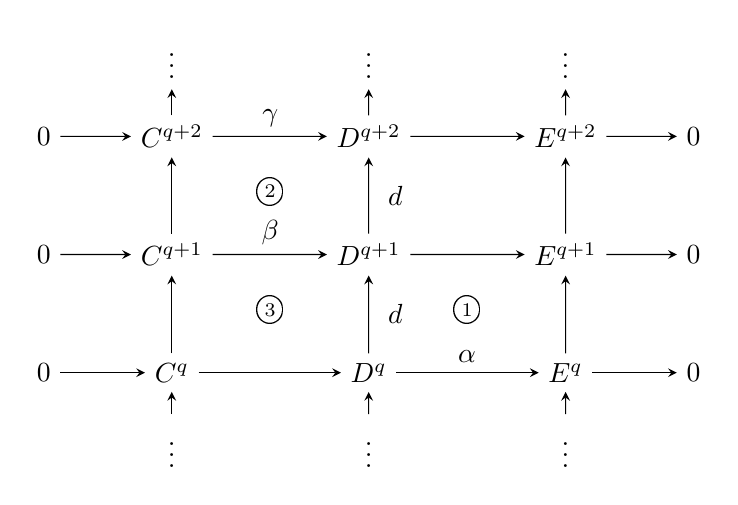
\begin{tikzpicture}[baseline={(current bounding box.center)},>=stealth,scale=1.25]
\node (zLq) at (-1.3,0) {$0$};   \node (Cq) at (0,0) {$C^{q}$};     \node (Dq) at (2,0) {$D^{q}$};     \node (Eq) at (4,0) {$E^{q}$};     \node (zRq) at (5.3,0) {$0$};
\node (zLu) at (-1.3,1.2) {$0$}; \node (Cu) at (0,1.2) {$C^{q+1}$}; \node (Du) at (2,1.2) {$D^{q+1}$}; \node (Eu) at (4,1.2) {$E^{q+1}$}; \node (zRu) at (5.3,1.2) {$0$};
\node (zLv) at (-1.3,2.4) {$0$}; \node (Cv) at (0,2.4) {$C^{q+2}$}; \node (Dv) at (2,2.4) {$D^{q+2}$}; \node (Ev) at (4,2.4) {$E^{q+2}$}; \node (zRv) at (5.3,2.4) {$0$};
\foreach \A/\B in {zLq/Cq,Cq/Dq,Dq/Eq,Eq/zRq,zLu/Cu,Cu/Du,Du/Eu,Eu/zRu,zLv/Cv,Cv/Dv,Dv/Ev,Ev/zRv}{\draw[->] (\A) -- (\B);}
\foreach \A/\B in {Cq/Cu,Cu/Cv,Dq/Du,Du/Dv,Eq/Eu,Eu/Ev}{\draw[->] (\A) -- (\B);}
\foreach \N in {Cq,Dq,Eq}{\node at (\N |- 0,-0.75) {$\vdots$}; \draw[->] (\N |- 0,-0.42) -- (\N);}
\foreach \N in {Cv,Dv,Ev}{\node at (\N |- 0,3.2) {$\vdots$}; \draw[->] (\N) -- (\N |- 0,2.88);}
\node[above] at (1,2.4) {$\gamma$};
\node[above] at (1,1.2) {$\beta$};
\node[above] at (3,0) {$\alpha$};
\node[right] at (2.1,0.6) {$d$};
\node[right] at (2.1,1.8) {$d$};
\node at (3,0.6) {\textcircled{\scriptsize 1}};
\node at (1,0.6) {\textcircled{\scriptsize 3}};
\node at (1,1.8) {\textcircled{\scriptsize 2}};
\end{tikzpicture}
\end{equation}

by the exactness of the horizontal sequences, $d(\tilde{\sigma})$ must be in the image of $\beta$. Thus there is an element $\sigma'\in C^{q+1}$ such that $\beta(\sigma')=d(\tilde{\sigma})$. It follows from the commutativity of the square $\textcircled{2}$, the injectivity of $\gamma$, and the fact that $d\circ d=0$ that $\sigma'$ is a cocycle. Now, $\sigma'$ is not uniquely determined by $\sigma$ because of the choice involved in the selection of $\tilde{\sigma}\in D^{q}$ such that $\alpha(\tilde{\sigma})=\sigma$. However, it is easily seen by a quick chase around the square $\textcircled{3}$ that $\sigma'$ is uniquely determined by $\sigma$ up to a coboundary. Thus we have a well-defined map

\begin{equation}
\label{eq:5.17:5}
Z^{q}(E^{*})\to H^{q+1}(C^{*}),
\end{equation}

which is easily seen to be a homomorphism. It is also readily seen that  $ B^{q}(E^{*}) $ is in the kernel of (5); hence (5) yields a homomorphism defined on the quotient  $ Z^{q}(E^{*})/B^{q}(E^{*}) $. This by definition is the desired homomorphism (1).

Checking the exactness of (2) involves checking exactness at  $ H^{q}(C^{*}) $, at  $ H^{q}(D^{*}) $, and at  $ H^{q}(E^{*}) $—and at each of these three stages we have to check two inclusion relations. These six steps in the proof of the exactness of (2) can be verified by simple chases around the diagram (4). We leave the details to the reader.

\[
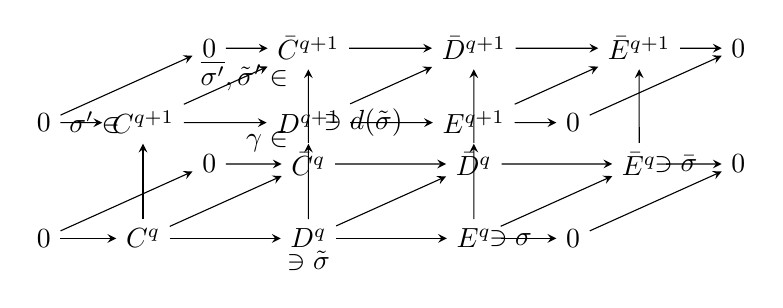
\begin{tikzpicture}[baseline={(current bounding box.center)},>=stealth,scale=1.05]
% front plane: unbarred complexes
\node (zLfq) at (-1.2,0) {$0$};   \node (Cfq) at (0,0) {$C^{q}$};     \node (Dfq) at (2,0) {$D^{q}$};     \node (Efq) at (4,0) {$E^{q}$};     \node (zRfq) at (5.2,0) {$0$};
\node (zLfu) at (-1.2,1.4) {$0$}; \node (Cfu) at (0,1.4) {$C^{q+1}$}; \node (Dfu) at (2,1.4) {$D^{q+1}$}; \node (Efu) at (4,1.4) {$E^{q+1}$}; \node (zRfu) at (5.2,1.4) {$0$};
% back plane: barred complexes
\node (zLbq) at (0.8,0.9) {$0$};  \node (Cbq) at (2,0.9) {$\bar{C}^{q}$};     \node (Dbq) at (4,0.9) {$\bar{D}^{q}$};     \node (Ebq) at (6,0.9) {$\bar{E}^{q}$};     \node (zRbq) at (7.2,0.9) {$0$};
\node (zLbu) at (0.8,2.3) {$0$};  \node (Cbu) at (2,2.3) {$\bar{C}^{q+1}$}; \node (Dbu) at (4,2.3) {$\bar{D}^{q+1}$}; \node (Ebu) at (6,2.3) {$\bar{E}^{q+1}$}; \node (zRbu) at (7.2,2.3) {$0$};
\foreach \A/\B in {zLfq/Cfq,Cfq/Dfq,Dfq/Efq,Efq/zRfq,zLfu/Cfu,Cfu/Dfu,Dfu/Efu,Efu/zRfu,zLbq/Cbq,Cbq/Dbq,Dbq/Ebq,Ebq/zRbq,zLbu/Cbu,Cbu/Dbu,Dbu/Ebu,Ebu/zRbu}{\draw[->] (\A) -- (\B);}
\foreach \A/\B in {Cfq/Cfu,Dfq/Dfu,Efq/Efu,Cbq/Cbu,Dbq/Dbu,Ebq/Ebu}{\draw[->] (\A) -- (\B);}
\foreach \A/\B in {zLfq/zLbq,Cfq/Cbq,Dfq/Dbq,Efq/Ebq,zRfq/zRbq,zLfu/zLbu,Cfu/Cbu,Dfu/Dbu,Efu/Ebu,zRfu/zRbu}{\draw[->] (\A) -- (\B);}
% element labels
\node[right=2pt] at (Efq) {$\ni\sigma$};
\node[below=1pt] at (Dfq) {$\ni\tilde{\sigma}$};
\node[right=2pt] at (Dfu) {$\ni d(\tilde{\sigma})$};
\node[left=2pt] at (Cfu) {$\sigma'\in{}$};
\node[below left=1pt] at (Cbu) {$\overline{\sigma'},\tilde{\sigma}'\in{}$};
\node[above left=1pt] at (Cbq) {$\gamma\in{}$};
\node[right=2pt] at (Ebq) {$\ni\bar{\sigma}$};
\end{tikzpicture}
\]

To prove (3), we have to follow some elements around the above commutative lattice.

We start with a cocycle $\sigma\in E^{q}$ and lift it back to $\tilde{\sigma}\in D^{q}$, which we map to $d(\tilde{\sigma})\in D^{q+1}$, which we have seen is the image of an element $\sigma'\in C^{q+1}$, which in turn we map to $\overline{\sigma'}\in\bar{C}^{q+1}$. Then $\overline{\sigma'}$ is a cocycle in $\bar{C}^{q+1}$ and is a representative of the cohomology class in $H^{q+1}(\bar{C}^{*})$ into which the cohomology class of $\sigma$ in $H^{q}(E^{*})$ is mapped under the composition $H^{q}(E^{*})\xrightarrow{\partial}H^{q+1}(C^{*})\to H^{q+1}(\bar{C}^{*})$. On the other hand, we can first map $\sigma$ to $\bar{\sigma}\in\bar{E}^{q}$, then lift back to $\tilde{\bar{\sigma}}\in\bar{D}^{q}$, map to $d(\tilde{\bar{\sigma}})\in\bar{D}^{q+1}$, and lift back to $\tilde{\sigma}'\in\bar{C}^{q+1}$. Then $\tilde{\sigma}'$ is a cocycle in $\bar{C}^{q+1}$ which represents the cohomology class in $H^{q+1}(\bar{C}^{*})$ into which the cohomology class of $\sigma$ is mapped under the composition $H^{q}(E^{*})\to H^{q}(\bar{E}^{*})\xrightarrow{\partial}H^{q+1}(\bar{C}^{*})$. To prove (3), we need only check that $\overline{\sigma'}-\tilde{\sigma}'$ is a coboundary. Now $\tilde{\sigma}\in D^{q}$ maps to an element $\bar{\tilde{\sigma}}\in\bar{D}^{q}$, and elements $\bar{\tilde{\sigma}}$ and $\tilde{\bar{\sigma}}$ of $\bar{D}^{q}$ both map to $\bar{\sigma}\in\bar{E}^{q}$; hence there is an element $\gamma\in\bar{C}^{q}$ which maps to $(\bar{\tilde{\sigma}}-\tilde{\bar{\sigma}})$. One can easily check that $d\gamma=\overline{\sigma'}-\tilde{\sigma}'$, which completes the proof of \hyperref[thm:5.17]{Proposition 5.17}.

After a few trials the reader should find that these proofs by “diagram chase” become quite routine, albeit tedious. In the future we shall leave all such proofs as exercises.

\end{proof}

\section{Axiomatic Sheaf Cohomology}


\begin{definition}\label{thm:5.18}
A sheaf cohomology theory $\mathcal{H}$ for $M$ with coefficients in sheaves of $K$-modules over $M$ consists of \index{Sheaf cohomology theory}

(I) a $K$-module $H^q(M,\mathcal{S})$ for each sheaf $\mathcal{S}$ and for each integer $q$,

(II) a homomorphism  $ H^q(M,\mathcal{S}) \to H^q(M,\mathcal{S}') $ for each homomorphism  $ \mathcal{S} \to \mathcal{S}' $ and for each integer  $ q $, and

(III) a homomorphism $H^{q}(M,\mathcal{S}^{\prime \prime}) \to H^{q+1}(M,\mathcal{S}^{\prime})$ for each short exact sequence $0 \to \mathcal{S}^{\prime} \to \mathcal{S} \to \mathcal{S}^{\prime \prime} \to 0$ and for each integer $q$,

such that the properties (a)–(f) hold:

(a) $H^{q}(M,\mathcal{S}) = 0$ for $q < 0$, and there is an isomorphism $H^{0}(M,\mathcal{S}) \cong \Gamma(\mathcal{S})$ such that for each homomorphism $\mathcal{S} \to \mathcal{S}'$ the diagram

\[
\begin{array}{c}H^{0}(M,\mathcal{S})\cong\Gamma(\mathcal{S})\\\downarrow\quad\downarrow\\H^{0}(M,\mathcal{S}^{\prime})\cong\Gamma(\mathcal{S}^{\prime})\end{array}
\]

commutes.

(b)  $ H^{q}(M,\mathcal{S}) =0$ for all $q>0$ if  $ \mathcal{S} $ is a fine sheaf.

(c) If $0 \to \mathcal{S}' \to \mathcal{S} \to \mathcal{S}'' \to 0$ is exact, then the following is exact:

\[
\cdots\to H^{q}(M,\mathcal{S}^{\prime})\to H^{q}(M,\mathcal{S})\to H^{q}(M,\mathcal{S}^{\prime \prime})\to H^{q+1}(M,\mathcal{S}^{\prime})\to\cdots.
\]

(d) The identity homomorphism id: $\mathcal{S} \to \mathcal{S}$ induces the identity homomorphism id: $H^{q}(M,\mathcal{S}) \to H^{q}(M,\mathcal{S})$.

(e) If the diagram

\[
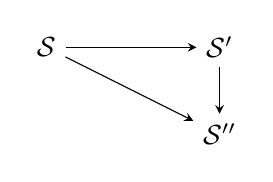
\begin{tikzpicture}[baseline={(current bounding box.center)},>=stealth]
\node (S) at (0,1.1) {$\mathcal{S}$};
\node (S1) at (2.2,1.1) {$\mathcal{S}'$};
\node (S2) at (2.2,0) {$\mathcal{S}''$};
\draw[->] (S) -- (S1);
\draw[->] (S1) -- (S2);
\draw[->] (S) -- (S2);
\end{tikzpicture}
\]

commutes, then for each $q$ so does the diagram

\[
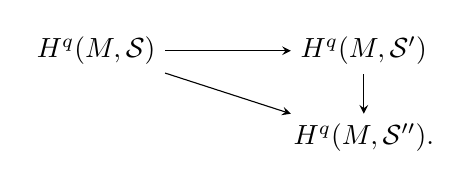
\begin{tikzpicture}[baseline={(current bounding box.center)},>=stealth]
\node (S) at (0,1.1) {$H^{q}(M,\mathcal{S})$};
\node (S1) at (3.4,1.1) {$H^{q}(M,\mathcal{S}')$};
\node (S2) at (3.4,0) {$H^{q}(M,\mathcal{S}'').$};
\draw[->] (S) -- (S1);
\draw[->] (S1) -- (S2);
\draw[->] (S) -- (S2);
\end{tikzpicture}
\]

(f) For each homomorphism of short exact sequences of sheaves

\[
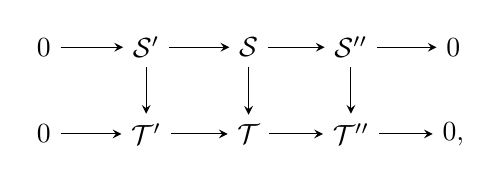
\begin{tikzpicture}[baseline={(current bounding box.center)},>=stealth]
\node (z1) at (0,1.1) {$0$}; \node (S1) at (1.3,1.1) {$\mathcal{S}'$}; \node (S) at (2.6,1.1) {$\mathcal{S}$}; \node (S2) at (3.9,1.1) {$\mathcal{S}''$}; \node (z2) at (5.2,1.1) {$0$};
\node (w1) at (0,0) {$0$}; \node (T1) at (1.3,0) {$\mathcal{T}'$}; \node (T) at (2.6,0) {$\mathcal{T}$}; \node (T2) at (3.9,0) {$\mathcal{T}''$}; \node (w2) at (5.2,0) {$0,$};
\foreach \A/\B in {z1/S1,S1/S,S/S2,S2/z2,w1/T1,T1/T,T/T2,T2/w2,S1/T1,S/T,S2/T2}{\draw[->] (\A) -- (\B);}
\end{tikzpicture}
\]

the following diagram commutes:

\[
\begin{matrix}{H^{q}(M,\mathcal{S}^{\prime\prime})\to H^{q+1}(M,\mathcal{S}^{\prime})}\\ {\downarrow\quad\downarrow}\\ {H^{q}(M,\mathcal{T}^{\prime\prime})\to H^{q+1}(M,\mathcal{T}^{\prime}).}\\ \end{matrix}
\]

The module $H^{q}(M,\mathcal{S})$ is called the $q$th cohomology module of $M$ with coefficients in the sheaf $\mathcal{S}$ relative to the cohomology theory $\mathcal{H}$.

\end{definition}

\begin{definition}\label{thm:5.19}
An exact sheaf sequence

\begin{equation}
\label{eq:5.19:1}
0\to\mathcal{A}\to\mathcal{C}_{0}\to\mathcal{C}_{1}\to\mathcal{C}_{2}\to\cdots
\end{equation}

is called a resolution of the sheaf $\mathcal{A}$. The resolution (1) is called fine (respectively torsionless) if each of the sheaves $\mathcal{C}_{i}$ is fine (respectively torsionless). \index{Resolution}

With each resolution (1) of $\mathcal{A}$ and each sheaf $\mathcal{S}$ we associate a cochain complex

\begin{equation}
\label{eq:5.19:2}
\cdots\to0\to\Gamma(\mathcal{C}_{0}\otimes\mathcal{S})\to\Gamma(\mathcal{C}_{1}\otimes\mathcal{S})\to\Gamma(\mathcal{C}_{2}\otimes\mathcal{S})\to\cdots
\end{equation}

which we shall denote by $\Gamma(\mathcal{C}^*\otimes\mathcal{S})$. For $q\geq0$ the module of $q$-cochains is $\Gamma(\mathcal{C}_q\otimes\mathcal{S})$, whereas for $q<0$ the module of $q$-cochains is the zero module. Note carefully that this cochain complex does not contain the module $\Gamma(\mathcal{A}\otimes\mathcal{S})$. The homomorphisms in (2) are those induced by the homomorphisms $\mathcal{C}_i\otimes\mathcal{S}\to\mathcal{C}_{i+1}\otimes\mathcal{S}$ which are the tensor product of the homomorphisms of (1) with id: $\mathcal{S}\to\mathcal{S}$. The exactness of (1) implies that in

\begin{equation}
\label{eq:5.19:3}
\cdots\to0\to\mathcal{C}_{0}\otimes\mathcal{S}\to\mathcal{C}_{1}\otimes\mathcal{S}\to\mathcal{C}_{2}\otimes\mathcal{S}\to\cdots
\end{equation}

the image of each homomorphism is contained in the kernel of the next, and this in turn implies that (2) is indeed a cochain complex.

A homomorphism $\mathcal{S} \to \mathcal{S}'$ when tensored with the identity homomorphisms of the sheaves $\mathcal{C}_i$ yields homomorphisms $\mathcal{C}_i \otimes \mathcal{S} \to \mathcal{C}_i \otimes \mathcal{S}'$. These, in turn, induce homomorphisms $\Gamma(\mathcal{C}_i \otimes \mathcal{S}) \to \Gamma(\mathcal{C}_i \otimes \mathcal{S}')$, which commute with the coboundary homomorphisms of the respective cochain complexes and thus determine a cochain map

\begin{equation}
\label{eq:5.19:4}
\Gamma(\mathcal{C}^{*}\otimes\mathcal{S})\to\Gamma(\mathcal{C}^{*}\otimes\mathcal{S}^{\prime}).
\end{equation}

\end{definition}

\subsection{Existence of Cohomology Theories}\label{thm:5.20} We shall now show that each fine torsionless resolution of the constant sheaf  $ \mathcal{K} = M \times K $,

\begin{equation}
\label{eq:5.20:1}
0\to\mathcal{K}\to\mathcal{C}_{0}\to\mathcal{C}_{1}\to\mathcal{C}_{2}\to\cdots,
\end{equation}

canonically determines a cohomology theory for $M$ with coefficients in sheaves of $K$-modules over $M$. The existence of such resolutions will be amply demonstrated in the later sections in which the classical cohomology theories are discussed. In particular, see \eqref{eq:5.26:7} and \eqref{eq:5.26:11}. We therefore assume that we are given a fine torsionless resolution (1). Then we obtain a cohomology theory as follows: \index{Torsionless resolution}

(I) With a sheaf $\mathcal{S}$ and each integer $q$ we associate the $q$th cohomology module of the cochain complex  $ \Gamma(\mathcal{C}^* \otimes \mathcal{S}) $; that is, we set

\[
H^{q}(M,\mathcal{S})=H^{q}\big(\Gamma(\mathcal{C}^{\ast}\otimes\mathcal{S})\big).
\]

(II) With each homomorphism $\mathcal{S}\to\mathcal{S}^{\prime}$ and each integer $q$ we associate the homomorphism $H^{q}(M,\mathcal{S})\to H^{q}(M,\mathcal{S}^{\prime})$ induced, according to \eqref{eq:5.16:4}, by the cochain map $\Gamma(\mathcal{C}^{*}\otimes\mathcal{S})\to\Gamma(\mathcal{C}^{*}\otimes\mathcal{S}^{\prime})$ of \eqref{eq:5.19:4}.

(III) Each short exact sheaf sequence

\[
0\to\mathcal{S}^{\prime}\to\mathcal{S}\to\mathcal{S}^{\prime \prime}\to0
\]

induces, in view of \hyperref[thm:5.15]{Theorem 5.15} and the fact that the $\mathcal{C}_{i}$ are fine torsionless sheaves, a short exact sequence of cochain maps

\[
0\to\Gamma(\mathcal{C}^{*}\otimes\mathcal{S}^{\prime})\to\Gamma(\mathcal{C}^{*}\otimes\mathcal{S})\to\Gamma(\mathcal{C}^{*}\otimes\mathcal{S}^{\prime\prime})\to0
\]

with which, according to \eqref{eq:5.17:1}, there is associated a homomorphism  $ H^{q}(\Gamma(\mathcal{C}^*\otimes\mathcal{S}''))\to H^{q+1}(\Gamma(\mathcal{C}^*\otimes\mathcal{S}')) $. This, by definition, is the homomorphism $H^{q}(M,\mathcal{S}'') \to H^{q+1}(M,\mathcal{S}')$ that we associate with the short exact sequence $0 \to \mathcal{S}' \to \mathcal{S} \to \mathcal{S}'' \to 0$ and the integer  $ q $.

The fact that axiom \hyperref[thm:5.18]{5.18(d)} for a cohomology theory is satisfied is immediately apparent. The remark immediately following \eqref{eq:5.16:4} implies that axiom (e) is satisfied. Axioms (c) and (f) are consequences of 5.17.

Now let $\mathcal{Z}_{q}$ be the kernel of $\mathcal{C}_{q}\to\mathcal{C}_{q+1}$. Then it follows from the exactness of (1) that

\begin{equation}
\label{eq:5.20:2}
0\to\mathcal{Z}_{q}\to\mathcal{C}_{q}\to\mathcal{Z}_{q+1}\to0
\end{equation}

is exact; and since $\mathcal{Z}_{q}$ is a subsheaf of the torsionless sheaf $\mathcal{C}_{q}$, then $\mathcal{Z}_{q}$ is also torsionless. It follows from \hyperref[thm:5.15]{Theorem 5.15} that for any sheaf $S$ the sequence

\begin{equation}
\label{eq:5.20:3}
0\to\mathcal{Z}_{q}\otimes\mathcal{S}\to\mathcal{C}_{q}\otimes\mathcal{S}\to\mathcal{Z}_{q+1}\otimes\mathcal{S}\to0
\end{equation}

is exact; and from (3) and \eqref{eq:5.11:2} we obtain the exact sequence

\begin{equation}
\label{eq:5.20:4}
0\to\Gamma(\mathcal{Z}_{q}\otimes\mathcal{S})\to\Gamma(\mathcal{C}_{q}\otimes\mathcal{S})\to\Gamma(\mathcal{Z}_{q+1}\otimes\mathcal{S}).
\end{equation}

In particular,  $ \Gamma(\mathcal{Z}_q \otimes \mathcal{S}) \to \Gamma(\mathcal{C}_q \otimes \mathcal{S}) $ is an injection, so since the homomorphism

\begin{equation}
\label{eq:5.20:5}
\Gamma(\mathcal{C}_{q}\otimes\mathcal{S})\to\Gamma(\mathcal{C}_{q+1}\otimes\mathcal{S})
\end{equation}

is the composition

\begin{equation}
\label{eq:5.20:6}
\Gamma(\mathcal{C}_{q}\otimes\mathcal{S})\to\Gamma(\mathcal{Z}_{q+1}\otimes\mathcal{S})\to\Gamma(\mathcal{C}_{q+1}\otimes\mathcal{S}),
\end{equation}

it follows from (4) that the kernel of (5) is simply the submodule $\Gamma(\mathcal{Z}_q \otimes \mathcal{S})$ of $\Gamma(\mathcal{C}_q \otimes \mathcal{S})$. Thus for  $ q \geq 0 $,

\begin{equation}
\label{eq:5.20:7}
H^{q}(M,\mathcal{S})=H^{q}\big(\Gamma(\mathcal{C}^{*}\otimes\mathcal{S})\big)=\Gamma(\mathcal{Z}_{q}\otimes\mathcal{S})/\operatorname{Im}\big(\Gamma(\mathcal{C}_{q-1}\otimes\mathcal{S})\big).
\end{equation}

Now, if $\mathcal{S}$ happens to be a fine sheaf, then according to \hyperref[thm:5.15]{Theorem 5.15} the full sequence

\begin{equation}
\label{eq:5.20:8}
0\to\Gamma(\mathcal{Z}_{q-1}\otimes\mathcal{S})\to\Gamma(\mathcal{C}_{q-1}\otimes\mathcal{S})\to\Gamma(\mathcal{Z}_{q}\otimes\mathcal{S})\to0
\end{equation}

is exact; and (8) together with (7) implies that

\[
H^{q}(M,\mathcal{S})=0\quad\mathrm{for}\;q>0.
\]

Thus axiom (b) is satisfied.

Finally, it is evident that $H^{q}(M,\mathcal{S}) = 0$ for $q < 0$, and for $q = 0$ the isomorphism

\begin{equation}
\label{eq:5.20:9}
\mathcal{K}\to\mathcal{Z}_{0}\subset\mathcal{C}_{0}
\end{equation}

induces, for an arbitrary sheaf $\mathcal{S}$, an isomorphism

\begin{equation}
\label{eq:5.20:10}
\mathcal{S}\cong\mathcal{K}\otimes\mathcal{S}\xrightarrow{\cong}\mathcal{Z}_{0}\otimes\mathcal{S}
\end{equation}

and thus an isomorphism

\[
\Gamma(\mathcal{S})\xrightarrow{\simeq}\Gamma(\mathcal{Z}_{0}\otimes\mathcal{S})=H^{0}(M,\mathcal{S}),
\]

which clearly satisfies

\[
\begin{array}{c}\Gamma(\mathcal{S})\cong H^{0}(M,\mathcal{S})\\\downarrow\quad\downarrow\\\Gamma(\mathcal{S}^{\prime})\cong H^{0}(M,\mathcal{S}^{\prime})\end{array}
\]

for each homomorphism  $ \mathcal{S} \to \mathcal{S}' $. Thus axiom (a) is satisfied.

\begin{definition}\label{thm:5.21}
Let $\mathcal{H}$ and $\tilde{\mathcal{H}}$ be two sheaf cohomology theories on $M$ with coefficients in sheaves of $K$-modules over $M$. A homomorphism of the cohomology theory $\mathcal{H}$ to the theory $\tilde{\mathcal{H}}$ consists of a homomorphism

\begin{equation}
\label{eq:5.21:1}
H^{q}(M,\mathcal{S})\to\tilde{H}^{q}(M,\mathcal{S})
\end{equation}

for each sheaf $\mathcal{S}$ and for each integer $q$, such that the following conditions hold:

(a) For q = 0, the diagram

\[
\begin{array}{c}H^{0}(M,\mathcal{S})\cong\Gamma(\mathcal{S})\\\downarrow\quad\downarrow\\\tilde{H}^{0}(M,\mathcal{S})\cong\Gamma(\mathcal{S})\end{array}
\]

commutes.

(b) For each homomorphism  $ \mathcal{S} \to \mathcal{T} $ and each integer  $ q $ the diagram

\[
\begin{matrix}{H^{q}(M,\mathcal{S})\to H^{q}(M,\mathcal{T})}\\ {\downarrow\quad\downarrow}\\ {\tilde{H}^{q}(M,\mathcal{S})\to\tilde{H}^{q}(M,\mathcal{T})}\\ \end{matrix}
\]

commutes.

(c) For each short exact sequence of sheaves

\[
0\to\mathcal{R}\to\mathcal{S}\to\mathcal{T}\to0
\]

the following diagram commutes for each integer $q$:

\[
\begin{array}{c}H^{q}(M,\mathcal{T})\xrightarrow{\partial}H^{a+1}(M,\mathcal{R})\\\downarrow\quad\downarrow\\\tilde{H}^{q}(M,\mathcal{T})\xrightarrow{\partial}\tilde{H}^{a+1}(M,\mathcal{R}).\end{array}
\]

An isomorphism $\mathcal{H}\to\tilde{\mathcal{H}}$ is a homomorphism in which each of the homomorphisms $H^{q}(M,\mathcal{S})\to\tilde{H}^{q}(M,\mathcal{S})$ are isomorphisms. The identity homomorphism of $\mathcal{H}$ with itself is the homomorphism $\mathcal{H}\to\mathcal{H}$ which assigns the identity homomorphism $H^{q}(M,\mathcal{S})\to H^{q}(M,\mathcal{S})$ to each sheaf $\mathcal{S}$ and each integer $q$.

\end{definition}

We are now going to prove that there is a unique homomorphism between any two sheaf cohomology theories on $M$. However, first we need to introduce the notion of the sheaf of germs of discontinuous sections of a sheaf $S$.

\subsection{The Sheaf of Germs of Discontinuous Sections of $\mathcal{S}$}\label{thm:5.22} Let $\mathcal{S}$ be a sheaf on $M$. By a discontinuous section of $\mathcal{S}$ over the open set $U \subset M$ we mean any map $f: U \to \mathcal{S}$, continuous or not, such that $\pi \circ f = \mathrm{id}$. The assignment to each open set $U \subset M$ of the module of all discontinuous sections of $\mathcal{S}$ over $U$ yields a presheaf whose associated sheaf $\mathcal{S}_0$ is called the sheaf of germs of discontinuous sections of $\mathcal{S}$.

The important property of $\mathcal{S}_{0}$ that we shall need is that $\mathcal{S}_{0}$ is always a fine sheaf. For let $\{U_{i}\}$ be a locally finite open cover of $M$. Choose a refinement $\{V_{i}\}$ such that $\overline{V}_{i} \subset U_{i}$ for each $i$ (Exercise 3, Chapter 1). (For such a refinement on a general paracompact Hausdorff space, see [13, Ch. 5, Problem V(a)].) Associate with each point of $M$ a set $V_{i}$ containing it, and then for each $i$ define a function $\varphi_{i}$ on $M$ to have the value 1 at all points associated with $V_{i}$ and to have the value 0 elsewhere. It follows that $\operatorname{supp} \varphi_{i} \subset U_{i}$ and $\sum \varphi_{i} \equiv 1$. We associate with $\varphi_{i}$ an endomorphism $\widetilde{I}_{i}$ of the presheaf of discontinuous sections of 8 by defining

\begin{equation}
\label{eq:5.22:1}
\tilde{l}_{i}(s)(m)=\varphi_{i}(m)s(m)
\end{equation}

for each discontinuous section $s$ of $\mathcal{S}$ over an open set $U \subset M$ and each $m \in U$. The presheaf endomorphisms $\tilde{l}_{i}$ induce endomorphisms $l_{i}$ of the sheaf $\mathcal{S}_{0}$ of germs of discontinuous sections of $\mathcal{S}$. It is immediate that the $\{l_{i}\}$ form a partition of unity of $\mathcal{S}_{0}$ subordinate to the locally finite cover $\{U_{i}\}$ of $M$. Thus $\mathcal{S}_{0}$ is a fine sheaf, as claimed.

There is a natural injection of $\mathcal{S}$ into $\mathcal{S}_0$; namely, each element of the stalk $\mathcal{S}_m$ is the value at $m$ of a (continuous) section $s$ of $\mathcal{S}$ defined on some neighborhood of $m$, and we map $s(m)$ to the germ of $s$ at $m$ in $\mathcal{S}_0$. If we let $\overline{\mathcal{S}}$ denote the quotient sheaf $\mathcal{S}_0/\mathcal{S}$, then for each sheaf $\mathcal{S}$ we have constructed a short exact sequence

\begin{equation}
\label{eq:5.22:2}
0\to\mathcal{S}\to\mathcal{S}_{0}\to\overline{{\mathcal{S}}}\to0
\end{equation}

in which the middle sheaf is fine.

\begin{theorem}\label{thm:5.23}
Let $\mathcal{H}$ and $\tilde{\mathcal{H}}$ be cohomology theories on $M$ with coefficients in sheaves of $K$-modules over $M$. Then there exists a unique homomorphism of $\mathcal{H}$ to $\tilde{\mathcal{H}}$.

\end{theorem}

\begin{proof}
We first prove uniqueness. Suppose that we have a homomorphism of $\mathcal{H}$ to $\tilde{\mathcal{H}}$, and let a sheaf $\mathcal{S}$ be given. Then it follows from the axioms 5.18 and 5.21 applied to the exact sequence \eqref{eq:5.22:2}, in which, you recall, the sheaf $\mathcal{S}_{0}$ is fine, that we have a commutative diagram

\begin{equation}
\label{eq:5.23:1}
\begin{array}{c}\Gamma(\mathcal{S}_{0})\rightarrow\Gamma(\overline{\mathcal{S}})\rightarrow H^{1}(M,\mathcal{S})\rightarrow0\\\downarrow\mathrm{id}\quad\downarrow\mathrm{id}\quad\downarrow\\\Gamma(\mathcal{S}_{0})\rightarrow\Gamma(\overline{\mathcal{S}})\rightarrow\tilde{H}^{1}(M,\mathcal{S})\rightarrow0;\end{array}
\end{equation}

and for each $q \geq 2$ we have a commutative diagram

\begin{equation}
\label{eq:5.23:2}
\begin{array}{c}0\to H^{q-1}(M,\overline{\mathcal{S}})\to H^{q}(M,\mathcal{S})\to0\\\downarrow\quad\downarrow\\0\to\check{H}^{q-1}(M,\overline{\mathcal{S}})\to\check{H}^{q}(M,\mathcal{S})\to0.\end{array}
\end{equation}

Note that in both (1) and (2) the rows are exact. Now uniqueness of the homomorphisms \eqref{eq:5.21:1} follows for $q=0$ from \hyperref[thm:5.21]{5.21(a)}, follows for $q=1$ from (1), and follows inductively for $q>1$ from (2).

We now show the existence of a homomorphism of the theory $\mathcal{H}$ to the theory $\widetilde{\mathcal{H}}$. We define the homomorphisms for $q=0$ by $5.21(a)$, and it follows immediately that $5.21(b)$ is satisfied for the case $q=0$. We define the homomorphisms $\eqref{eq:5.21:1}$ for $q=1$ by (1), and inductively for $q>1$ by (2). To prove that this indeed defines a homomorphism of $\mathcal{H}$ to $\widetilde{\mathcal{H}}$, it remains to show that $5.21(b)$ holds for $q>0$ and that $5.21(c)$ holds for all $q$.

Now, \hyperref[thm:5.21]{5.21(b)} follows for $q = 1$ from the following lattice constructed from two copies of (1):

\begin{center}
\begin{tikzpicture}[>=stealth,every node/.style={font=\small}]
% front face: theory H, sheaf S ; back face: sheaf T ; lower copies: theory H~
\node (A1) at (0,0) {$\Gamma(\bar{\mathcal{S}})$};
\node (B1) at (3.4,0) {$H^{1}(M,\mathcal{S})$};
\node (C1) at (6.2,0) {$0$};
\node (A2) at (0,-2.2) {$\Gamma(\bar{\mathcal{S}})$};
\node (B2) at (3.4,-2.2) {$\widetilde{H}^{1}(M,\mathcal{S})$};
\node (C2) at (6.2,-2.2) {$0$};
\node (A1b) at (1.6,-1.0) {$\Gamma(\bar{\mathcal{T}})$};
\node (B1b) at (5.0,-1.0) {$H^{1}(M,\mathcal{T})$};
\node (C1b) at (7.8,-1.0) {$0$};
\node (A2b) at (1.6,-3.2) {$\Gamma(\bar{\mathcal{T}})$};
\node (B2b) at (5.0,-3.2) {$\widetilde{H}^{1}(M,\mathcal{T})$};
\node (C2b) at (7.8,-3.2) {$0$};
\draw[->] (A1) -- (B1); \draw[->] (B1) -- (C1);
\draw[->] (A2) -- (B2); \draw[->] (B2) -- (C2);
\draw[->] (A1b) -- (B1b); \draw[->] (B1b) -- (C1b);
\draw[->] (A2b) -- (B2b); \draw[->] (B2b) -- (C2b);
\draw[->] (A1) -- (A1b); \draw[->] (B1) -- (B1b); \draw[->] (C1) -- (C1b);
\draw[->] (A2) -- (A2b); \draw[->] (B2) -- (B2b); \draw[->] (C2) -- (C2b);
\draw[->] (A1) -- (A2); \draw[->] (B1) -- (B2); \draw[->] (C1) -- (C2);
\draw[->] (A1b) -- (A2b); \draw[->] (B1b) -- (B2b); \draw[->] (C1b) -- (C2b);
\node at (5.55,-2.35) {\text{①}};
\end{tikzpicture}
\end{center}

In the lattice, the commutativity of the right-hand face ① is forced by the a priori commutativity of all the other faces, and \hyperref[thm:5.21]{5.21(b)} follows inductively for $q>1$ from the analogous lattice constructed from (2).

As for \hyperref[thm:5.21]{5.21(c)}, suppose that a short exact sequence

\begin{equation}
\label{eq:5.23:4}
0\to\mathcal{R}\to\mathcal{S}\to\mathcal{T}\to0
\end{equation}

is given. Let $\mathcal{R}_{0}$ and $\mathcal{S}_{0}$ be the sheaves of germs of discontinuous sections of $\mathcal{R}$ and $\mathcal{S}$ respectively. The composition $\mathcal{R}\to\mathcal{S}\to\mathcal{S}_{0}$ is an injection of $\mathcal{R}$ into $\mathcal{S}_{0}$; let $\mathcal{G}$ be the quotient sheaf $\mathcal{S}_{0}/\mathcal{R}$. As in 5.22, let $\overline{\mathcal{R}}=\mathcal{R}_{0}/\mathcal{R}$. Then there are uniquely determined homomorphisms $\mathcal{T}\to\mathcal{G}$ and $\overline{\mathcal{R}}\to\mathcal{G}$ such that the following diagram, in which the rows are exact, commutes:

\begin{equation}
\label{eq:5.23:5}
\begin{array}{c}0\longrightarrow\mathcal{R}\longrightarrow\mathcal{S}\longrightarrow\mathcal{T}\longrightarrow0\\\big\downarrow\mathrm{id}\quad\big\downarrow\quad\big\downarrow\\0\longrightarrow\mathcal{R}\longrightarrow\mathcal{S}_{0}\longrightarrow\mathcal{G}\longrightarrow0\\\big\uparrow\mathrm{id}\quad\big\uparrow\quad\big\uparrow\\0\longrightarrow\mathcal{R}\longrightarrow\mathcal{R}_{0}\longrightarrow\bar{\mathcal{R}}\longrightarrow0.\end{array}
\end{equation}

It follows from the cohomology axioms 5.18 applied to (5) that there are commutative diagrams

\begin{equation}
\label{eq:5.23:6}
\begin{array}{c}\cdots\longrightarrow\Gamma(\mathcal{S})\longrightarrow\Gamma(\mathcal{T})\longrightarrow H^{1}(M,\mathcal{R})\longrightarrow\cdots\\\big\downarrow\quad\big\downarrow\quad\big\downarrow\mathrm{id}\\\cdots\longrightarrow\Gamma(\mathcal{S}_{0})\longrightarrow\Gamma(\mathcal{G})\longrightarrow H^{1}(M,\mathcal{R})\longrightarrow0\\\big\uparrow\quad\big\uparrow\quad\big\uparrow\mathrm{id}\\\cdots\longrightarrow\Gamma(\mathcal{R}_{0})\longrightarrow\Gamma(\bar{\mathcal{R}})\longrightarrow H^{1}(M,\mathcal{R})\longrightarrow0\end{array}
\end{equation}

and (for  $ q \geq 1 $)

\begin{equation}
\label{eq:5.23:7}
\begin{array}{c}\cdots\longrightarrow H^{q}(M,\mathcal{S})\longrightarrow H^{q}(M,\mathcal{T})\longrightarrow H^{q+1}(M,\mathcal{R})\longrightarrow\cdots\\\big\downarrow\quad\big\downarrow\quad\big\downarrow\mathrm{id}\\0\longrightarrow H^{q}(M,\mathcal{G})\xrightarrow{\cong}H^{q+1}(M,\mathcal{R})\longrightarrow0\\\big\uparrow\quad\big\uparrow{\cong}\quad\big\uparrow\mathrm{id}\\0\longrightarrow H^{q}(M,\bar{\mathcal{R}})\xrightarrow{\cong}H^{q+1}(M,\mathcal{R})\longrightarrow0.\end{array}
\end{equation}

It follows from (6) that the homomorphism  $ H^{0}(M,\mathcal{T}) \to H^{1}(M,\mathcal{R}) $ is the composition

\begin{equation}
\label{eq:5.23:8}
H^0(M,\mathcal{T}) \xrightarrow{\cong} \Gamma(\mathcal{T}) \to \Gamma(\mathcal{G})/\operatorname{Im}\Gamma(\mathcal{S}_0) \xleftarrow{\cong} \Gamma(\overline{\mathcal{R}})/\operatorname{Im}\Gamma(\mathcal{R}_0) \xrightarrow{\cong} H^1(M,\mathcal{R})
\end{equation}

and it follows from (7) that the homomorphism  $ H^q(M,\mathcal{T}) \to H^{q+1}(M,\mathcal{R}) $ for  $ q \geq 1 $ is the composition

\begin{equation}
\label{eq:5.23:9}
H^{q}(M,\mathcal{T})\to H^{q}(M,\mathcal{G})\xleftarrow{\cong}H^{q}(M,\bar{\mathcal{R}})\xrightarrow{\cong}H^{q+1}(M,\mathcal{R}).
\end{equation}

From (8) and the corresponding sequence for the $\tilde{\mathcal{H}}$ theory we obtain the diagram

\begin{equation}
\label{eq:5.23:10}
\begin{array}{c c}{H^{0}(M,\mathcal{T})\xrightarrow{\cong}\Gamma(\mathcal{T})\to\Gamma(\mathcal{G})/\operatorname{Im}\Gamma(\mathcal{S}_{0})\xleftarrow{\cong}\Gamma(\bar{\mathcal{R}})/\operatorname{Im}\Gamma(\mathcal{R}_{0})\xrightarrow{\cong}H^{1}(M,\mathcal{R})}\\ {(10)\Big\downarrow\Big\downarrow\big\downarrow\operatorname{id}\Big\downarrow\big\downarrow\operatorname{id}\Big\downarrow\big\downarrow\operatorname{id}\Big\downarrow\big\downarrow}\\ {\tilde{H}^{0}(M,\mathcal{T})\xrightarrow{\cong}\Gamma(\mathcal{T})\to\Gamma(\mathcal{G})/\operatorname{Im}\Gamma(\mathcal{S}_{0})\xleftarrow{\cong}\Gamma(\bar{\mathcal{R}})/\operatorname{Im}\Gamma(\mathcal{R}_{0})\xrightarrow{\cong}\tilde{H}^{1}(M,\mathcal{R})}\\ \end{array}
\end{equation}

in which the first and last squares commute by the definitions of the homomorphisms $H^{0}(M,\mathcal{T})\to\tilde{H}^{0}(M,\mathcal{T})$ and $H^{1}(M,\mathcal{R})\to\tilde{H}^{1}(M,\mathcal{R})$, and the middle two squares trivially commute. Thus \hyperref[thm:5.21]{5.21(c)} is proved for $q=0$. From (9) and the corresponding sequence for the $\tilde{\mathcal{H}}$ theory we obtain the diagram

\begin{equation}
\label{eq:5.23:11}
\begin{array}{c}\boldsymbol{H}^{q}(\boldsymbol{M},\mathcal{T})\rightarrow\boldsymbol{H}^{q}(\boldsymbol{M},\mathcal{G})\xleftarrow{\cong}\boldsymbol{H}^{q}(\boldsymbol{M},\widetilde{\mathcal{R}})\xrightarrow{\cong}\boldsymbol{H}^{q+1}(\boldsymbol{M},\mathcal{R})\\\downarrow\quad\downarrow\quad\downarrow\quad\downarrow\quad\downarrow\\\widetilde{\boldsymbol{H}}^{q}(\boldsymbol{M},\mathcal{T})\rightarrow\widetilde{\boldsymbol{H}}^{q}(\boldsymbol{M},\mathcal{G})\xleftarrow{\cong}\widetilde{\boldsymbol{H}}^{q}(\boldsymbol{M},\widetilde{\mathcal{R}})\xrightarrow{\cong}\widetilde{\boldsymbol{H}}^{q+1}(\boldsymbol{M},\mathcal{R})\end{array}
\end{equation}

in which the last square commutes by definition of the homomorphism  $ H^{q+1}(M,\mathcal{R}) \to \tilde{H}^{q+1}(M,\mathcal{R}) $, and the first two squares commute by \hyperref[thm:5.21]{5.21(b)}. Thus \hyperref[thm:5.21]{5.21(c)} follows for  $ q \geq 1 $, and the proof of \hyperref[thm:5.23]{Theorem 5.23} is complete.

\end{proof}

\begin{corollary*}
A homomorphism of the cohomology theory $\mathcal{H}$ to the theory $\tilde{\mathcal{H}}$ must necessarily be an isomorphism. Consequently, any two cohomology theories on $M$ with coefficients in sheaves of $K$-modules over $M$ are uniquely isomorphic.

\end{corollary*}

\begin{proof}
Assume that a homomorphism $\mathcal{H}\to\tilde{\mathcal{H}}$ is given. By \hyperref[thm:5.23]{Theorem 5.23} there must also exist a homomorphism $\tilde{\mathcal{H}}\to\mathcal{H}$. The composition $\mathcal{H}\to\tilde{\mathcal{H}}\to\mathcal{H}$ must necessarily, by uniqueness, be the identity homomorphism of $\mathcal{H}$, and similarly the composition $\tilde{\mathcal{H}}\to\mathcal{H}\to\tilde{\mathcal{H}}$ must be the identity homomorphism of $\tilde{\mathcal{H}}$. It follows that the homomorphisms $\mathcal{H}\to\tilde{\mathcal{H}}$ and $\tilde{\mathcal{H}}\to\mathcal{H}$ are both isomorphisms.

\end{proof}

\subsection{\quad}\label{thm:5.24} Assume that

\begin{equation}
\label{eq:5.24:1}
\begin{array}{c}0\to\mathcal{K}\to\mathcal{C}_{0}\to\mathcal{C}_{1}\to\mathcal{C}_{2}\to\cdots\\ \downarrow\mathrm{id}\quad\downarrow\quad\downarrow\quad\downarrow\quad\downarrow\\ 0\to\mathcal{K}\to\widetilde{\mathcal{C}}_{0}\to\widetilde{\mathcal{C}}_{1}\to\widetilde{\mathcal{C}}_{2}\to\cdots\end{array}
\end{equation}

is a commutative diagram in which the rows are fine torsionless resolutions of the constant sheaf $\mathcal{K}$. We have seen in 5.20 that each of these resolutions determines a cohomology theory. Denote the cohomology theory obtained from the top resolution by $\mathcal{H}$ and that obtained from the second resolution by $\tilde{\mathcal{H}}$. We claim that the “homomorphism” (1) between these two fine torsionless resolutions canonically induces a homomorphism, and therefore,

by the \hyperref[thm:5.23]{corollary of 5.23}, induces an isomorphism, $\mathcal{H} \to \tilde{\mathcal{H}}$. For each sheaf $\mathcal{S}$, (1) induces a cochain map $\Gamma(\mathcal{C}^* \otimes \mathcal{S}) \to \Gamma(\widetilde{\mathcal{C}}^* \otimes \mathcal{S})$ from which we obtain a homomorphism $H^q(M,\mathcal{S}) \to \tilde{H}^q(M,\mathcal{S})$ for each integer $q$. That the axioms \hyperref[thm:5.21]{5.21(a)}, (b), and (c) for a homomorphism of cohomology theories are satisfied is easily demonstrated and will be left to the reader as an exercise. This procedure for obtaining a homomorphism of cohomology theories will be used in 5.36 to obtain an explicit isomorphism of the de Rham and differentiable singular cohomology theories for a differentiable manifold $M$.

\begin{theorem}\label{thm:5.25}
Assume that $\mathcal{H}$ is a cohomology theory for $M$ with coefficients in sheaves of $K$-modules over $M$. Let

\begin{equation}
\label{eq:5.25:1}
0\to\mathcal{S}\to\mathcal{C}_{0}\to\mathcal{C}_{1}\to\mathcal{C}_{2}\to\cdots
\end{equation}

be a fine resolution of the sheaf $\mathcal{S}$. Then there are canonical isomorphisms \index{Fine resolution}

\begin{equation}
\label{eq:5.25:2}
H^{q}(M,\mathcal{S})\cong H^{q}\bigl(\Gamma(\mathcal{C}^{*})\bigr)\quad\mathrm{for\ all}\;q.
\end{equation}

\end{theorem}

\begin{proof}
From the exactness of (1) it follows that $0 \to \Gamma(\mathcal{S}) \to \Gamma(\mathcal{C}_0) \to \Gamma(\mathcal{C}_1)$ is exact, whence $H^0(M,\mathcal{S}) \cong \Gamma(\mathcal{S}) \cong H^0\left(\Gamma(\mathcal{C}^*)\right)$. Now let $\mathcal{K}_q$ be the kernel of $\mathcal{C}_q \to \mathcal{C}_{q+1}$ for $q \geq 1$. Then the exactness of (1) implies that

\[
0\to\mathcal{K}_{q}\to\mathcal{C}_{q}\to\mathcal{K}_{q+1}\to0
\]

is exact for  $ q \geq 1 $, and that

\begin{equation}
\label{eq:5.25:3}
0\to\mathcal{S}\to\mathcal{C}_{0}\to\mathcal{K}_{1}\to0
\end{equation}

is exact. It follows from the long exact cohomology sequence for (4) and from the fact that  $ \mathcal{C}_{0} $ is a fine sheaf that

\begin{equation}
\label{eq:5.25:4}
H^{q}(M,\mathcal{S})\cong H^{q-1}(M,\mathcal{K}_{1})\quad\mathrm{for}\;q>1
\end{equation}

and

\begin{equation}
\label{eq:5.25:5}
H^{1}(M,\mathcal{S})\cong\Gamma(\mathcal{K}_{1})/\operatorname{Im}\Gamma(\mathcal{C}_{0})\cong H^{1}\big(\Gamma(\mathcal{C}^{*})\big).
\end{equation}

By repeated application of the long exact sequence associated with (3) and of the fact that the sheaves  $ \mathcal{C}_i $ are fine, we obtain for  $ q > 1 $

\begin{equation}
\label{eq:5.25:6}
\begin{aligned}{H^{q}(M,\mathcal{S})}&{{}\cong H^{q-1}(M,\mathcal{K}_{1})\cong H^{q-2}(M,\mathcal{K}_{2})\cong\cdots\cong H^{1}(M,\mathcal{K}_{q-1})}\\ {}&{{}\cong\Gamma(\mathcal{K}_{q})/\operatorname{Im}\Gamma(\mathcal{C}_{q-1})\cong H^{q}\bigl(\Gamma(\mathcal{C}^{*})\bigr).}\\ \end{aligned}
\end{equation}

This completes our development of axiomatic sheaf cohomology except for the multiplicative structure, which is discussed in 5.42. We shall now consider four sheaf cohomology theories for a differentiable manifold $M$-the Alexander-Spanier, de Rham, singular, and Czech. In view of the \hyperref[thm:5.23]{corollary of 5.23}, these theories will be uniquely isomorphic. We shall also define the classical versions of these theories, and prove that they are canonically isomorphic with sheaf cohomology with coefficients in constant sheaves.

\end{proof}

\section{The Classical Cohomology Theories}


\section{Alexander-Spanier Cohomology}


\subsection{\quad}\label{thm:5.26} For the Alexander-Spanier theory, $M$ need only be a paracompact Hausdorff space. Let $U \subset M$ be open, and as usual let $K$ be a fixed principal ideal domain. We use $U^{p+1}$ to denote the $(p+1)$ fold cartesian product of $U$ with itself. Let $A^p(U,K)$ denote the $K$-module of functions $U^{p+1} \to K$ under pointwise addition. For each $p \geq 0$ we define a homomorphism \index{Alexander-Spanier cohomology}

\begin{equation}
\label{eq:5.26:1}
d\colon A^{p}(U,K)\to A^{p+1}(U,K)
\end{equation}

by setting

\begin{equation}
\label{eq:5.26:2}
df(m_{0},\ldots,m_{p+1})=\sum_{i=0}^{p+1}(-1)^{i}f(m_{0},\ldots,\widehat{m_{i}},\ldots,m_{p+1})
\end{equation}

for each $f \in A^p(U,K)$ and $(m_0, \ldots, m_{p+1}) \in U^{p+1}$, where $\widehat{\phantom{m}}$ over an entry means that entry is to be omitted. It is a straightforward exercise to check that $d \circ d = 0$, so for each $U \subset M$ we have a cochain complex

\begin{equation}
\label{eq:5.26:3}
\cdots\to0\to A^{0}(U,K)\xrightarrow{d}A^{1}(U,K)\xrightarrow{d}A^{2}(U,K)\xrightarrow{d}\cdots
\end{equation}

which we shall denote by $A^{*}(U,K)$, and in which the modules of $q$-cochains for $q<0$ are all assumed to be zero modules. If $V\subset U$, then $V^{p+1}\subset U^{p+1}$, and there is a corresponding restriction homomorphism

\begin{equation}
\label{eq:5.26:4}
\rho_{V,U}\colon A^{p}(U,K)\to A^{p}(V,K).
\end{equation}

The collection

\begin{equation}
\label{eq:5.26:5}
\left\{A^{p}(U,K);\rho_{U,V}\right\}
\end{equation}

forms a presheaf of K-modules on $M$ called the presheaf of Alexander-Spanier $p$-cochains. Observe that these presheaves satisfy $5.7(C_{2})$, but for $p\geq1$ do not satisfy $5.7(C_{1})$.

The associated sheaf of germs of Alexander-Spanier $p$-cochains we denote by $\mathcal{A}^{p}(M,K)$. The homomorphisms $d$ give presheaf homomorphisms $\{A^{p}(U,K);\rho_{U,V}\}\to\{A^{p+1}(U,K);\rho_{U,V}\}$ for each $p\geq0$, and induce sheaf homomorphisms (which we shall denote by the same symbol $d$):

\begin{equation}
\label{eq:5.26:6}
d\colon\mathcal{A}^{p}(M,K)\to\mathcal{A}^{p+1}(M,K)\qquad(p\geq0).
\end{equation}

These homomorphisms, together with the natural injection of the constant sheaf $\mathcal{K} \to \mathcal{A}^0(M,K)$ which sends $k \in \mathcal{K}_m$ to the germ of the constant function $k$ at $m$, give us a sequence

\begin{equation}
\label{eq:5.26:7}
0\to\mathcal{K}\to\mathcal{A}^{0}(M,K)\xrightarrow{d}\mathcal{A}^{1}(M,K)\xrightarrow{d}\mathcal{A}^{2}(M,K)\xrightarrow{d}\cdots.
\end{equation}

We claim that (7) is a fine torsionless resolution of the constant sheaf  $ \mathcal{K} $. The elements of $\mathcal{A}^{p}(M,K)$ are equivalence classes of functions with values in  $ K $, and  $ K $ is an integral domain; hence  $ \mathcal{A}^{\varphi}(M,K) $ is torsionless. To prove that  $ \mathcal{A}^{\varphi}(M,K) $ is a fine sheaf, let  $ \{U_t\} $ be a locally finite open cover of  $ M $, and take (as in 5.22) a partition of unity  $ \{\varphi_t\} $ subordinate to the cover  $ \{U_t\} $ in which the functions  $ \varphi_t $ take values 0 or 1 only. For each  $ t $ we define an endomorphism  $ \tilde{l}_t $ of  $ A^{\varphi}(U,K) $ by setting

\begin{equation}
\label{eq:5.26:8}
\tilde{l}_{i}(f)(m_{0},\ldots,m_{p})=\varphi_{i}(m_{0})f(m_{0},\ldots,m_{p}).
\end{equation}

The endomorphisms $\tilde{l}_i$ commute with restrictions and thus determine presheaf endomorphisms of  $ \{A^p(U,K);\rho_{U,V}\} $. Let  $ l_t: \mathcal{A}^p(M,K) \to \mathcal{A}^p(M,K) $ be the sheaf endomorphism associated with  $ \widetilde{l}_t $. Then it follows readily that  $ \supset p l_t \subset U_t $ and that  $ \sum l_t \equiv 1 $. Thus the sheaves  $ \mathcal{A}^p(M,K) $ are fine. The exactness of (7) follows directly from the fact that we have exactness on the presheaf level. That is, if  $ U \subset M $ is open, then

\begin{equation}
\label{eq:5.26:9}
0\to K\to A^{0}(U,K)\xrightarrow{d}A^{1}(U,K)\xrightarrow{d}A^{2}(U,K)\xrightarrow{d}\cdots
\end{equation}

is exact. Here $K$ is injected into $A^0(U,K)$ by sending $k \in K$ to the function that has the constant value $k$ on $U$. That (9) is exact is apparent at $K$ and at $A^0(U,K)$, and follows elsewhere from the fact that $d \circ d = 0$ and that if $f \in A^p(U,K)$ with $p \geq 1$ and $df = 0$, then $f = dg$, where $g \in A^{p-1}(U,K)$ is defined by.

\begin{equation}
\label{eq:5.26:10}
g(m_{0},\ldots,m_{p-1})=f(m,m_{0},\ldots,m_{p-1})
\end{equation}

for some arbitrary but fixed  $ m \in U $. Thus (7) is a fine torsionless resolution of $\mathcal{K}$.

The explicit exhibition of the fine torsionless resolution (7) of the constant sheaf $\mathcal{K}$ completes the proof in 5.20 of the existence of a cohomology theory for $M$ with coefficients in sheaves of $K$-modules. Thus by setting (as in \eqref{eq:5.20:1})

\begin{equation}
\label{eq:5.26:11}
H^{q}(M,\mathcal{S})=H^{q}\big(\Gamma\big(\mathcal{A}^{*}(M,K)\otimes\mathcal{S}\big)\big),
\end{equation}

we obtain a cohomology theory with which, according to the \hyperref[thm:5.23]{corollary of 5.23}, any other sheaf cohomology theory for $M$ with coefficients in sheaves of $K$-modules is uniquely isomorphic.

We shall now define the classical Alexander-Spanier cohomology modules of $M$ with coefficients in a $K$-module $G$, and show that they are canonically isomorphic with the cohomology modules $H^p(M,\mathcal{G})$ with coefficients in the constant sheaf $\mathcal{G}=M\times G$. We let $A^p(U,G)$ denote the $K$-module of functions $U^{p+1}\to G$, and similarly replace $K$ by $G$ and $\mathcal{H}$ by $\mathcal{G}$ in the constructions (1) through (7). Let

\begin{equation}
\label{eq:5.26:12}
A_{0}^{p}(M,G)=\{f\in A^{p}(M,G)\colon\rho_{m,M}(f)=0\ \mathrm{for\ all}\ m\in M\}.
\end{equation}

Recall that  $ \rho_{m,M} $ is the homomorphism which assigns to each element of  $ A^{p}(M,G) $ its equivalence class in the stalk over  $ m $ of the associated sheaf  $ \mathcal{A}^{p}(M,G) $.  $ A^{p}(M,G) $ is a submodule of  $ A^{p}(M,G) $, and the extent to which  $ A^{p}(M,G) $ is not zero measures the extent to which the presheaf  $ \{A^{p}(U,G);\rho_{U,V}\} $ fails to satisfy  $ 5.7(C_1) $. The homomorphism (1) restricted to  $ A^{p}(M,G) $ has range in  $ A^{p+1}(M,G) $ and thus yields homomorphisms on quotients

\begin{equation}
\label{eq:5.26:13}
A^{p}(M,G)/A_{0}^{p}(M,G)\to A^{p+1}(M,G)/A_{0}^{p+1}(M,G).
\end{equation}

The sequence of modules and homomorphisms given by (13) for $p \geq 0$ form a cochain complex which we shall denote by $A^*(M,G)/A_0^*(M,G)$, and in which the modules of $q$ cochains for $q < 0$ are as usual all assumed to be zero. The classical Alexander-Spanier cohomology modules for $M$ with coefficients in the $K$-module $G$ are given by definition by

\begin{equation}
\label{eq:5.26:14}
H_{A-S}^{a}(M;G)=H^{a}\big(A^{*}(M,G)/A_{0}^{*}(M,G)\big).
\end{equation}

Since the sequence (7) with $K$ replaced by $G$ and $\mathcal{K}$ by $\mathcal{G}$ is a fine resolution of $\mathcal{G}$, it follows from 5.25 that there are canonical isomorphisms

\begin{equation}
\label{eq:5.26:15}
H^{q}(M,\mathcal{G})\cong H^{q}\big(\Gamma\big(\mathcal{A}^{*}(M,G)\big)\big).
\end{equation}

That there are canonical isomorphisms

\begin{equation}
\label{eq:5.26:16}
H_{A-S}^{a}(M;G)\cong H^{a}(M,\mathcal{G})
\end{equation}

follows from (14) and (15) and from the fact that the natural cochain map

\begin{equation}
\label{eq:5.26:17}
A^{*}(M,G)/A_{0}^{*}(M,G)\to\Gamma\bigl(\mathcal{A}^{*}(M,G)\bigr)
\end{equation}

is an isomorphism. This in turn is an immediate consequence of the following proposition.

\begin{proposition}\label{thm:5.27}
Let $\{S_U; \rho_{U,V}\}$ be a presheaf on $M$ satisfying $5.7(C_2)$, and let $\mathcal{S}$ be the associated sheaf. As in \eqref{eq:5.26:12}, let

\begin{equation}
\label{eq:5.27:1}
(S_{M})_{0}=\{s\in S_{M}\colon\;\rho_{m,M}(s)=0\ \mathrm{for\ all}\ m\in M\}.
\end{equation}

Then the sequence

\begin{equation}
\label{eq:5.27:2}
0\to(S_{M})_{0}\to S_{M}\xrightarrow{\gamma}\Gamma(\mathcal{S})\to0
\end{equation}

is exact.

\end{proposition}

\begin{proof}
Since $\gamma$ is the homomorphism which sends $s\in S_M$ to the global section $m \mapsto \rho_{m,M}(s)$ of $\mathcal{S}$, the exactness of the sequence (2) at $S_M$ is the result of the definition of $(S_M)_0$. Thus we need only prove that $\gamma$ is surjective. Let $t \in \Gamma(8)$. Then there is a locally finite open cover $\{U_a\}$ of $M$, and there are elements $s_a \in S_{U_a}$ such that

\begin{equation}
\label{eq:5.27:3}
\gamma(s_{\alpha})=t\mid U_{\alpha}.
\end{equation}

Let $\{V_{\alpha}\}$ be a refinement such that $\overline{V_{\alpha}} \subset U_{\alpha}$. Let $I_{m}$ be the (finite) collection of all those indices $\alpha$ for which $m \in \overline{V_{\alpha}}$. Choose a neighborhood $W_{m}$ of $m$ such that

\[
W_{m}\cap\overline{{V_{\beta}}}=\varnothing\quad\mathrm{if}\quad\beta\notin I_{m},
\]

\[
W_{m}\subset\bigcap_{\alpha\in I_{m}}U_{\alpha},
\]

\[
\rho_{W_{m},U_{\alpha}}(s_{\alpha})=\rho_{W_{m},U_{\alpha}}(s_{\alpha^{\prime}})\quad\mathrm{if}\quad\alpha,\alpha^{\prime}\in I_{m}.
\]

Let $s_{m} \in S_{W_{m}}$ be the common image of the elements in (c). Then for all $n$ and $m$ in $M$,

\begin{equation}
\label{eq:5.27:4}
\rho_{W_{m}\cap W_{n},W_{m}}(s_{m})=\rho_{W_{m}\cap W_{n},W_{n}}(s_{n}).
\end{equation}

For let $p \in W_m \cap W_n$. Then it follows from (a) that $I_p \subset I_m \cap I_n$. So let $\alpha \in I_p$. Then according to (c),

\begin{equation}
\label{eq:5.27:5}
s_{m}=\rho_{W_{m},U_{\alpha}}(s_{\alpha})\qquad\mathrm{and}\qquad s_{n}=\rho_{W_{n},U_{\alpha}}(s_{\alpha}),
\end{equation}

so that

\begin{equation}
\label{eq:5.27:6}
\rho_{W_{m}\cap W_{n},W_{m}}(s_{m})=\rho_{W_{m}\cap W_{n},U_{\alpha}}(s_{\alpha})=\rho_{W_{m}\cap W_{n},W_{n}}(s_{n}),
\end{equation}

which proves (4). It follows from (4) and the property $5.7(C_{2})$ that there is an element $s \in S_{M}$ such that

\begin{equation}
\label{eq:5.27:7}
\rho_{W_{m},M}(s)=s_{m};
\end{equation}

and it follows from (7), (5), and (3) that  $ \gamma(s) = t $.

\end{proof}

\section{de Rham Cohomology}


\subsection{\quad}\label{thm:5.28} In this section we shall take the principal ideal domain $K$ to be the real number field $\mathbb{R}$. Let $U \subset M$ be open. The set of differential $p$-forms on $U$ forms a real vector space, which we have denoted by $E^p(U)$. These real vector spaces together with ordinary restriction homomorphisms $\rho_{U,V}$ form a presheaf

\begin{equation}
\label{eq:5.28:1}
\{E^{p}(U);\rho_{U,V}\}
\end{equation}

which satisfies both  $ 5.7(C_{1}) $ and  $ (C_{2}) $ and thus is complete. From the exterior derivative operator d we obtain presheaf homomorphisms

\begin{equation}
\label{eq:5.28:2}
\{E^{p}(U);\rho_{U,V}\}\xrightarrow{d}\{E^{p+1}(U);\rho_{U,V}\}\qquad(p\geq0).
\end{equation}

We shall denote the associated sheaf of germs of differential $p$-forms by $\mathcal{E}^{p}(M)$, and we shall retain the symbol $d$ for the sheaf homomorphisms induced by (2). The constant sheaf $\mathcal{R}=M\times\mathbb{R}$ can be naturally injected into $\mathcal{E}^{0}(M)$ by sending $a\in\mathcal{R}_{m}$ to the germ at $m$ of the function with constant value $a$. Thus we have a sequence

\begin{equation}
\label{eq:5.28:3}
0\to\mathcal{R}\to\mathcal{E}^{0}(M)\xrightarrow{d}\mathcal{E}^{1}(M)\xrightarrow{d}\mathcal{E}^{2}(M)\xrightarrow{d}\cdots.
\end{equation}

We claim that (3) is a fine torsionless resolution of the constant sheaf  $ \mathcal{R} $. Partitions of unity can be constructed for the sheaves  $ \mathcal{E}^{p}(M) $ exactly as they were constructed in 5.10 for  $ \mathcal{C}^{\infty}(M) = \mathcal{E}^{0}(M) $. Thus the sheaves  $ \mathcal{E}^{p}(M) $ are all fine. They are certainly torsionless since they are sheaves of real vector spaces. The sequence (3) is clearly exact at  $ \mathcal{R} $ and at  $ \mathcal{E}^{0}(M) $. Since the exterior derivative operator satisfies  $ d \circ d = 0 $, the same is true of the sheaf homomorphisms in (3); hence the image of each homomorphism is contained in the kernel of the next. That the sequence is actually exact, and therefore a resolution, is a consequence of the corollaries of the Poincaré \hyperref[thm:4.18]{lemma 4.18}. We shall return to the resolution (3) in a moment. First, we comment about the structure of the Poincaré lemma.

\begin{remarks}\label{thm:5.29}
The collection of operators $h_k$ in the Poincaré \hyperref[thm:4.18]{lemma 4.18} is an example of a very useful tool in the cohomology theory of cochain complexes called a homotopy operator. We shall have further occasion to make use of such operators. They arise generally in the following situation. Suppose that we have two cochain maps, call them $f$ and $g$, between cochain complexes $C^*$ and $D^*$, and suppose that we want to show that $f$ and $g$ both induce the same homomorphisms of the cohomology modules. This will follow if we can find homotopy operators for $f$ and $g$, namely, homomorphisms $h_k: C^k \to D^{k-1}$ such that

\[
h_{k+1}\circ d+d\circ h_{k}=f_{k}-g_{k}
\]

on $C^k$ (where $d$ indicates the coboundary operators in both $C^*$ and $D^*$). For then if $\sigma \in C^k$ is a cocycle, then $f_k(\sigma) = g_k(\sigma)$ up to a coboundary, so $f_k(\sigma)$ and $g_k(\sigma)$ lie in the same cohomology class. In the Poincaré lemma, we found homotopy operators (for $k \geq 1$) between the identity cochain map of the cochain complex

\[
\cdots\to0\to E^{0}(U)\xrightarrow{d}E^{1}(U)\xrightarrow{d}E^{2}(U)\xrightarrow{d}\cdots
\]

and the zero cochain map, with $U$ the open unit ball in Euclidean space. Consequently, all of the cohomology groups of this cochain complex vanish for $k \geq 1$.

\end{remarks}

\subsection{\quad}\label{thm:5.30} Since \eqref{eq:5.28:3} is exact, it is therefore a fine torsionless resolution of the constant sheaf $\mathcal{R}$. According to 5.20, the resolution \eqref{eq:5.28:3} gives rise to a cohomology theory for $M$ with coefficients in sheaves of real vector spaces by setting

\begin{equation}
\label{eq:5.30:1}
H^{q}(M,\mathcal{T})=H^{q}\big(\Gamma\big(\mathcal{E}^{*}(M)\otimes\mathcal{T}\big)\big)
\end{equation}

for $q \geq 0$ and for $\mathcal{T}$ a sheaf of real vector spaces over $M$. In view of the \hyperref[thm:5.23]{corollary of 5.23}, this theory is uniquely isomorphic with the theory we constructed in \eqref{eq:5.26:11}.

If we take  $ \mathcal{T} $ to be the constant sheaf  $ \mathcal{R} $, then

\begin{equation}
\label{eq:5.30:2}
H^{q}(M,\mathcal{R})=H^{q}\big(\Gamma\big(\mathcal{E}^{*}(M)\otimes\mathcal{R}\big)\big)\cong H^{q}\big(\Gamma\big(\mathcal{E}^{*}(M)\big)\big).
\end{equation}

Consider now the cochain complex  $ \Gamma(\mathcal{E}^{*}(M)) $:

\begin{equation}
\label{eq:5.30:3}
\cdots\to0\to\Gamma\bigl(\mathcal{E}^{0}(M)\bigr)\to\Gamma\bigl(\mathcal{E}^{1}(M)\bigr)\to\Gamma\bigl(\mathcal{E}^{2}(M)\bigr)\to\cdots
\end{equation}

and the cochain complex  $ E^{*}(M) $:

\begin{equation}
\label{eq:5.30:4}
\cdots\to0\to E^{0}(M)\stackrel{d}{\longrightarrow}E^{1}(M)\stackrel{d}{\longrightarrow}E^{2}(M)\stackrel{d}{\longrightarrow}\cdots.
\end{equation}

In view of the fact that the presheaves  $ \{E^{p}(U);\rho_{U,V}\} $ are complete, it follows from 5.8 (or is easily seen directly in this special case) that the natural homomorphisms

\begin{equation}
\label{eq:5.30:5}
E^{p}(M)\to\Gamma\bigl(\mathcal{E}^{p}(M)\bigr)
\end{equation}

are isomorphisms. Since the homomorphisms (5) commute with the co-boundaries of the respective cochain complexes (3) and (4), they induce a cochain map  $ E^*(M) \to \Gamma(\mathcal{E}^*(M)) $ which is an isomorphism of cochain complexes. Thus there are canonical isomorphisms

\begin{equation}
\label{eq:5.30:6}
H^{q}\bigl(\Gamma\bigl(\mathcal{E}^{*}(M)\bigr)\bigr)\cong H^{q}\bigl(E^{*}(M)\bigr).
\end{equation}

But  $ H^{q}(E^{*}(M)) $ is the classical qth de Rham cohomology group  $ H_{\mathrm{de\,R}}^{q}(M) $ for M which we introduced in \eqref{eq:4.13:1}, namely, the quotient of the vector space of closed q-forms (those annihilated by d) modulo the vector space of exact q-forms (those in the image of d). Thus from (2) and (6) we obtain canonical isomorphisms

\begin{equation}
\label{eq:5.30:7}
H^{q}(M,\mathcal{R})\cong H_{\mathrm{de\,R}}^{q}(M).
\end{equation}


\section{Singular Cohomology}


\subsection{\quad}\label{thm:5.31} In this section we again take $K$ to be an arbitrary principal ideal domain, and we let $U \subset M$ be open. In 4.6 we introduced differentiable singular simplices for the theory of integration on manifolds. Now we need continuous singular simplices. We review the definitions. Recall that for each integer $p \geq 1$ we let \index{Singular cohomology}

\begin{equation}
\label{eq:5.31:1}
\Delta^{p}=\Big\{(a_{1},\ldots,a_{p})\in\mathbb{R}^{p}\colon\sum_{i=1}^{p}a_{i}\leq1\quad\mathrm{and}\quad\mathrm{each}\quad a_{i}\geq0\Big\}.
\end{equation}

$\Delta^{p}$ is called the standard $p$-simplex in $\mathbb{R}^{p}$. For $p = 0$ we set $\Delta^{p}$ equal to the 1-point space $\{0\}$; and $\Delta^{p}$ is the standard $0$-simplex. A (continuous) singular $p$-simplex $\sigma$ in $U$ is a continuous map $\sigma: \Delta^{p} \to U$. If $p \geq 1$, we define a differentiable singular $p$-simplex in $U$ to be a singular $p$-simplex $\sigma$ which can be extended to be a differentiable $(C^{\infty})$ map of a neighborhood of $\Delta^{p}$ in $\mathbb{R}^{p}$ into $U$.

We shall let $S_{p}(U)$ denote the free abelian group generated by the singular $p$-simplices in $U$. Elements of $S_{p}(U)$ are called singular $p$-chains with integer coefficients. If $\sigma$ is a singular $p$-simplex in $U$, with $p \geq 1$, then its boundary is defined as in \eqref{eq:4.6:4} to be the singular $(p-1)$ chain

\begin{equation}
\label{eq:5.31:2}
\partial\sigma=\sum_{i=0}^{p}(-1)^{i}\sigma^{i}
\end{equation}

where  $ \sigma^{i} $ is the  $ i $th face of  $ \sigma $ (see \eqref{eq:4.6:3}). The boundary operator extends to a homomorphism of  $ S_{p}(U) $ into  $ S_{p-1}(U) $ for each  $ p \geq 1 $, and satisfies (as in \eqref{eq:4.6:7})

\begin{equation}
\label{eq:5.31:3}
\partial\circ\partial=0.
\end{equation}

Let $S^{p}(U,K)$ denote the $K$-module consisting of functions $f$ which assign to each singular $p$-simplex in $U$ an element of $K$. Such an $f$ is called a singular $p$-cochain on $U$. Scalar multiplication and addition in the module $S^{p}(U,K)$ are defined by

\[
(k f)(\sigma)=k\big(f(\sigma)\big),
\]

\begin{equation}
\label{eq:5.31:4}
(f+g)(\sigma)=f(\sigma)+g(\sigma).
\end{equation}

Each cochain in $S^{p}(U,K)$ canonically extends to a homomorphism of $S_{p}(U)$ into $K$. In fact, this determines an isomorphism of $S^{p}(U,K)$ with the $K$-module of homomorphisms of $S_{p}(U)$ into $K$. For convenience we shall at times regard elements of $S^{p}(U,K)$ as such homomorphisms. If $V\subset U$, we let

\begin{equation}
\label{eq:5.31:5}
\rho_{V,U}\colon S^{p}(U,K)\to S^{p}(V,K)
\end{equation}

be the homomorphism which assigns to each $f \in S^p(U,K)$ its restriction to singular $p$-simplices which lie in $V$. Then

\begin{equation}
\label{eq:5.31:6}
\{S^{p}(U,K);\rho_{U,V}\}
\end{equation}

forms a presheaf on $M$ called the presheaf of singular $p$-cochains. Observe that these presheaves, for $p \geq 1$, satisfy $5.7(C_2)$ but not $(C_1)$, and that the presheaf $\{S^0(U,K);\rho_{U,V}\}$ (which can be canonically identified with the presheaf $\{A^0(U,K);\rho_{U,V}\}$ of 5.26 since each singular 0-simplex in $U$ can be identified with a point of $U$) is complete.

For $p \geq 1$, we let $S_{\infty}^{p}(U,K)$ denote the $K$-module consisting of functions $f$ which assign to each differentiable singular $p$-simplex in $U$ an element of $K$. Such an $f$ is called a differentiable singular $p$-cochain on $U$. With restriction homomorphisms defined as in (5), we obtain the presheaf $\{S_{\infty}^{p}(U,K); \rho_{U,V}\}$ of differentiable singular $p$-cochains on $M$. Since the developments of the differentiable and the continuous singular cohomology theories are nearly word-for-word the same, we shall primarily discuss the continuous case. Just keep in mind that analogous constructions apply if $S_{\infty}^{p}(U,K)$, for $p \geq 1$, is substituted for $S^{p}(U,K)$. When substantial differences arise they will be discussed.

A coboundary homomorphism

\begin{equation}
\label{eq:5.31:7}
d\colon S^{p}(U,K)\to S^{p+1}(U,K)
\end{equation}

is defined by setting

\begin{equation}
\label{eq:5.31:8}
d f(\sigma)=f(\partial\sigma)
\end{equation}

for $f \in S^p(U, K)$ and for $\sigma$ a singular $(p+1)$ simplex in $U$. It follows from item (3) that

\begin{equation}
\label{eq:5.31:9}
d\circ d=0.
\end{equation}

Since $d$ commutes with restriction homomorphisms, $d$ yields a presheaf homomorphism

\begin{equation}
\label{eq:5.31:10}
\{{S}^{p}(U,K);\rho_{U,V}\}\to\{{S}^{p+1}(U,K);\rho_{U,V}\};
\end{equation}

and at the same time, in view of (9), $d$ makes

\begin{equation}
\label{eq:5.31:11}
\cdots\to0\to S^{0}(U,K)\stackrel{d}{\longrightarrow}S^{1}(U,K)\stackrel{d}{\longrightarrow}S^{2}(U,K)\stackrel{d}{\longrightarrow}\cdots
\end{equation}

into a cochain complex (where the modules of $q$-cochains are zero for $q<0$) which we denote by  $ S^{*}(U,K) $.

We denote the associated sheaf of germs of singular $p$-cochains by $\mathcal{S}^{p}(M,K)$ (and by $\mathcal{S}_{\infty}^{p}(M,K)$ in the differentiable case) and retain $d$ to denote the induced sheaf homomorphisms

\begin{equation}
\label{eq:5.31:12}
\mathcal{S}^{p}(M,K)\xrightarrow{d}\mathcal{S}^{p+1}(M,K).
\end{equation}

Observe that $\mathcal{S}^{0}(M,K)$ is simply the sheaf of germs of functions on $M$ with values in $K$. The constant sheaf $\mathcal{K}$ can be canonically injected into $\mathcal{S}^{0}(M,K)$ by sending $k\in\mathcal{K}_{m}$ to the germ at $m$ of the function on $M$ with constant value $k$. Thus we have a sequence

\begin{equation}
\label{eq:5.31:13}
0\to\mathcal{K}\to\mathcal{S}^{0}(M,K)\xrightarrow{d}\mathcal{S}^{1}(M,K)\xrightarrow{d}\mathcal{S}^{2}(M,K)\xrightarrow{d}\cdots
\end{equation}

and an analogous sequence with $\mathcal{S}^{p}(M,K)$ replaced by $\mathcal{S}_{\infty}^{p}(M,K)$ for $p\geq1$. We claim that in both the continuous and the differentiable cases, the sequence (13) is a fine torsionless resolution of the constant sheaf $\mathcal{K}$. That the sheaves $\mathcal{S}^{p}(M,K)$ (and $\mathcal{S}_{\infty}^{p}(M,K)$ for $p\geq1$) are all torsionless is a consequence of the fact that they are all sheaves of germs of certain types of functions with values in $K$, and $K$ is an integral domain. To see that the sheaves $\mathcal{S}^{p}(M,K)$ (and $\mathcal{S}_{\infty}^{p}(M,K)$ for $p\geq1$) are all fine sheaves, let a locally finite open cover $\{U_{i}\}$ of $M$ be given, and take (as in 5.22) a partition of unity $\{\varphi_{i}\}$ subordinate to the cover $\{U_{i}\}$ in which the functions $\varphi_{i}$ take values 0 or 1 only. For each $i$, we define an endomorphism $\tilde{l}_{i}$ of $S^{p}(U,K)$ by setting

\begin{equation}
\label{eq:5.31:14}
\tilde{l}_{i}(f)(\sigma)=\varphi_{i}\big(\sigma(0)\big)f(\sigma),
\end{equation}

where if  $ p \geq 1 $, then 0 denotes the origin in  $ \mathbb{R}^p $. The endomorphisms  $ \tilde{l}_i $ commute with restrictions, and thus determine presheaf endomorphisms

of $\{S^p(U,K); \rho_{U,V}\}$. Let $l_i: \mathcal{S}^p(M,K) \to \mathcal{S}^p(M,K)$ be the sheaf endomorphism associated with $\tilde{l}_i$. Then it follows readily that $\text{supp} l_i \subset U_i$ and that $\sum l_i \equiv 1$. Thus the sheaves $\mathcal{S}^p(M,K)$ (similarly $\mathcal{S}_{\infty}^{p}(M,K)$ for $p \geq 1$) are fine sheaves. The exactness of (13) is apparent at $\mathcal{K}$ and $\mathcal{S}^{0}(M,K)$, and we know that $d \circ d = 0$. For the exactness of (13), it remains to be shown that at each stage $\mathcal{S}^p(M,K)$ for $p \geq 1$ the image of the preceding homomorphism contains the kernel of the next. This will follow if we can prove that for “sufficiently small” open sets $U$, if $f$ is a singular $p$-cochain on $U$ such that $df = 0$ and if $p \geq 1$, then there is a singular $(p-1)$ cochain $g$ on $U$ such that $f = dg$. Here we shall make use of the fact that $M$ is a manifold and is therefore locally Euclidean. It suffices to assume that $U$ is the open unit ball in $\mathbb{R}^{\dim M}$. To prove that if $df = 0$ then there is a $g$ such that $dg = f$, we need only find a homotopy operator (see 5.29)

\begin{equation}
\label{eq:5.31:15}
h_{p}\colon S^{p}(U,K)\to S^{p-1}(U,K)\qquad(p\geq1)
\end{equation}

such that

\begin{equation}
\label{eq:5.31:16}
d\circ h_{p}+h_{p+1}\circ d=\operatorname{id}.
\end{equation}

We define $h_p$ as follows. Let $f \in S^p(U,K)$, where $U$ is the open unit ball in $\mathbb{R}^{\dim M}$, and let $\sigma$ be a singular $(p-1)$ simplex in $U$. Define

\begin{equation}
\label{eq:5.31:17}
h_{p}(f)(\sigma)=f\big(\tilde{h}_{p}(\sigma)\big)
\end{equation}

where  $ \tilde{h}_{p}(\sigma) $ is the singular  $ p $-simplex in  $ U $ which maps the origin in  $ \Delta^{p} $ to the origin in  $ U $, and which is defined for  $ (a_{1}, \ldots, a_{p}) \neq 0 $ by

\begin{equation}
\label{eq:5.31:18}
\tilde{h}_{p}(\sigma)(a_{1},\ldots,a_{p})=\left(\sum_{i=1}^{p}a_{i}\right)\cdot\sigma\left(a_{2}\bigg/\sum_{i=1}^{p}a_{i},\ldots,a_{p}\bigg/\sum_{i=1}^{p}a_{i}\right).
\end{equation}

Geometrically,  $ \tilde{h}_{p}(\sigma) $ is the cone in U obtained by joining  $ \sigma $ radially to the origin:

\begin{center}
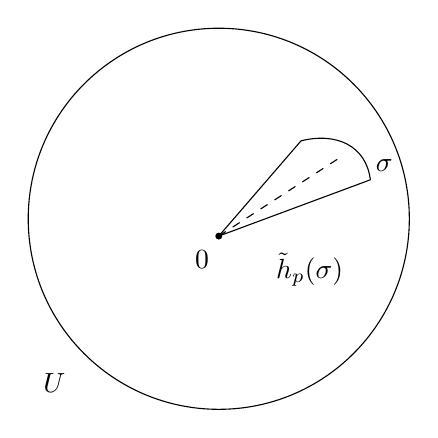
\begin{tikzpicture}[>=stealth,scale=1.1]
\draw (0,0) circle (2.2);
\node at (-1.9,-1.9) {$U$};
\fill (0,-0.2) circle (0.04); \node[below left] at (0,-0.25) {$0$};
\draw (0,-0.2) -- (0.95,0.9);
\draw (0,-0.2) -- (1.75,0.45);
\draw[dashed] (0,-0.2) -- (1.42,0.72);
\draw (0.95,0.9) .. controls (1.35,1.0) and (1.7,0.85) .. (1.75,0.45);
\node[right] at (1.7,0.62) {$\sigma$};
\node[below] at (1.05,-0.28) {$\tilde{h}_{p}(\sigma)$};
\end{tikzpicture}
\end{center}

$ \tilde{h}_{p} $ extends to a homomorphism  $ S_{p-1}(U) \to S_{p}(U) $. It follows from (18) and the \hyperref[thm:4.6]{definition 4.6}(4) of the boundary operator  $ \partial $ that

\begin{equation}
\label{eq:5.31:19}
\mathrm{i d}=\partial\circ\tilde{h}_{p+1}+\tilde{h}_{p}\circ\partial
\end{equation}

on $S_{p}(U)$ for $p \geq 1$. Before checking (19) in general, try the case in which $p = 1$, where it turns out that

\begin{equation}
\label{eq:5.31:20}
\sigma=(\tilde{h}_{2}(\sigma))^{2}-(\tilde{h}_{2}(\sigma))^{1}+(\tilde{h}_{2}(\sigma))^{0}+\tilde{h}_{1}(\sigma^{0})-\tilde{h}_{1}(\sigma^{1}),
\end{equation}

and where the corresponding picture is

\begin{center}
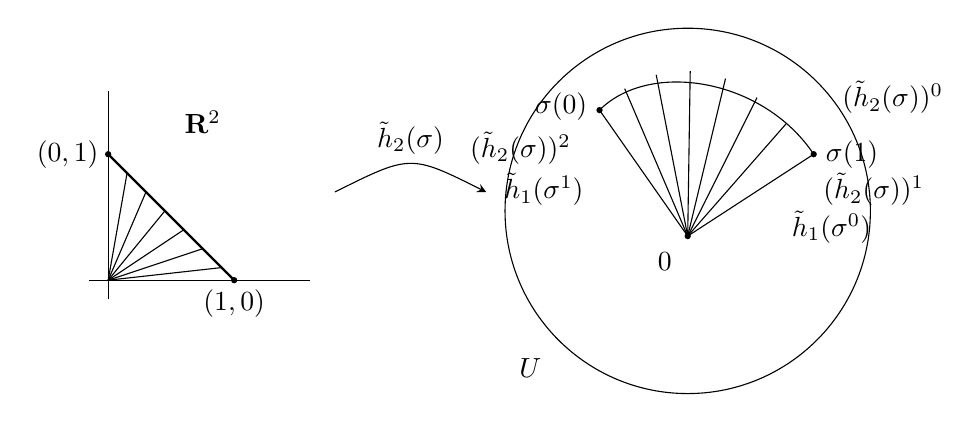
\begin{tikzpicture}[>=stealth,scale=1.6]
% left: standard 1-simplex in R^2
\draw (-0.15,0) -- (1.6,0); \draw (0,-0.15) -- (0,1.5);
\node at (0.75,1.25) {$\mathbf{R}^{2}$};
\fill (0,1) circle (0.025); \node[left] at (0,1) {$(0,1)$};
\fill (1,0) circle (0.025); \node[below] at (1,0) {$(1,0)$};
\draw[thick] (0,1) -- (1,0);
\foreach \t in {0.15,0.3,0.45,0.6,0.75,0.9}{\draw (0,0) -- (\t,{1-\t});}
\draw (0,0) -- (0,1); \draw (0,0) -- (1,0);
% arrow to right figure
\draw[->] (1.8,0.7) .. controls (2.4,1.0) .. (3.0,0.7);
\node[above] at (2.4,0.92) {$\tilde{h}_{2}(\sigma)$};
% right: cone in U
\draw (4.6,0.55) circle (1.45);
\node at (3.35,-0.7) {$U$};
\fill (4.6,0.35) circle (0.025); \node[below left] at (4.55,0.3) {$0$};
\draw (3.9,1.35) .. controls (4.3,1.75) and (5.2,1.6) .. (5.6,1.0);
\fill (3.9,1.35) circle (0.025); \node[left] at (3.88,1.38) {$\sigma(0)$};
\fill (5.6,1.0) circle (0.025); \node[right] at (5.62,1.0) {$\sigma(1)$};
\foreach \p/\q in {3.9/1.35,4.1/1.52,4.35/1.63,4.62/1.66,4.9/1.6,5.15/1.45,5.38/1.24,5.6/1.0}{\draw (4.6,0.35) -- (\p,\q);}
\node[left] at (3.75,1.05) {$(\tilde{h}_{2}(\sigma))^{2}$};
\node[left] at (3.85,0.72) {$\tilde{h}_{1}(\sigma^{1})$};
\node[right] at (5.75,1.45) {$(\tilde{h}_{2}(\sigma))^{0}$};
\node[right] at (5.6,0.72) {$(\tilde{h}_{2}(\sigma))^{1}$};
\node[right] at (5.35,0.42) {$\tilde{h}_{1}(\sigma^{0})$};
\end{tikzpicture}
\end{center}



\begin{equation}
\label{eq:5.31:21}
\tilde{h}_{p}(\sigma)(a_{1},\ldots,a_{p})=\varphi\left(\sum_{i=1}^{p}a_{i}\right)\cdot\sigma\left(a_{2}\bigg/\sum_{i=1}^{p}a_{i},\ldots,a_{p}\bigg/\sum_{i=1}^{p}a_{i}\right),
\end{equation}

where, as in (18), we assume that  $ \tilde{h}_{p}(\sigma) $ maps the origin in $\Delta^{p}$ to the origin in $U$. Now extend  $ \sigma $ to be differentiable on all of  $ \mathbb{R}^{p-1} $ so that  $ \sigma $ and each of its derivatives is bounded. Then  $ \tilde{h}_{p}(\sigma) $ is defined on all of  $ \mathbb{R}^{p} $, providing that we agree that  $ \tilde{h}_{p}(\sigma) $ maps any point where  $ \sum_{i=1}^{p} a_{i} = 0 $ to the origin in U. Moreover,  $ \tilde{h}_{p}(\sigma) $ is differentiable of class  $ C^{\infty} $ on all of  $ \mathbb{R}^{p} $. The only points where problems arise are those for which  $ \sum_{i=1}^{p} a_{i} = 0 $; and since  $ \varphi(t) $ and all of its derivatives vanish faster than any polynomial in  $ t $ as  $ t \to 0 $, and since

$\sigma$ and each of its derivatives is bounded on $\mathbb{R}^{p-1}$, it follows that all derivatives of $\tilde{h}_{p}(\sigma)$ of all orders exist, and are continuous, and are zero at points where $\sum_{i=1}^{p} a_{i}=0$. This completes the proof that (13) is a fine torsionless resolution of the constant sheaf $\mathcal{K}$, both for the continuous and for the differentiable singular theories.

Thus both resolutions (13), for the continuous and the differentiable cases, give rise, as in 5.20, to cohomology theories if we set

\begin{equation}
\label{eq:5.31:22}
\begin{aligned}{H^{q}(M,\mathcal{S})}&{{}=H^{q}\big(\Gamma\big(\mathcal{S}^{*}(M,K)\otimes\mathcal{S}\big)\big),}\\ {H^{q}(M,\mathcal{S})}&{{}=H^{q}\big(\Gamma\big(\mathcal{S}_{\infty}^{*}(M,K)\otimes\mathcal{S}\big)\big)}\\ \end{aligned}
\end{equation}

for each integer $q$ and for $\mathcal{S}$ any sheaf of $K$-modules over $M$. In view of the \hyperref[thm:5.23]{corollary of 5.23}, these theories are uniquely isomorphic and, moreover, are uniquely isomorphic with the theories \eqref{eq:5.26:11} and \eqref{eq:5.30:1}.

\subsection{\quad}\label{thm:5.32}Let $G$ be a $K$-module. We let $S^p(U,G)$ denote the $K$-module consisting of functions which assign to each singular $p$-simplex in $U$ an element of $G$. Similarly, we may replace $K$ by $G$ and $\mathcal{K}$ by the constant sheaf $\mathcal{G}$ in the constructions \eqref{eq:5.31:4}–\eqref{eq:5.31:13}.

The classical singular cohomology groups of $M$ with coefficients in a $K$-module $G$ are defined in the continuous and differentiable cases by:

\begin{equation}
\label{eq:5.32:1}
\begin{aligned}{H_{\Delta}^{q}(M;G)}&{{}=H^{q}\big(S^{*}(M,G)\big),}\\ {H_{\Delta^{\infty}}^{q}(M;G)}&{{}=H^{q}\big(S_{\infty}^{*}(M,G)\big).}\\ \end{aligned}
\end{equation}

We shall now show that the classical cohomology groups (actually K-modules) are canonically isomorphic with the sheaf cohomology modules  $H^{q}(M,\mathcal{G})$. It follows from \hyperref[thm:5.27]{Proposition 5.27} that

\begin{equation}
\label{eq:5.32:2}
0\to S_{0}^{*}(M,G)\to S^{*}(M,G)\to\Gamma\bigl(\mathcal{S}^{*}(M,G)\bigr)\to0
\end{equation}

is a short exact sequence of cochain complexes (with a similar sequence in the differentiable case). Thus if we prove that

\begin{equation}
\label{eq:5.32:3}
H^{q}\bigl(S_{0}^{*}(M,G)\bigr)=0\quad\mathrm{for\ all}\ q
\end{equation}

(also in the differentiable case), then it follows from the long exact sequence \eqref{eq:5.17:2} that there are canonical isomorphisms

\begin{equation}
\label{eq:5.32:4}
\begin{array}{r l}&{H^{q}\big(S^{*}(M,G)\big)\cong H^{q}\big(\Gamma\big(\mathcal{S}^{*}(M,G)\big)\big),}\\ &{H^{q}\big(S_{\infty}^{*}(M,G)\big)\cong H^{q}\big(\Gamma\big(\mathcal{S}_{\infty}^{*}(M,G)\big)\big).}\end{array}
\end{equation}

Thus it follows from (1) and (4), and from 5.25 (applied to the fine resolutions of $\mathcal{G}$ obtained by replacing $K$ by $G$ and $\mathcal{K}$ by $\mathcal{G}$ in \eqref{eq:5.31:13}) that we have canonical isomorphisms

\begin{equation}
\label{eq:5.32:5}
H_{\Delta}^{q}(M;G)\cong H^{q}(M,\mathcal{G})\cong H_{\Delta^{\infty}}^{q}(M;G).
\end{equation}

The proof of (3) for the continuous singular theory goes as follows. (The differentiable case is identical.) It is trivially satisfied for $q<0$ since in this range the modules of the cochain complex $S_0^*(M,G)$ are all zero. The module $S_0^*(M,G)$ is also zero since the presheaf $\{S^0(U,G); p_{U,V}\}$ is complete. Thus $H^0(S_0^*(M,G))=0$. It remains to prove (3) for $q\geq1$. Let $\mathfrak{U}=\{U_i\}$ be an arbitrary open cover of $M$. Let $S_{\mathfrak{U}}^*(M,G)$ be the cochain complex consisting of modules $S_{\mathfrak{U}}^*(M,G)$ of singular cochains $f$, with values in $G$, defined only on “$\mathfrak{U}$-small” singular $p$-simplices, that is, defined only on those singular $p$-simplices whose ranges lie in elements of $\mathfrak{U}$. Each element of $S^p(M,G)$ determines an element of $S_{\mathfrak{U}}^*(M,G)$ by restriction to $\mathcal{U}$-small simplices. The restriction homomorphisms $f_U:S^p(M,G)\to S_U^*(M,G)$ yield a surjective cochain map

\begin{equation}
\label{eq:5.32:6}
j_{\mathfrak{U}}\colon S^{*}(M,G)\to S_{\mathfrak{U}}^{*}(M,G).
\end{equation}

The kernels of the homomorphisms $j_{\mathfrak{U}}$ form a cochain complex $K_{\mathfrak{U}}^{*}$ such that

\begin{equation}
\label{eq:5.32:7}
0\to K_{\mathfrak{U}}^{*}\to S^{*}(M,G)\to S_{\mathfrak{U}}^{*}(M,G)\to0
\end{equation}

is an exact sequence of cochain complexes. The key ingredient in the proof of (3) is the fact that the cochain map $j_{\mathfrak{U}}$ induces isomorphisms in cohomology. Let us assume this for the moment. It follows from the long exact cohomology sequence for (7) that

\begin{equation}
\label{eq:5.32:8}
H^{q}(K_{\mathfrak{U}}^{*})=0\quad\mathrm{for\ all}\ q.
\end{equation}

So now let $q \geq 1$, and let $f$ be a cocycle in $S_0^q(M,G)$; that is, $df = 0$. Then, by the definition of $S_0^q(M,G)$, there is an open cover $\mathfrak{U}$ of $M$ consisting of sufficiently small open sets so that $f \in K_{\mathfrak{U}}^q$. It follows from (8) that there exists $g \in K_{\mathfrak{U}}^{q-1} \subset S_0^{q-1}(M,G)$ such that $dg = f$, which proves (3).

Now we return to the proof that the cochain map $j_{\mathfrak{U}}$ induces isomorphisms of the cohomology. Since we will work with a fixed cover $\mathfrak{U}$ of $M$, we drop the subscript $\mathfrak{U}$ from $j_{\mathfrak{U}}$. To prove that $j\colon S^{*}(M,G)\to S_{\mathfrak{U}}^{*}(M,G)$ induces isomorphisms of the cohomology modules, we shall construct a cochain map

\begin{equation}
\label{eq:5.32:9}
k\colon S_{\mathfrak{U}}^{*}(M,G)\to S^{*}(M,G)
\end{equation}

such that

\begin{equation}
\label{eq:5.32:10}
j\circ k=\mathrm{id},
\end{equation}

whence the cochain map $j$ must induce surjections of the cohomology modules, and such that there exist homotopy operators $h_{p}\colon S^{p}(M,G)\to S^{p-1}(M,G)$ for all $p$ such that

\begin{equation}
\label{eq:5.32:11}
h_{p+1}\circ d+d\circ h_{p}=\operatorname{id}-k_{p}\circ j_{p},
\end{equation}

whence  $ k \circ j $ induces the identity on cohomology, which implies that $j$ must

induce injections. Hence it will follow from (10) and (11) that $j$ induces isomorphisms on the cohomology modules. The definitions of $h$ and $k$ require a few preliminary constructions. The details become a little technical, but the general idea is this. Let $f\in S_{\mathfrak{U}}^{p}(M,G)$. Thus $f$ is defined only on $\mathfrak{U}$-small singular $p$-simplices. We want to define $k(f)$ to be an element of $S^p(M,G)$; that is, $k(f)$ is to be defined on all singular $p$-simplices. We will define an operation “subdivision” to break large singular $p$-simplices into chains of smaller ones. By subdividing any singular $p$-simplex sufficiently many times, we will obtain a chain of $\mathfrak{U}$-small singular $p$-simplices to which we can then apply $f$. So we will define $k(f)$ on the large singular simplex to be $f$ on the subdivided ones. Simplices which are already $\mathfrak{U}$-small will not be subdivided at all. The technical difficulty which arises will be due to the fact that the number of times that a singular $p$-simplex $\sigma$ needs to be subdivided in order to obtain a chain of $\mathfrak{U}$-small simplices depends on $\sigma$.

Let  $ q \geq 1 $. A linear  $ p $-simplex in  $ \Delta^q $ is a singular  $ p $-simplex of the form

\begin{equation}
\label{eq:5.32:12}
(a_{1},\ldots,a_{p})\mapsto\left(1-\sum_{i=1}^{p}a_{i}\right)v_{0}+a_{1}v_{1}+\cdots+a_{p}v_{p}
\end{equation}

$(0\mapsto v_0$ for $p=0)$, canonically determined by the ordered sequence of points $v_0,\ldots,v_p$ in $\Delta^q$. We shall denote such a linear simplex by $(v_0,\ldots,v_p)$. The identity map of $\Delta^q$ onto itself is a linear $q$-simplex in $\Delta^q$ which we shall denote simply by $\Delta^q$. The free abelian group generated by the linear $p$-simplices in $\Delta^q$ we shall denote by $L_p(\Delta^q)$. The barycenter of a linear $p$-simplicx $\sigma=(v_0,\ldots,v_p)$ in $\Delta^q$ is the point

\begin{equation}
\label{eq:5.32:13}
b_{\sigma}=\frac{1}{p+1}v_{0}+\cdots+\frac{1}{p+1}v_{p}.
\end{equation}

Given a linear $p$-simplex $\sigma = (v_0, \ldots, v_p)$ in $\Delta^q$ and a point $v \in \Delta^q$, we define the join $v\sigma$ of $v$ and $\sigma$ to be the linear $(p+1)$ simplex $(v, v_0, \ldots, v_p)$ in $\Delta^q$. The join operation extends by linearity to $L_p(\Delta^q)$. A direct calculation shows that if $p \geq 1$, then

\begin{equation}
\label{eq:5.32:14}
\partial(v\sigma)=\sigma-v(\partial\sigma).
\end{equation}

We define subdivision homomorphisms $\mathrm{Sd}: L_p(\Delta^q) \to L_p(\Delta^q)$ by setting $\mathrm{Sd} = \mathrm{id}$ for $p = 0$ and by setting

\begin{equation}
\label{eq:5.32:15}
\mathrm{Sd}(\sigma)=b_{\sigma}\mathrm{Sd}(\partial\sigma)
\end{equation}

for $\sigma$ a linear $p$-simplex in $\Delta^q$ with $p \geq 1$, and extending linearly to $L_p(\Delta^q)$. We define homomorphisms $R: L_p(\Delta^q) \to L_{p+1}(\Delta^q)$ by setting $R = 0$ for $p = 0$ and by setting

\begin{equation}
\label{eq:5.32:16}
R(\sigma)=b_{\sigma}\big(\sigma-\mathrm{Sd}(\sigma)-R(\partial\sigma)\big)
\end{equation}

for $\sigma$ a linear $p$-simplex in $\Delta^{q}$ with $p \geq 1$, and extending linearly to $L_{p}(\Delta^{q})$. It follows from (13), (14), (15), and (16), using an elementary induction argument, that

\begin{equation}
\label{eq:5.32:17}
\begin{aligned}{\partial\circ\operatorname{Sd}=\operatorname{Sd}\circ\partial,}\\ {\partial\circ R+R\circ\partial=\operatorname{id}-\operatorname{Sd}}\\ \end{aligned}
\end{equation}

on $L_{p}(\Delta^{q})$ with $p\geq1$. (The collection of modules $L_{p}(\Delta^{q})$ and homomorphisms $\partial\colon L_{p}(\Delta^{q})\to L_{p-1}(\Delta^{q})$ form what is called a chain complex in contrast with a cochain complex \eqref{eq:5.16:1} in which the homomorphisms go the other direction. The first formula in (17) says that subdivision $\mathrm{Sd}$ is a chain map of this chain complex with itself. The second formula in (17) shows that $R$ is a homotopy operator for the chain maps id and $\mathrm{Sd}$, from which it follows that $\mathrm{Sd}$ induces the identity map on the homology groups $(\ker\partial_{p}/\operatorname{Im}\partial_{p+1})$ of this chain complex.) \index{Chain complex}

We define homomorphisms $\mathbf{Sd}\colon S_p(U)\to S_p(U)$ and $R\colon S_p(U)\to S_{p+1}(U)$ for $p\geq0$ by setting

\begin{equation}
\label{eq:5.32:18}
\mathrm{Sd}(\sigma)=\sigma\circ\mathrm{Sd}(\Delta^{p}),
\end{equation}

\[
R(\sigma)=\sigma\circ R(\Delta^{p})
\]

for $\sigma$ a singular $p$-simplex in $U$, and then extending linearly to $S_{p}(U)$. It follows easily that formulas (17) hold on $S_{p}(U)$ for $p \geq 1$.

Now let  $ \sigma = (v_0, \ldots, v_p) $ be a linear  $ p $-simplex in  $ \Delta^q $. Then the diameter of each simplex of  $ \mathrm{Sd}(\sigma) $ is at most  $ p/(p+1) $ times the diameter of  $ \sigma $, for the diameter of a linear simplex  $ \sigma $ is the maximum distance between any two of the vertices  $ v_i $. Of any two vertices in a simplex in  $ \mathrm{Sd}(\sigma) $, at least one must be of the form  $ [1/(k+1)](v_{i_0} + \cdots + v_{i_k}) $ for  $ 1 \leq k \leq p $. The distance from this vertex to the other vertex is less than or equal to the distance to some  $ v_j $, and

\[
\begin{aligned}\left|\frac{1}{k+1}(v_{i_{0}}+\cdots+v_{i_{k}})-v_{j}\right|\\ =\frac{1}{k+1}\left|\sum_{l=0}^{k}(v_{i_{l}}-v_{j})\right|\leq\frac{k}{k+1}\operatorname{diam}\sigma\leq\frac{p}{p+1}\operatorname{diam}\sigma.\end{aligned}
\]

We are now ready to construct the maps $h_p$ and $k_p$. Let $\sigma$ be a singular $p$-simplex in $M$. The open cover $\sigma^{-1}(\mathfrak{U})$ of $\Delta^p$ has a Lebesgue number $\delta$ [27, p. 122]. It follows that for $s$ large enough, the diameter of each simplex in $(Sd)^s(\Delta^p)$ is less than $\delta$ where $(Sd)^s$ is the $s$-fold composition of $Sd$ with itself. Thus each singular $p$-simplex in the chain $(Sd)^s(\sigma)$ lies in an element of the cover $\Omega$. Now let $s(\sigma)$ be the smallest of those positive integers $s \geq 0$ for which each simplex of $(Sd)^s(\sigma)$ lies in an element of $\Omega$. Then we can define homomorphisms $k_p: S_l^p(M,G) \to S^p(M,G)$ by setting $k_p = id$ for $p \leq 0$, and for $p \geq 1$ by setting

\begin{equation}
\label{eq:5.32:19}
k_{p}(f)(\sigma)=f\left((\mathrm{Sd})^{s(\sigma)}(\sigma)+\sum_{j=0}^{p}(-1)^{j}R\left(\sum_{s(\sigma^{j})\leq i\leq s(\sigma)-1}(\mathrm{Sd})^{i}(\sigma^{j})\right)\right).
\end{equation}

Note that Sd raised to a negative power is to be interpreted as the zero homomorphism, and $(\mathrm{Sd})^{0}=\mathrm{id}$. We also define homomorphisms  $ h_p: S^p(M,G) \to S^{p-1}(M,G) $ by setting  $ h_p = 0 $ for  $ p \leq 1 $ and

\begin{equation}
\label{eq:5.32:20}
h_{p}(f)(\sigma)=f\left(R\left(\sum_{0\leq i\leq s(\sigma)-1}(\mathrm{Sd})^{i}(\sigma)\right)\right)
\end{equation}

for $p \geq 2$. That (10) holds is obvious, and (11) follows immediately from a straightforward calculation. Finally, the fact that the homomorphisms $k$ yield a cochain map (9) follows from (11). For from (11) we obtain

\begin{equation}
\label{eq:5.32:21}
\begin{array}{r}{d\circ k_{p}\circ j_{p}=k_{p+1}\circ j_{p+1}\circ d.}\end{array}
\end{equation}

But $j$ is a cochain map. Thus $d\circ k_{p}\circ j_{p}=k_{p+1}\circ d\circ j_{p}$. Since $j$ is surjective, it follows that $d\circ k_{p}=k_{p+1}\circ d$. This completes the proof that $j$ induces isomorphisms in cohomology.

\section{Čech Cohomology}


\subsection{\quad}\label{thm:5.33}In the Alexander-Spanier, de Rham, and singular cases we obtained a sheaf cohomology theory by exhibiting explicit fine torsionless resolutions of a constant sheaf, and we then proved that there were canonical isomorphisms of the classical cohomology modules with the sheaf cohomology modules. The Czech theory, by contrast, arises from a direct construction that does not involve finding a fine torsionless resolution of $\mathcal{K}$. We will define modules $\check{H}^{q}(M,\mathcal{S})$ for $S$ a sheaf of $K$-modules over $M$, and show that the axioms 5.18 for a cohomology theory are satisfied. We again direct your attention to the comment in the introduction to this chapter that for much of the chapter, $M$ need not be a differentiable manifold. In particular, $M$ in this section need only be a paracompact Hausdorff space.

Let $\mathfrak{U} = \{U_\alpha\}$ be an open cover of $M$. A collection $(U_0, \ldots, U_q)$ of members of the cover such that $U_0 \cap \cdots \cap U_q \neq \varnothing$ will be called a $q$-simplex. If $\sigma = (U_0, \ldots, U_q)$ is a $q$-simplex, its support $|\sigma|$ is by definition \index{Čech cohomology}

\begin{equation}
\label{eq:5.33:1}
|\sigma|=U_{0}\cap\cdots\cap U_{q}.
\end{equation}

The $i$th face of a $q$-simplex $\sigma = (U_0, \ldots, U_q)$ is the $(q-1)$ simplex $\sigma^i = (U_0, \ldots, U_{i-1}, U_{i+1}, \ldots, U_q)$. Let $C^q(\mathfrak{U},\mathcal{S})$, for $q \geq 0$, be the $K$-module consisting of functions which assign to each $q$-simplex $\sigma$ an element of $\Gamma(\mathcal{S},|\sigma|)$, and let $C^q(\mathfrak{U},\mathcal{S}) = 0$ for $q < 0$. Elements of $C^q(\mathfrak{U},\mathcal{S})$ are called $q$-cochains. With a coboundary homomorphism

\begin{equation}
\label{eq:5.33:2}
d\colon C^{q}(\mathfrak{U},\mathcal{S})\to C^{q+1}(\mathfrak{U},\mathcal{S})
\end{equation}

defined by

\begin{equation}
\label{eq:5.33:3}
d f(\sigma)=\sum_{i=0}^{q}(-1)^{i}\rho_{|\sigma|,|\sigma^{i}|}f(\sigma^{i}),
\end{equation}

one obtains a cochain complex $C^{*}(\mathfrak{U},\mathcal{S})$ whose $q$th cohomology module, which we denote by $\check{H}^{q}(\mathfrak{U},\mathcal{S})$, is called the $q$th Čech cohomology module of $(M,\mathfrak{U})$ with coefficients in $\mathcal{S}$. A homomorphism $\mathcal{S}\to\mathcal{S}'$ induces by composition a cochain map $C^{*}(\mathfrak{U},\mathcal{S})\to C^{*}(\mathfrak{U},\mathcal{S}')$ and thus induces homomorphisms

\begin{equation}
\label{eq:5.33:4}
\check{H}^{q}(\mathfrak{U},\mathcal{S})\to\check{H}^{q}(\mathfrak{U},\mathcal{S}^{\prime})
\end{equation}

for each q.

A cochain $f$ belongs to $C^0(\mathfrak{U},\mathcal{S})$ if and only if $f$ assigns to each open set $U_\alpha\in\mathfrak{U}$ a section of $\mathcal{S}$ over $U_\alpha$. $f$ is a 0-cocycle, that is $df=0$, if and only if

\begin{equation}
\label{eq:5.33:5}
0=d f(U_{\alpha_{0}},U_{\alpha_{1}})=\rho_{U_{\alpha_{0}}\cap U_{\alpha_{1}},U_{\alpha_{1}}}f(U_{\alpha_{1}})-\rho_{U_{\alpha_{0}}\cap U_{\alpha_{1}},U_{\alpha_{0}}}f(U_{\alpha_{0}})
\end{equation}

for every 1-simplex $(U_{\alpha_0}, U_{\alpha_1})$. Thus $f$ is a 0-cocycle if and only if $f$ defines a global section of $\mathcal{S}$ over $M$. Thus

\begin{equation}
\label{eq:5.33:6}
\check{H}^{0}(\mathfrak{U},\mathcal{S})=\Gamma(\mathcal{S}).
\end{equation}

We now consider the effect of refining the cover $\mathfrak{U}$. If a cover $\mathfrak{B}$ is a refinement of the cover $\mathfrak{U}$, then there exists a map $\mu\colon\mathfrak{B}\to\mathfrak{U}$ such that $V \subseteq \mu(V)$ for each $V \in \mathfrak{B}$. If $\sigma = (V_0, \ldots, V_q)$ is a $q$-simplex of the cover $\mathfrak{B}$, then we let $\mu(\sigma)$ denote the $q$-simplex $(\mu(V_0), \ldots, \mu(V_q))$ of the cover $\mathfrak{U}$. Now, $\mu$ induces a cochain map $\mu: C^*(\mathfrak{U},\mathcal{S}) \to C^*(\mathfrak{B},\mathcal{S})$ if we set

\begin{equation}
\label{eq:5.33:7}
\mu_{q}(f)(\sigma)=\rho_{|\sigma|,|\mu(\sigma)|}f\big(\mu(\sigma)\big)
\end{equation}

for $f\in C^{q}(\mathfrak{U},\mathcal{S})$ and for $\sigma$ a $q$-simplex of the cover $\mathfrak{B}$. This cochain map induces homomorphisms

\begin{equation}
\label{eq:5.33:8}
\mu_{q}^{*}\colon\check{H}^{q}(\mathfrak{U},\mathcal{S})\to\check{H}^{q}(\mathfrak{B},\mathcal{S})
\end{equation}

of the cohomology modules. We claim that if $\mu$ and $\tau$ are both refining maps of $\mathfrak{B}$ into $\mathfrak{U}$, then $\mu_{q}^{*}=\tau_{q}^{*}$ for each $q$. As usual, we prove this by finding a homotopy operator. If $\sigma=(V_{0},\ldots,V_{q-1})$ is a $(q-1)$ simplex of the cover $\mathfrak{B}$, we let

\begin{equation}
\label{eq:5.33:9}
\tilde{\sigma}_{j}=\big(\mu(V_{0}),\ldots,\mu(V_{j}),\tau(V_{j}),\ldots,\tau(V_{q-1})\big).
\end{equation}

We then define homomorphisms  $ h_{q}\colon C^{q}(\mathfrak{U},\mathcal{S})\to C^{q-1}(\mathfrak{B},\mathcal{S}) $ by setting

\begin{equation}
\label{eq:5.33:10}
h_{q}(f)(\sigma)=\sum_{j=0}^{q-1}(-1)^{j}\rho_{|\sigma|,|\widetilde{\sigma}_{j}|}f(\widetilde{\sigma}_{j}).
\end{equation}

From a straightforward calculation, one obtains

\begin{equation}
\label{eq:5.33:11}
h_{q+1}\circ d+d\circ h_{q}=\tau_{q}-\mu_{q},
\end{equation}

from which it follows that $\mu_{q}^{*}=\tau_{q}^{*}$ for each integer $q$. Thus if $\mathfrak{B}$ is a refinement of $\mathfrak{U}$, which we shall denote by $\mathfrak{B}<\mathfrak{U}$, then there are canonical homomorphisms $\check{H}^{q}(\mathfrak{U},\mathcal{S})\to\check{H}^{q}(\mathfrak{B},\mathcal{S})$. Since the set of coverings of $M$ forms a directed set under the relation $<$ of refinement, and since if $\mathfrak{S}<\mathfrak{B}<\mathfrak{U}$ then the homomorphism $\check{H}^{q}(\mathfrak{U},\mathcal{S})\to\check{H}^{q}(\mathfrak{S},\mathcal{S})$ is the composition of the $\check{H}^{q}(\mathfrak{U},\mathcal{S})\to\check{H}^{q}(\mathfrak{B},\mathcal{S})$ and $\check{H}^{q}(\mathfrak{B},\mathcal{S})\to\check{H}^{q}(\mathfrak{S},\mathcal{S})$—then the

collection of modules $\check{H}^{q}(\mathfrak{U},\mathcal{S})$ and refinement homomorphisms forms a direct system. Thus one can form the direct limit module

\begin{equation}
\label{eq:5.33:12}
\check{H}^{q}(M,\mathcal{S})=\operatorname*{dir\,lim}_{\mathfrak{U}}\check{H}^{q}(\mathfrak{U},\mathcal{S}).
\end{equation}

(Construction is completely analogous to the construction of the module $\mathcal{S}_{m}$ from the modules $S_{U}$ in 5.6.) $\check{H}^{q}(M,\mathcal{S})$ is the $q$th Čech cohomology module for $M$ with coefficients in the sheaf of $K$-modules $\mathcal{S}$. The classical $q$th Čech cohomology module $\check{H}^{q}(M;G)$ of $M$ with coefficients in a $K$-module $G$ is by definition $\check{H}^{q}(M,\mathcal{G})$, where $\mathcal{G}$ is the constant sheaf $M\times G$.

We shall now show that the Čech cohomology modules (12) give a sheaf cohomology theory in the sense of 5.18. It is apparent that  $ \check{H}^{q}(M,\mathcal{S})=0 $ for  $ q<0 $, and it follows from (6) that  $ \check{H}^{q}(M,\mathcal{S})=\Gamma(\mathcal{S}) $; thus \hyperref[thm:5.18]{5.18(a)} is satisfied. The homomorphisms (4) induced from a homomorphism  $ \mathcal{S}\to\mathcal{S}^{\prime} $ commute with the refinement homomorphisms (8) and thus induce homomorphisms

\begin{equation}
\label{eq:5.33:13}
\check{H}^{q}(M,\mathcal{S})\to\check{H}^{q}(M,\mathcal{S}^{\prime}).
\end{equation}

It is immediate that these homomorphisms satisfy \hyperref[thm:5.18]{5.18(d)} and (e).

Consider now a fine sheaf $\mathcal{S}$ and an integer $q>0$. Since every cover of $M$ has a locally finite refinement, in order to prove that $\check{H}^{q}(M,\mathcal{S}) = 0$, it suffices to prove that $\check{H}^{q}(\mathfrak{U},\mathcal{S}) = 0$ for each locally finite open cover $\mathfrak{U}$. Let $\{l_{\alpha}\}$ be a partition of unity for $\mathcal{S}$ subordinate to the locally finite open cover $\mathfrak{U} = \{U_{\alpha}\}$ of $M$. We shall define homomorphisms $h_{p}: C^{p}(U,8) \to C^{p-1}(U,8)$ for each $p \geq 1$. Let $f \in C^{p}(U,8)$, and let $\sigma = (U_{0}, \ldots, U_{p-1})$ be a $(p-1)$ simplex of the cover $U$. Then $l_{a} \circ (f(U_{0}, U_{0}, \ldots, U_{p-1}))$ has support in $U_{a} \cap U_{0} \cap \cdots \cap U_{p-1}$, so we can extend $l_{a} \circ (f(U_{a}, U_{0}, \ldots, U_{p-1}))$ to a continuous section of $8$ over $U_{0} \cap \cdots \cap U_{p-1}$ by extending it to be zero outside $U_{a} \cap U_{0} \cap \cdots \cap U_{p-1}$. We consider $I_{a} \circ (f(U_{a}, U_{0}, \ldots, U_{p-1}))$ as this section over $U_{0} \cap \cdots \cap U_{p-1}$. Now define

\begin{equation}
\label{eq:5.33:14}
h_{p}(f)(\sigma)=\sum_{\alpha}l_{\alpha}\circ\big(f(U_{\alpha},U_{0},\ldots,U_{p-1})\big).
\end{equation}

It follows that

\begin{equation}
\label{eq:5.33:15}
d\circ h_{p}+h_{p+1}\circ d=\operatorname{id}\qquad\mathrm{for}p\geq1.
\end{equation}

So if $f$ is a $q$-cocycle with $q>0$, then there is a $(q-1)$ cochain $g$, namely $g=h_q(f)$, such that $dg=f$. It follows that $\check{H}^q(\mathfrak{U},\mathcal{S})=0$. Thus axiom \hyperref[thm:5.18]{5.18(b)} is satisfied.

A short exact sheaf sequence  $ 0 \to \mathcal{S}' \to \mathcal{S} \to \mathcal{S}'' \to 0 $ induces exact sequences

\begin{equation}
\label{eq:5.33:16}
0\to C^{q}(\mathfrak{U},\mathcal{S}^{\prime})\to C^{q}(\mathfrak{U},\mathcal{S})\to C^{q}(\mathfrak{U},\mathcal{S}^{\prime\prime}).
\end{equation}

Let $\bar{C}^q(\mathfrak{U},\mathcal{S}^{\prime\prime})$ be the image of $C^q(\mathfrak{U},\mathcal{S})$ in $C^q(\mathfrak{U},\mathcal{S}^{\prime\prime})$. Then the short exact sequences

\begin{equation}
\label{eq:5.33:17}
0\to C^{q}(\mathfrak{U},\mathcal{S}^{\prime})\to C^{q}(\mathfrak{U},\mathcal{S})\to\bar{C}^{q}(\mathfrak{U},\mathcal{S}^{\prime\prime})\to0
\end{equation}

yield a short exact sequence of cochain complexes

\begin{equation}
\label{eq:5.33:18}
0\to C^{*}(\mathfrak{U},\mathcal{S}^{\prime})\to C^{*}(\mathfrak{U},\mathcal{S})\to\bar{C}^{*}(\mathfrak{U},\mathcal{S}^{\prime\prime})\to0.
\end{equation}

A refining map $\mu\colon\mathfrak{B}\to\mathfrak{U}$ induces a homomorphism of short exact sequences of cochain complexes

\begin{equation}
\label{eq:5.33:19}
\begin{aligned}{0\to C^{*}(\mathfrak{U},\mathcal{S}^{\prime})}&{{}\to C^{*}(\mathfrak{U},\mathcal{S})\to\bar{C}^{*}(\mathfrak{U},\mathcal{S}^{\prime\prime})\to0}\\ {\downarrow^{\mu}}&{{}\quad\downarrow^{\mu}\quad\downarrow^{\mu}}\\ {0\to C^{*}(\mathfrak{B},\mathcal{S}^{\prime})}&{{}\to C^{*}(\mathfrak{B},\mathcal{S})\to\bar{C}^{*}(\mathfrak{B},\mathcal{S}^{\prime\prime})\to0}\\ \end{aligned}
\end{equation}

and thus by 5.17 induces a commutative diagram of the associated cohomology sequences


\begin{equation}
\label{eq:5.33:20}
\begin{array}{c}\cdots\rightarrow\bar{H}^{q-1}(\mathfrak{U},\mathcal{S}^{\prime\prime})\xrightarrow{\partial}\check{H}^{q}(\mathfrak{U},\mathcal{S}^{\prime})\rightarrow\check{H}^{q}(\mathfrak{U},\mathcal{S})\rightarrow\bar{H}^{q}(\mathfrak{U},\mathcal{S}^{\prime\prime})\xrightarrow{\partial}\check{H}^{q+1}(\mathfrak{U},\mathcal{S}^{\prime})\rightarrow\cdots\\\big\downarrow\mu_{q-1}^{*}\quad\big\downarrow\mu_{q}^{*}\quad\big\downarrow\mu_{q}^{*}\quad\big\downarrow\mu_{q}^{*}\quad\big\downarrow\mu_{q+1}^{*}\\\cdots\rightarrow\bar{H}^{q-1}(\mathfrak{B},\mathcal{S}^{\prime\prime})\xrightarrow{\partial}\check{H}^{q}(\mathfrak{B},\mathcal{S}^{\prime})\rightarrow\check{H}^{q}(\mathfrak{B},\mathcal{S})\rightarrow\bar{H}^{q}(\mathfrak{B},\mathcal{S}^{\prime\prime})\xrightarrow{\partial}\check{H}^{q+1}(\mathfrak{B},\mathcal{S}^{\prime})\rightarrow\cdots\ .\\\end{array}
\end{equation}

On passing to the direct limit, we obtain a long exact sequence

\begin{equation}
\label{eq:5.33:21}
\begin{aligned}\cdots\longrightarrow\bar{H}^{q-1}(M,\mathcal{S}^{\prime\prime})&\xrightarrow{\partial}\check{H}^{q}(M,\mathcal{S}^{\prime})\\&\longrightarrow\check{H}^{q}(M,\mathcal{S})\longrightarrow\bar{H}^{q}(M,\mathcal{S}^{\prime\prime})\xrightarrow{\partial}\check{H}^{q+1}(M,\mathcal{S}^{\prime})\longrightarrow\cdots.\end{aligned}
\end{equation}

We shall now prove that the inclusion cochain map  $\bar{C}^*(\mathfrak{U},\mathcal{S}^{\prime\prime}) \to C^*(\mathfrak{U},\mathcal{S}^{\prime\prime})$ on passage to the direct limit in cohomology induces isomorphism

\begin{equation}
\label{eq:5.33:22}
\bar{H}^{q}(M,\mathcal{S}^{\prime\prime})\xrightarrow{\cong}\check{H}^{q}(M,\mathcal{S}^{\prime\prime}).
\end{equation}

These isomorphisms, together with (21), will then yield a long exact sequence

\begin{equation}
\label{eq:5.33:23}
\begin{aligned}\cdots\longrightarrow\check{H}^{q-1}(M,\mathcal{S}^{\prime\prime})&\xrightarrow{\partial}\check{H}^{q}(M,\mathcal{S}^{\prime})\\ \longrightarrow\check{H}^{q}(M,\mathcal{S})&\longrightarrow\check{H}^{q}(M,\mathcal{S}^{\prime\prime})\xrightarrow{\partial}\check{H}^{q+1}(M,\mathcal{S}^{\prime})\longrightarrow\cdots,\end{aligned}
\end{equation}

which proves axiom \hyperref[thm:5.18]{5.18(c)}. The quotient modules

\begin{equation}
\label{eq:5.33:24}
\bar{C}^{q}(\mathfrak{U})=C^{q}(\mathfrak{U},\mathcal{S}^{\prime\prime})/(\bar{C}^{q}(\mathfrak{U},\mathcal{S}^{\prime\prime}))
\end{equation}

together with the induced coboundary homomorphisms form a cochain complex  $\bar{C}^{*}(\mathfrak{U})$ such that

\begin{equation}
\label{eq:5.33:25}
0\to\bar{C}^{*}(\mathfrak{U},\mathcal{S}^{\prime\prime})\to C^{*}(\mathfrak{U},\mathcal{S}^{\prime\prime})\to\bar{C}^{*}(\mathfrak{U})\to0
\end{equation}

is exact. It follows from the long exact cohomology sequence for (25), upon passage to the direct limit, that (22) will follow if we prove that the direct limit of the modules  $ H^q(\widetilde{C}^*(U)) $ is 0 for all $q$. So let U be a locally finite cover of M. That the direct limit of the modules  $ H^q(\widetilde{C}^*(U)) $ is 0 will certainly follow if we prove that for an arbitrary  $ f \in C^q(U, S^*) $ there is a refinement  $ \mu: \mathfrak{B} \to U $ such that  $ \mu_q(f) \in \widetilde{C}^q(\mathfrak{B}, S^*) $. Choose a refinement  $ \mathfrak{D} = \{O_q\} $ of  $ U = \{U_q\} $ such that  $ O_q \subset U_q $ for each  $ \alpha $. For each  $ p \in M $ choose a neighborhood  $ V_p $ such that

(a)  $V_{p}\subset O_{\alpha}$ for some $\alpha$.

(b) If  $V_{p}\cap O_{\alpha}\neq\varnothing$, then $V_{p}\subset U_{\alpha}$.

(c)  $V_{p}$ lies in the intersection of the $U_{\alpha}$ containing $p$.

(d) If $\sigma$ is a $q$-simplex of the cover $\mathfrak{U}$, and $p\in|\sigma|$ (so $V_{p}\subset|\sigma|$), then $\rho_{V_{p},|\sigma|}f(\sigma)$ is the image of a section of $\mathcal{S}$ over $V_{p}$.

It is possible to satisfy (d) since there are only finitely many $q$-simplices of the cover $\mathfrak{U}$ which contain $p$. Now let $\mathfrak{B}$ be the cover $\{V_p\}$, and for every $p$ choose $O_p \in \mathfrak{U}$ and $U_p \in \mathfrak{U}$ such that $V_p \subset O_p \subset U_p$. Thus we have a refinement $\mu: \mathfrak{B} \to \mathfrak{U}$. Now let $\sigma = (V_{p_0}, \ldots, V_{p_q})$ be a $q$-simplex of the cover $\mathfrak{B}$. Then $V_{p_0} \cap O_{p_q} \neq \varnothing$, $0 \leq i \leq q$, so by (b), $V_{p_0} \subset U_{p_q}$. Thus $V_{p_0} \subset U_{p_q} \cap \cdots \cap U_{p_q} = |\mu(\sigma)|$. Therefore

\[
\begin{aligned}{\mu_{q}(f)(\sigma)}&{{}=\rho_{|\sigma|,|\mu(\sigma)|}f(U_{p_{0}},\ldots,U_{p_{q}})}\\ {}&{{}=\rho_{|\sigma|,V_{p_{0}}}\circ\rho_{V_{p_{0}},|\mu(\sigma)|}f(U_{p_{0}},\ldots,U_{p_{q}});}\\ \end{aligned}
\]

hence by condition (d),  $\mu_{q}(f)\in\bar{C}^{q}(\mathfrak{B},\mathcal{S}^{\prime\prime})$.

Finally, axiom \hyperref[thm:5.18]{5.18(f)} follows readily from the above construction of (23) by making use of \eqref{eq:5.17:3}.

Thus the Čech cohomology satisfies the axioms 5.18 for a sheaf cohomology theory.

\section{The De Rham Theorem}


\subsection{Convention}\label{thm:5.34}Since according to the \hyperref[thm:5.23]{corollary of 5.23}, any two sheaf cohomology theories on $M$ are uniquely isomorphic, we shall consider them as identified via their unique isomorphism, and shall henceforth use $H^{p}(M,8)$ to denote the $p$th cohomology module of $M$ with coefficients in the sheaf 8. With this convention,

\begin{equation}
\label{eq:5.34:1}
H^{p}(M,\mathcal{S})=\check{H}^{p}(M,\mathcal{S});
\end{equation}

and given any fine torsionless resolution

\begin{equation}
\label{eq:5.34:2}
0\to\mathcal{K}\to\mathcal{C}_{0}\to\mathcal{C}_{1}\to\mathcal{C}_{2}\to\cdots,
\end{equation}

we have

\begin{equation}
\label{eq:5.34:3}
H^{p}(M,\mathcal{S})=H^{p}\big(\Gamma(\mathcal{C}^{*}\otimes\mathcal{S})\big).
\end{equation}

\subsection{\quad}\label{thm:5.35}In the preceding sections we have obtained canonical isomorphisms

\begin{equation}
\label{eq:5.35:1}
H_{A-S}^{p}(M;G)\cong H_{\Delta}^{p}(M;G)\cong H_{\Delta^{\infty}}^{p}(M;G)\cong\check{H}^{p}(M;G)
\end{equation}

of the classical Alexander-Spanier, singular, differentiable singular, and Čech cohomology modules of a differentiable manifold $M$ with coefficients in a $K$-module $G$ over a principal ideal domain $K$. We have seen that each of these is canonically isomorphic with the sheaf cohomology module $H^{p}(M,\mathcal{G})$ with coefficients in the constant sheaf $\mathcal{G}$. If we take $K$ to be the field of real numbers, we can add the de Rham cohomology group $H_{\mathrm{de\,R}}^{p}(M)$ to the above list of isomorphisms. In particular, we have canonical isomorphisms

\begin{equation}
\label{eq:5.35:2}
H_{\mathrm{de\,R}}^{p}(M)\cong H^{p}(M,\mathcal{R})\cong H_{\Delta^{\infty}}^{p}(M;\mathbb{R}).
\end{equation}

We shall now prove, with the help of 5.24, that the explicit homomorphism from the de Rham to the differentiable singular cohomology theory obtained from integration of forms over differentiable singular simplices yields the canonical isomorphism (2).

We define homomorphisms

\begin{equation}
\label{eq:5.35:3}
k_{p}\colon E^{p}(M)\to S_{\infty}^{p}(M,\mathbb{R})
\end{equation}

for each integer  $ p \geq 0 $ by setting

\begin{equation}
\label{eq:5.35:4}
k_{p}(\omega)(\sigma)=\int_{\sigma}\omega
\end{equation}

for each differentiable $p$-form $\omega$ on $M$ and differentiable singular $p$-simplex $\sigma$ in $M$. It is an immediate consequence of Stokes' \hyperref[thm:4.7]{theorem 4.7} that the homomorphisms $k_{p}$ induce a cochain map

\begin{equation}
\label{eq:5.35:5}
k\colon E^{*}(M)\to S_{\infty}^{*}(M,\mathbb{R}).
\end{equation}

Let

\begin{equation}
\label{eq:5.35:6}
k_{p}^{*}\colon H_{\mathrm{de\,R}}^{p}(M)\to H_{\Delta^{\infty}}^{p}(M;\mathbb{R})
\end{equation}

denote the induced homomorphism of the cohomology modules (real vector spaces).  $ k_{p}^{*} $ is called the de Rham homomorphism.

\begin{theorem}{The de Rham Theorem}\label{thm:5.36}The de Rham homomorphism $k_{p}^{*}$ is the canonical isomorphism \eqref{eq:5.35:2} for each integer $p$.\end{theorem}

\begin{proof}
The homomorphisms \eqref{eq:5.35:3} can be defined for arbitrary open sets in M, and yield presheaf homomorphisms

\[
\{E^{v}(U);\rho_{U,V}\}\xrightarrow{k_{p}}\{S_{\infty}^{v}(U,\mathbb{R});\rho_{U,V}\}
\]

which commute, by Stokes' theorem, with the coboundary homomorphisms \eqref{eq:5.28:2} and \eqref{eq:5.31:10}. Thus the induced homomorphisms of the associated sheaves form a commutative diagram:

\begin{equation}
\label{eq:5.36:1}
\begin{array}{c}0\to\mathcal{R}\longrightarrow\mathcal{E}^{0}(M)\longrightarrow\mathcal{E}^{1}(M)\longrightarrow\mathcal{E}^{2}(M)\longrightarrow\cdots\\\big\downarrow\mathrm{id}\quad\big\downarrow k_{0}\quad\big\downarrow k_{1}\quad\big\downarrow k_{2}\\0\to\mathcal{R}\longrightarrow\mathcal{S}_{\infty}^{0}(M,\mathbb{R})\longrightarrow\mathcal{S}_{\infty}^{1}(M,\mathbb{R})\longrightarrow\mathcal{S}_{\infty}^{2}(M,\mathbb{R})\longrightarrow\cdots.\end{array}
\end{equation}

Consider now the following commutative diagram of cochain complexes in which the rows, according to \eqref{eq:5.30:5} and \eqref{eq:5.32:2}, are exact:

\begin{equation}
\label{eq:5.36:2}
\begin{array}{c}0\longrightarrow E^{*}(M)\xrightarrow{\text{①}}\Gamma\big(\mathcal{E}^{*}(M)\big)\longrightarrow0\\\big\downarrow k\qquad\qquad\big\downarrow\text{③}\\0\longrightarrow S_{\infty,0}^{*}(M,\mathbb{R})\longrightarrow S_{\infty}^{*}(M,\mathbb{R})\xrightarrow{\text{②}}\Gamma\big(\mathcal{S}_{\infty}^{*}(M,\mathbb{R})\big)\longrightarrow0.\end{array}
\end{equation}

The cochain map ① induces the isomorphisms $H_{\mathrm{de\,R}}^{p}(M)\cong H^{p}(M,\mathcal{R})$. We proved in \eqref{eq:5.32:4} that ② induces the isomorphisms $H_{\Delta^{\infty}}^{p}(M;\mathbb{R})\cong H^{p}(M,\mathcal{R})$. That ③ induces isomorphisms on cohomology follows from the \hyperref[thm:5.23]{corollary of 5.23} applied to the homomorphism of sheaf cohomology theories induced according to 5.24 by the homomorphism (1) of fine torsionless resolutions of $\mathcal{R}$. Thus from the uniqueness of the isomorphism between sheaf cohomology theories, ③ induces the identity isomorphism of $H^{p}(M,\mathcal{R})$. It follows that $k_{p}^{*}$ is the canonical isomorphism \eqref{eq:5.35:2} for each integer $p$.

\subsection{\quad}\label{thm:5.37}Earlier, in 4.17, we stated a slightly different version of the de Rham theorem in terms of singular homology instead of cohomology. We shall now see that there is a natural isomorphism

\begin{equation}
\label{eq:5.37:1}
H_{\Delta^{\infty}}^{p}(M;\mathbb{R})\to{}_{\infty}H_{p}(M;\mathbb{R})^{*}
\end{equation}

which composed with $k_{p}^{*}$ yields the isomorphism \eqref{eq:4.17:1}. (For the definition of the real differentiable singular homology group ${}_{\infty}H_{p}(M;\mathbb{R})$ and other relevant notation, the reader should review section 4.16.) The map (1) is defined as follows. If $f$ represents a cohomology class in $H_{\Delta^{\infty}}^{p}(M;\mathbb{R})$,

then $f$ can be considered as a linear function on the vector space ${}_{\infty}S_{p}(M;\mathbb{R})$ of real differentiable singular $p$-chains in $M$. In particular, $f$ is a linear function on the subspace of ${}_{\infty}S_{p}(M;\mathbb{R})$ consisting of the $p$-cycles, and $f$ vanishes on the $p$-boundaries in ${}_{\infty}S_{p}(M;\mathbb{R})$ since $df=0$; hence $f$ determines a linear function on the homology group ${}_{\infty}H_{p}(M;\mathbb{R})$. Since a real differentiable singular coboundary necessarily vanishes on all $p$-cycles, each cohomology class in $H_{\Delta^{\infty}}^{p}(M;\mathbb{R})$ determines a well-defined element of ${}_{\infty}H_{p}(M;\mathbb{R})^{*}$ independent of the representative $f$ chosen. This defines the map (1). We leave it to the reader as an exercise to establish that (1) is actually an isomorphism. Clearly the composition of (1) with $k_p^{*}$ is exactly the homomorphism \eqref{eq:4.17:1}. Thus \eqref{eq:4.17:1} is an isomorphism.

\end{proof}

\begin{remarks}\label{thm:5.38}
The singular cohomology groups $H_{\Delta}^{p}(M;\mathbb{R})$ are topological invariants; that is, homeomorphic spaces have isomorphic real singular cohomology (see Exercise 19). As a consequence of this and the isomorphism \eqref{eq:5.35:1} and \eqref{eq:5.35:2}, the de Rham cohomology groups are also topological invariants of a differentiable manifold.

\end{remarks}

\section{Multiplicative Structure}


In the case in which $\mathcal{S}$ is a sheaf of $K$-algebras over $M$, we shall make the direct sum of the cohomology modules $\sum H^{p}(M,\mathcal{S})$ into an associative algebra over $K$. But first we need a few preliminary constructions.

\begin{definition}\label{thm:5.39}
Let $C^*$ and ${}^{\prime}C^*$ be cochain complexes. Their tensor product $C^* \otimes {}^{\prime}C^*$ is the cochain complex whose $r$th module is the direct sum

\begin{equation}
\label{eq:5.39:1}
\sum_{p+q=r}C_{p}\otimes{}^{\prime}C_{q},
\end{equation}

and whose rth coboundary homomorphism is the direct sum

\begin{equation}
\label{eq:5.39:2}
\sum_{p+q=r}\big(d_{p}\otimes{}^{\prime}(\mathrm{id})_{q}+(-1)^{p}(\mathrm{id})_{p}\otimes{}^{\prime}d_{q}\big).
\end{equation}

If $\sigma \in Z^p(C^*)$ and $\tau \in Z^q({}^{\prime}C^*)$, then $\sigma \otimes \tau \in Z^{p+q}(C^* \otimes{}^{\prime}C^*)$; whereas if $\sigma \in B^p(C^*)$ and $\tau \in Z^q({}^{\prime}C^*)$ (or vice versa, if $\sigma \in Z^p(C^*)$ and $\tau \in B^q({}^{\prime}C^*)$), then $\sigma \otimes \tau \in B^{p+q}(C^* \otimes{}^{\prime}C^*)$. Thus there is a well-defined homomorphism

\begin{equation}
\label{eq:5.39:3}
H^{p}(C^{*})\otimes H^{q}({}^{\prime}C^{*})\to H^{p+q}(C^{*}\otimes{}^{\prime}C^{*}).
\end{equation}

\end{definition}

\begin{lemma}\label{thm:5.40}
The tensor product of two torsionless K-modules, for K a principal ideal domain, is again a torsionless K-module.

\end{lemma}

\begin{proof}
Let $\lambda \neq 0 \in K$, and let $K/\lambda$ be the $K$-module whose elements are $\{k/\lambda: k \in K\}$, and in which addition and multiplication by $K$ are defined by

\begin{equation}
\label{eq:5.40:1}
k_{1}/\lambda+k_{2}/\lambda=(k_{1}+k_{2})/\lambda,
\end{equation}

\[
k(k_{1}/\lambda)=k k_{1}/\lambda.
\]

Let A be a K-module. We define a sequence of homomorphisms

\begin{equation}
\label{eq:5.40:2}
A\to K/\lambda\otimes A\to K\otimes A\to A.
\end{equation}

The first homomorphism is defined by $a \mapsto (\lambda / \lambda) \otimes a$, the second by $\sum (k_i / \lambda) \otimes a_i \mapsto \sum k_i \otimes a_i$, and the third by $\sum k_i \otimes a_i \mapsto \sum k_i a_i$. The second homomorphism obviously has an inverse, so is an isomorphism; and the third is an isomorphism according to \eqref{eq:5.9:2}. The composition (2) sends $a \in A$ to $\lambda a \in A$. By definition, $A$ is torsionless if and only if the composition (2) has kernel zero for each $\lambda \neq 0 \in K$. Thus $A$ is torsionless if and only if

\begin{equation}
\label{eq:5.40:3}
0\to A\to(K/\lambda)\otimes A
\end{equation}

is exact for each $\lambda \neq 0 \in K$. Now let $A$ and $B$ be torsionless $K$-modules, and let $\lambda \neq 0 \in K$. Then (3) is exact, and so since $B$ is torsionless it follows from 5.14 that

\begin{equation}
\label{eq:5.40:4}
0\to A\otimes B\to(K/\lambda)\otimes A\otimes B
\end{equation}

is exact, whence $A\otimes B$ is torsionless.

\end{proof}

\begin{definition}\label{thm:5.41}
The definitions of the direct sum $\mathcal{S}\oplus\mathcal{T}$ of sheaves and the direct sum $\mathcal{S}\oplus\mathcal{T}\to\mathcal{S}^{\prime}\oplus\mathcal{T}^{\prime}$ of sheaf homomorphisms $\mathcal{S}\to\mathcal{S}^{\prime}$ and $\mathcal{T}\to\mathcal{T}^{\prime}$ are obtained by replacing $\otimes$ by $\oplus$ in $\eqref{eq:5.9:3}-(8)$, with the deletion of \eqref{eq:5.9:7}. Observe that the direct sum of fine sheaves is a fine sheaf.
\end{definition}

\subsection{The Multiplicative Structure}\label{thm:5.42}Consider a resolution

\begin{equation}
\label{eq:5.42:1}
0\to\mathcal{K}\to\mathcal{C}_{0}\xrightarrow{d_{0}}\mathcal{C}_{1}\xrightarrow{d_{1}}\mathcal{C}_{2}\xrightarrow{d_{2}}\cdots.
\end{equation}

By the tensor product of the resolution (1) with itself we mean the sequence

\begin{equation}
\label{eq:5.42:2}
\begin{aligned}{0\to\mathcal{K}\to\mathcal{C}_{0}\otimes\mathcal{C}_{0}\to(\mathcal{C}_{0}\otimes\mathcal{C}_{1})\oplus(\mathcal{C}_{1}\otimes\mathcal{C}_{0})}&{{}\to\cdots}\\ {}&{{}\cdots\to\sum_{p+q=r}\mathcal{C}_{p}\otimes\mathcal{C}_{q}\to\cdots}\\ \end{aligned}
\end{equation}

in which the homomorphism $\mathcal{K}\to\mathcal{C}_{0}\otimes\mathcal{C}_{0}$ is the composition $\mathcal{K}\cong\mathcal{K}\otimes\mathcal{K}\to\mathcal{C}_{0}\otimes\mathcal{C}_{0}$, and in which the homomorphism whose domain is $\sum_{p+q=r}\mathcal{C}_{p}\otimes\mathcal{C}_{q}$ is the direct sum

\begin{equation}
\label{eq:5.42:3}
\sum_{p+q=r}\bigl(d_{p}\otimes(\mathrm{id})_{q}+(-1)^{p}(\mathrm{id})_{p}\otimes d_{q}\bigr).
\end{equation}

If (1) is a fine torsionless resolution of $\mathcal{K}$, we claim that (2) is also a fine torsionless resolution of $\mathcal{K}$. That the sheaves in (2) are fine is a consequence of the fact that tensor products and direct sums of fine sheaves are also fine sheaves. From 5.40 and the observation that direct sums of torsionless $K$-modules are torsionless, it follows that the sheaves in (2) are torsionless. That (2) is exact, therefore a resolution, is easily seen at $\mathcal{K}$ and at $\mathcal{C}_0 \otimes \mathcal{C}_0$, and is proved elsewhere by applying the Kunneth formula to the cochain complexes obtained for each $m \in M$ from

\begin{equation}
\label{eq:5.42:4}
\begin{aligned}\cdots\to0\to\mathcal{C}_{0}\otimes\mathcal{C}_{0}\to(\mathcal{C}_{0}\otimes\mathcal{C}_{1})\oplus(\mathcal{C}_{1}&\otimes\mathcal{C}_{0})\to\cdots\\&\cdots\to\sum_{p+q=r}\mathcal{C}_{p}\otimes\mathcal{C}_{q}\to\cdots\end{aligned}
\end{equation}

by restricting to the stalks over $m$. The extensive algebra necessary for a proof of the Kunneth formula, which expresses the cohomology of the tensor product of cochain complexes in terms of the cohomology of the individual complexes, would not be particularly illuminating for our purposes, so we shall simply refer the interested reader to Spanier [28, Ch. 5, §4, THEOREM 2], where the Kunneth formula is proved in detail.

Let $\mathcal{S}$ be a sheaf over $M$. From the resolution (2) we obtain as in \eqref{eq:5.19:2} a cochain complex which we shall denote by $\Gamma(\mathcal{C}^*\otimes\mathcal{C}^*\otimes\mathcal{S})$. If $\mathcal{S}$ is a sheaf of algebras over $M$, then the natural homomorphism $\mathcal{S}\otimes\mathcal{S}\to\mathcal{S}$ determined by the multiplicative structure of the stalks induces homomorphisms

\begin{equation}
\label{eq:5.42:5}
\Gamma(\mathcal{C}_{p}\otimes\mathcal{S})\otimes\Gamma(\mathcal{C}_{{q}}\otimes\mathcal{S})\to\Gamma(\mathcal{C}_{{p}}\otimes\mathcal{C}_{{q}}\otimes\mathcal{S}\otimes\mathcal{S})\to\Gamma(\mathcal{C}_{{p}}\otimes\mathcal{C}_{{q}}\otimes\mathcal{S})
\end{equation}

which in turn induce a cochain map

\begin{equation}
\label{eq:5.42:6}
\Gamma(\mathcal{C}^{*}\otimes\mathcal{S})\otimes\Gamma(\mathcal{C}^{*}\otimes\mathcal{S})\to\Gamma(\mathcal{C}^{*}\otimes\mathcal{C}^{*}\otimes\mathcal{S}).
\end{equation}

We have, according to \eqref{eq:5.39:3}, a well-defined homomorphism

\begin{equation}
\label{eq:5.42:7}
H^{p}(M,\mathcal{S})\otimes H^{q}(M,\mathcal{S})\to H^{p+q}\big(\Gamma(\mathcal{C}^{*}\otimes\mathcal{S})\otimes\Gamma(\mathcal{C}^{*}\otimes\mathcal{S})\big).
\end{equation}

In the case in which 8 is a sheaf of algebras over M, the cochain map (6) induces, together with (7), a homomorphism

\begin{equation}
\label{eq:5.42:8}
H^{p}(M,\mathcal{S})\otimes H^{q}(M,\mathcal{S})\to H^{p+q}(M,\mathcal{S}).
\end{equation}

This will define the multiplicative structure in sheaf cohomology. But first we need to show that the multiplication defined by (8) is independent of the resolution (1) with which we began. Consider another fine torsionless resolution

\begin{equation}
\label{eq:5.42:9}
0\to\mathcal{H}\to\widetilde{\mathcal{C}}_{0}\to\widetilde{\mathcal{C}}_{1}\to\widetilde{\mathcal{C}}_{2}\to\cdots.
\end{equation}

By tensoring the resolution (1) with the resolution (9) (construction completely analogous to the tensor product of (1) with itself given in (2) and (3)),

we obtain another fine torsionless resolution

\begin{equation}
\label{eq:5.42:10}
\begin{aligned}{0\to\mathcal{K}\to\mathcal{C}_{0}\otimes\widetilde{\mathcal{C}}_{0}\to(\mathcal{C}_{0}\otimes\widetilde{\mathcal{C}}_{1})\oplus(\mathcal{C}_{1}\otimes\widetilde{\mathcal{C}}_{0})}&{{}\to\cdots}\\ {}&{{}\cdots\to\sum_{p+q=r}\mathcal{C}_{p}\otimes\widetilde{\mathcal{C}}_{q}\to\cdots.}\\ \end{aligned}
\end{equation}

A homomorphism of the resolution (1) to the resolution (10), in the sense of 5.24, is generated by the homomorphisms

\begin{equation}
\label{eq:5.42:11}
\mathcal{C}_{p}\cong\mathcal{C}_{p}\otimes\mathcal{K}\to\mathcal{C}_{p}\otimes\widetilde{\mathcal{C}}_{0}\to\sum_{r+s=p}\mathcal{C}_{r}\otimes\widetilde{\mathcal{C}}_{s},
\end{equation}

where the last map is inclusion. This homomorphism of resolutions induces a cochain map $\Gamma(\mathcal{C}^* \otimes \mathcal{S}) \to \Gamma(\mathcal{C}^* \otimes \widetilde{\mathcal{C}}^* \otimes \mathcal{S})$ which, according to 5.24 and the \hyperref[thm:5.23]{corollary of 5.23}, induces the identity map $H^q(M, \mathcal{S}) \to H^q(M, \mathcal{S})$. By applying these constructions to various resolutions and then tensoring resulting cochain complexes, one obtains a commutative diagram of cochain complexes and cochain maps

\begin{equation}
\label{eq:5.42:12}
\begin{array}{c}\Gamma(\mathcal{C}^{*}\otimes\mathcal{S})\quad\otimes\Gamma(\mathcal{C}^{*}\otimes\mathcal{S})\quad\xrightarrow{\quad\quad\quad}\Gamma(\mathcal{C}^{*}\otimes\mathcal{C}^{*}\otimes\mathcal{S})\\\downarrow\quad\downarrow\\\Gamma(\mathcal{C}^{*}\otimes\widetilde{\mathcal{C}}^{*}\otimes\mathcal{S})\otimes\Gamma(\mathcal{C}^{*}\otimes\widetilde{\mathcal{C}}^{*}\otimes\mathcal{S})\xrightarrow{\quad\quad\quad}\Gamma(\mathcal{C}^{*}\otimes\widetilde{\mathcal{C}}^{*}\otimes\mathcal{C}^{*}\otimes\widetilde{\mathcal{C}}^{*}\otimes\mathcal{S})\\\uparrow\quad\uparrow\\\Gamma(\widetilde{\mathcal{C}}^{*}\otimes\mathcal{S})\otimes\Gamma(\widetilde{\mathcal{C}}^{*}\otimes\mathcal{S})\quad\xrightarrow{\quad\quad\quad}\Gamma(\widetilde{\mathcal{C}}^{*}\otimes\widetilde{\mathcal{C}}^{*}\otimes\mathcal{S})\\\end{array}
\end{equation}

from which is induced the following commutative diagram on cohomology:

\begin{center}
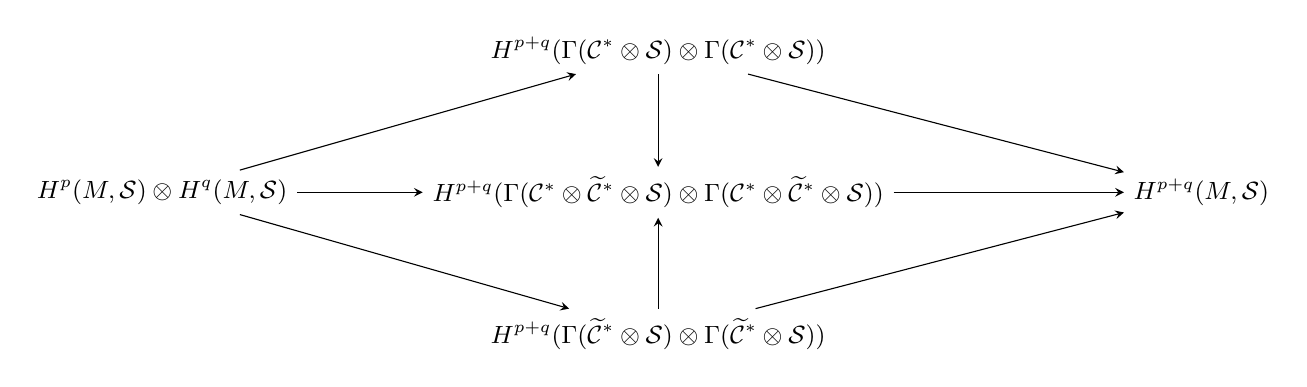
\begin{tikzpicture}[>=stealth,every node/.style={font=\small}]
\node (ML) at (0,0) {$H^{p}(M,\mathcal{S})\otimes H^{q}(M,\mathcal{S})$};
\node (T) at (6.3,1.8) {$H^{p+q}(\Gamma(\mathcal{C}^{*}\otimes\mathcal{S})\otimes\Gamma(\mathcal{C}^{*}\otimes\mathcal{S}))$};
\node (MC) at (6.3,0) {$H^{p+q}(\Gamma(\mathcal{C}^{*}\otimes\widetilde{\mathcal{C}}^{*}\otimes\mathcal{S})\otimes\Gamma(\mathcal{C}^{*}\otimes\widetilde{\mathcal{C}}^{*}\otimes\mathcal{S}))$};
\node (B) at (6.3,-1.8) {$H^{p+q}(\Gamma(\widetilde{\mathcal{C}}^{*}\otimes\mathcal{S})\otimes\Gamma(\widetilde{\mathcal{C}}^{*}\otimes\mathcal{S}))$};
\node (MR) at (13.2,0) {$H^{p+q}(M,\mathcal{S})$};
\draw[->] (ML) -- (T);
\draw[->] (ML) -- (MC);
\draw[->] (ML) -- (B);
\draw[->] (T) -- (MC);
\draw[->] (B) -- (MC);
\draw[->] (T) -- (MR);
\draw[->] (MC) -- (MR);
\draw[->] (B) -- (MR);
\end{tikzpicture}
\end{center}

From (12) it follows that the multiplicative structure (8) is independent of the choice of (1).

It follows from the construction of (8) and the associativity of tensor products that the multiplicative structure induced on $\sum_{p} H^{p}(M,\mathcal{S})$ by (8) is associative. Thus (8) makes $\sum_{p} H^{p}(M,\mathcal{S})$ into an associative algebra over $K$.

The homomorphisms  $ \mathcal{C}_{p} \otimes \mathcal{C}_{q} \to \mathcal{C}_{q} \otimes \mathcal{C}_{p} $ defined by  $ c_{p} \otimes c_{q} \to (-1)^{pq} c_{q} \otimes c_{p} $ induce a homomorphism of the resolution (2) with itself in the sense of 5.24. According to 5.24, this homomorphism of (2) induces a homomorphism of cohomology theories which by the \hyperref[thm:5.23]{corollary of 5.23} must

be the identity isomorphism. But the induced homomorphism  $ H^{p+q}(M,\mathcal{S}) \to H^{p+q}(M,\mathcal{S}) $ sends  $ u \cdot v $ into  $ (-1)^{pq}v \cdot u $ if  $ u \in H^p(M,\mathcal{S}) $ and  $ v \in H^q(M,\mathcal{S}) $. Thus the multiplicative structure of  $ \sum_p H^p(M,\mathcal{S}) $ satisfies the anti-commutative relation

\begin{equation}
\label{eq:5.42:13}
u\cdot v=(-1)^{p q}v\cdot u\qquad\big(u\in H^{p}(M,\mathcal{S});v\in H^{q}(M,\mathcal{S})\big).
\end{equation}

\subsection{The de Rham Cohomology Algebra}\label{thm:5.43}Exterior multiplication of differential forms induces, by mapping  $ \sigma \otimes \alpha \mapsto \sigma \wedge \alpha $, a cochain map

\begin{equation}
\label{eq:5.43:1}
E^{*}(M)\otimes E^{*}(M)\xrightarrow{\wedge}E^{*}(M)
\end{equation}

which together with the natural homomorphisms

\begin{equation}
\label{eq:5.43:2}
H_{\mathrm{de\,R}}^{p}(M)\otimes H_{\mathrm{de\,R}}^{q}(M)\to H^{p+q}\big(E^{\ast}(M)\otimes E^{\ast}(M)\big)
\end{equation}

of \eqref{eq:5.39:3} induces homomorphisms

\begin{equation}
\label{eq:5.43:3}
H_{\mathrm{de\,R}}^{p}(M)\otimes H_{\mathrm{de\,R}}^{q}(M)\to H_{\mathrm{de\,R}}^{p+q}(M),
\end{equation}

which make the direct sum $\sum_{p} H_{\mathrm{de\,R}}^{p}(M)$ into an associative algebra over $\mathbb{R}$. This is the classical multiplicative structure in de Rham cohomology. Now, $\sum_{p} H_{\mathrm{de\,R}}^{p}(M)$ also inherits an associative algebra structure from the algebra structure \eqref{eq:5.42:8} in sheaf cohomology via the canonical isomorphism

\[
\sum_{p}H_{\mathrm{de\,R}}^{p}(M)\cong\sum_{p}H^{p}(M,\mathcal{R}).
\]

We shall now prove that these two algebra structures on $\sum_{p} H_{\mathrm{de\,R}}^{p}(M)$ are identical. For each open set $U \subset M$, exterior multiplication induces homomorphisms

\begin{equation}
\label{eq:5.43:4}
E^{p}(U)\otimes E^{q}(U)\to E^{p+q}(U)
\end{equation}

which commute with appropriate restrictions and thus yield presheaf homomorphisms

\begin{equation}
\label{eq:5.43:5}
\left\{E^{p}(U);\rho_{U,V}\right\}\otimes\left\{E^{q}(U);\rho_{U,V}\right\}\to\left\{E^{p+q}(U);\rho_{U,V}\right\}
\end{equation}

which in turn induce sheaf homomorphisms

\begin{equation}
\label{eq:5.43:6}
\mathcal{E}^{p}(M)\otimes\mathcal{E}^{q}(M)\to\mathcal{E}^{p+q}(M).
\end{equation}

The homomorphisms (6) induce, as is easily checked, a homomorphism (in the sense of 5.24) of the tensor product of the resolution \eqref{eq:5.28:3} with itself into itself:

\begin{equation}
\label{eq:5.43:7}
\begin{array}{c}0\to\mathcal{R}\to\mathcal{E}^{0}(M)\otimes\mathcal{E}^{0}(M)\to(\mathcal{E}^{0}(M)\otimes\mathcal{E}^{1}(M))\oplus(\mathcal{E}^{1}(M)\otimes\mathcal{E}^{0}(M))\to\cdots\\\big\downarrow\mathrm{id}\qquad\big\downarrow\qquad\qquad\big\downarrow\\0\to\mathcal{R}\longrightarrow\mathcal{E}^{0}(M)\longrightarrow\mathcal{E}^{1}(M)\longrightarrow\cdots\end{array}
\end{equation}

The homomorphism (7) induces a cochain map $\Gamma(\mathcal{E}^*(M)\otimes\mathcal{E}^*(M))\to\Gamma(\mathcal{E}^*(M))$ which, according to 5.24 and the \hyperref[thm:5.23]{corollary of 5.23}, induces the identity map $H^q(M,\mathcal{R})\to H^q(M,\mathcal{R})$. Consider now the following commutative diagram of cochain complexes:

\begin{equation}
\label{eq:5.43:8}
\begin{matrix}\Gamma\big(\mathcal{E}^{*}(M)\big)\otimes\Gamma\big(\mathcal{E}^{*}(M)\big)\to\Gamma\big(\mathcal{E}^{*}(M)\otimes\mathcal{E}^{*}(M)\big)\to\Gamma\big(\mathcal{E}^{*}(M)\big)\\\uparrow\quad\uparrow\\E^{*}(M)\otimes E^{*}(M)\longrightarrow E^{*}(M)\end{matrix}
\end{equation}

The diagram (8), together with \eqref{eq:5.39:3}, induces the following commutative diagram on cohomology:

\[
\begin{array}{c}H^{p}(M,\mathcal{R})\otimes H^{q}(M,\mathcal{R})\to H^{p+q}\big(\Gamma\big(\mathcal{E}^{*}(M)\big)\otimes\Gamma\big(\mathcal{E}^{*}(M)\big)\big)\to H^{p+q}(M,\mathcal{R})\xrightarrow{\mathrm{id}}H^{p+q}(M,\mathcal{R})\\\big\uparrow\qquad\qquad\big\uparrow\qquad\qquad\big\uparrow\\H_{\mathrm{de\,R}}^{p}(M)\otimes H_{\mathrm{de\,R}}^{q}(M)\longrightarrow H^{p+q}\big(E^{*}(M)\otimes E^{*}(M)\big)\longrightarrow H_{\mathrm{de\,R}}^{p+q}(M).\end{array}
\]

The composition of homomorphisms in the top row of (9) gives precisely the multiplicative structure \eqref{eq:5.42:8} in sheaf cohomology; whereas the composition in the bottom row of (9) is precisely the classical multiplicative structure (2), and the first and last vertical arrows are the canonical isomorphisms. Thus the classical algebra structure on $\sum H_{d \cdot R}^{p}(M)$ is identical with that induced from the algebra structure on sheaf cohomology.

\subsection{The Singular Cohomology Algebra}\label{thm:5.44}This section will be written in terms of the continuous singular cohomology. All considerations, however, apply in exactly the same manner to the differentiable singular theory. Let $f\in S^{p}(M,K)$ be a singular $p$-cochain, and let $g\in S^{q}(M,K)$ be a singular $q$-cochain. We shall define a singular  $ (p+q) $ cochain  $ f \to g $ called the cup product of f and g. Let  $ \sigma $ be a singular  $ (p+q) $ simplex in M. Define

\begin{equation}
\label{eq:5.44:1}
\begin{aligned}{}&{{}(f\smallsmile g)(\sigma)}\\ {}&{{}\quad=f(\sigma\circ k_{p+q}^{p+q-1}\circ k_{p+q-1}^{p+q-2}\circ\cdots\circ k_{p+1}^{p})g(\sigma\circ k_{0}^{p+q-1}\circ k_{0}^{p+q-2}\circ\cdots\circ k_{0}^{q}),}\\ \end{aligned}
\end{equation}

where if $q=0$, then the first factor on the right-hand side of (1) is $f(\sigma)$; and if $p=0$, then the second factor on the right-hand side of (1) is $g(\sigma)$. The $k$'s are the mappings defined in \eqref{eq:4.6:2}. In other words, (1) says that we start with $\sigma$ and take the top face $q$ times to get a $p$-simplex to which we apply $f$, and we start with $\sigma$ and take the 0-face $p$ times to get a $q$-simplex to which we apply $g$. The multiplication on the right-hand side of (1) takes place in the principal ideal domain $K$. Associativity, namely,

\begin{equation}
\label{eq:5.44:2}
f\smallsmile(g\smallsmile h)=(f\smallsmile g)\smallsmile h,
\end{equation}

follows from (1) and from the identity

\begin{equation}
\label{eq:5.44:3}
\begin{aligned}{k_{0}^{p+q+r-1}\circ\cdots\circ k_{0}^{q+r}\circ k_{q+r}^{q+r-1}}&{{}\circ\cdots\circ k_{q+1}^{q}}\\ {}&{{}=k_{p+q+r}^{p+q+r-1}\circ\cdots\circ k_{p+q+1}^{p+q}\circ k_{0}^{p+q-1}\circ\cdots\circ k_{0}^{q}}\\ \end{aligned}
\end{equation}

which follows from repeated applications of \eqref{eq:4.6:5}. The bilinear map  $(f,g)\mapsto f\smallsmile g$ induces a homomorphism

\begin{equation}
\label{eq:5.44:4}
S^{p}(M,K)\otimes S^{q}(M,K)\to S^{p+q}(M,K).
\end{equation}

We claim that

\begin{equation}
\label{eq:5.44:5}
(df)\smallsmile g+(-1)^{p}f\smallsmile(dg)=d(f\smallsmile g).
\end{equation}

We suggest that the reader check (5) first for the case in which $f$ and $g$ are 1-cochains and $\sigma$ is a 3-simplex. In this case some simple pictures will aid in following the computation. In general, let $\tau$ be a singular $(p+q+1)$ simplex. Then from (1) and \eqref{eq:5.31:8}, and from repeated applications of \eqref{eq:4.6:5}, we obtain

\[
\begin{aligned}{d(f\smallsmile g)(\tau)}&{{}=\sum_{l=0}^{p+q+1}(-1)^{l}(f\smallsmile g)(\tau\circ k_{l}^{p+q})}\\ {=\sum_{l=0}^{p+q+1}}&{{}(-1)^{l}f(\tau\circ k_{l}^{p+q}\circ k_{p+q}^{p+q-1}\circ\cdots\circ k_{p+1}^{p})\;g(\tau\circ k_{l}^{p+q}\circ k_{0}^{p+q-1}\circ\cdots\circ k_{0}^{q})}\\ {=\sum_{l=0}^{p}}&{{}(-1)^{l}f(\tau\circ k_{l}^{p+q}\circ k_{p+q}^{p+q-1}\circ\cdots\circ k_{p+1}^{p})\;g(\tau\circ k_{0}^{p+q}\circ\cdots\circ k_{0}^{q})}\\ {}&{{}+\sum_{l=p+1}^{p+q+1}(-1)^{l}f(\tau\circ k_{p+q+1}^{p+q}\circ\cdots\circ k_{p+1}^{p})\;g(\tau\circ k_{0}^{p+q}\circ\cdots\circ k_{l-p}^{q+1}\circ k_{l-p}^{q})}\\ {=\sum_{l=0}^{p}}&{{}(-1)^{l}f(\tau\circ k_{p+q+1}^{p+q}\circ k_{p+q}^{p+q-1}\circ\cdots\circ k_{p+2}^{p+1}\circ k_{l}^{p})\;g(\tau\circ k_{0}^{p+q}\circ\cdots\circ k_{0}^{q})}\\ {}&{{}+(-1)^{p}f(\tau\circ k_{p+q+1}^{p+q}\circ\cdots\circ k_{p+1}^{p})\sum_{j=1}^{q+1}(-1)^{j}g(\tau\circ k_{0}^{p+q}\circ\cdots\circ k_{0}^{q+1}\circ k_{j}^{q})}\\ {=\sum_{l=0}^{p+1}}&{{}(-1)^{l}f(\tau\circ k_{p+q+1}^{p+q}\circ k_{p+q}^{p+q-1}\circ\cdots\circ k_{p+2}^{p+1}\circ k_{1}^{p})\;g(\tau\circ k_{0}^{p+q}\circ\cdots\circ k_{0}^{q})}\\ {}&{{}+(-1)^{p}f(\tau\circ k_{p+q+1}^{p+q}\circ\cdots\circ k_{p+1}^{p})\sum_{j=0}^{q+1}(-1)^{j}g(\tau\circ k_{0}^{p+q}\circ\cdots\circ k_{0}^{q+1}\circ k_{j}^{q})}\\ {}\\ {}&{{}=(d f\smallsmile g)(\tau)+(-1)^{p}(f\smallsmile d g)(\tau).}\\ \end{aligned}
\]

It follows from (5) that the homomorphisms (4) determine a cochain map

\begin{equation}
\label{eq:5.44:6}
S^{*}(M,K)\otimes S^{*}(M,K)\to S^{*}(M,K).
\end{equation}

The cochain map (6) together with the natural homomorphisms

\begin{equation}
\label{eq:5.44:7}
H_{\Delta}^{p}(M;K)\otimes H_{\Delta}^{q}(M;K)\to H^{p+q}\big(S^{*}(M,K)\otimes S^{*}(M,K)\big)
\end{equation}

of \eqref{eq:5.39:3} induces homomorphisms

\begin{equation}
\label{eq:5.44:8}
H_{\Delta}^{p}(M;K)\otimes H_{\Delta}^{q}(M;K)\to H_{\Delta}^{p+q}(M;K)
\end{equation}


which give the direct sum  $\sum_{p} H_{\Delta}^{p}(M;K)$ the structure of an associative algebra over $K$. This is the classical multiplicative structure of singular cohomology. Now, $\sum_{p} H_{\Delta}^{p}(M;K)$ also inherits an associative algebra structure from the algebra structure \eqref{eq:5.42:8} on sheaf cohomology via the canonical isomorphism $\sum_{p} H_{\Delta}^{p}(M;K)\cong\sum_{p} H_{\Delta}^{p}(M,\mathcal{K})$. The proof that these two algebra structures on $\sum_{p} H_{\Delta}^{p}(M;K)$ are identical is exactly the same as the proof of the corresponding statement for the de Rham cohomology as given in \eqref{eq:5.43:4} through (9), but with the replacement of $\mathcal{E}^{*}(M)$ by $\mathcal{S}^{*}(M,K)$ and $E^{*}(M)$ by $S^{*}(M,K)$, and so on.

The results of 5.43 and 5.44 provide the following more complete version of the de Rham \hyperref[thm:5.36]{theorem 5.36}.

\begin{theorem}{The de Rham Theorem}\label{thm:5.45}The de Rham homomorphism

\begin{equation}
\label{eq:5.45:1}
k^{*}\colon\sum_{p}H_{\mathrm{de\,R}}^{p}(M)\to\sum_{p}H_{\Delta^{\infty}}^{p}(M;\mathbb{R})
\end{equation}

is an algebra isomorphism.
\end{theorem}

\section{Supports}


\subsection{\quad}\label{thm:5.46}A family of supports on $M$ is a family $\Phi$ of closed subsets of $M$ satisfying:

(a) The union of any two members of $\Phi$ is again in $\Phi$. \index{Family of supports}

(b) Any closed subset of a member of $\Phi$ is also a member of $\Phi$.

(c) Each member of  $ \Phi $ has a neighborhood whose closure is in  $ \Phi $.

Let $\Phi$ be a family of supports on $M$. We recall that $M$ is assumed to be at least a paracompact Hausdorff space and where necessary is actually a differentiable manifold. If $\mathcal{S}$ is a sheaf over $M$, we let $\Gamma_{\Phi}(\mathcal{S})$ be the set of sections of $\mathcal{S}$ whose supports are members of $\Phi$. It follows from condition (a) that $\Gamma_{\Phi}(\mathcal{S})$ is a submodule of $\Gamma(\mathcal{S})$. It follows from (b) that a sheaf homomorphism $\mathcal{S}\to\mathcal{S}'$ induces a homomorphism $\Gamma_{\Phi}(\mathcal{S})\to\Gamma_{\Phi}(\mathcal{S}')$.

\hyperref[thm:5.12]{Theorem 5.12} has an exact analog with supports. One needs only to make a slight modification in the proof by using condition (c) to help choose a cover which will guarantee that the resulting section of $\mathcal{S}$ actually lies in $\Gamma_{\Phi}(\mathcal{S})$. The details are left to the reader as an exercise.

A cohomology theory $\mathcal{H}_{\Phi}$ for $M$ with supports $\Phi$ and with coefficients in sheaves of $K$-modules over $M$ is defined exactly as in 5.18, with the exceptions that $\Gamma(\mathcal{S})$ is replaced by $\Gamma_{\Phi}(\mathcal{S})$ in \hyperref[thm:5.18]{5.18(a)} and the cohomology modules are now denoted by ${}_{\Phi}H^{p}(M,\mathcal{S})$. The entire development of this chapter can be carried through for cohomology with supports with very few modifications. We shall briefly sketch those modifications.

The proof of existence and uniqueness of a cohomology theory with supports (which will make use of the support version of \hyperref[thm:5.12]{Theorem 5.12}) proceeds as in 5.18 through 5.25 with the exception that when given a fine torsionless resolution $0\to\mathcal{K}\to\mathcal{C}_0\to\mathcal{C}_1\to\mathcal{C}_2\to\cdots$, we now define the sheaf cohomology modules by setting

\begin{equation}
\label{eq:5.46:1}
{}_{\Phi}H^{q}(M,\mathcal{S})=H^{q}\big(\Gamma_{\Phi}(\mathcal{C}^{*}\otimes\mathcal{S})\big).
\end{equation}

Let $\{S_U; \rho_{U,V}\}$ be a presheaf with associated sheaf $\mathcal{S}$. We let ${}_{\Phi}S_{M}$ be the submodule of $S_{M}$ consisting of those elements mapping into $\Gamma_{\Phi}(\mathcal{S})$ under the canonical homomorphism $S_{M}\to\Gamma(\mathcal{S})$. It then follows from \hyperref[thm:5.27]{Proposition 5.27} and the definition of ${}_{\Phi}S_{M}$ that 5.27 holds if we replace \eqref{eq:5.27:2} by

\begin{equation}
\label{eq:5.46:2}
0\to(S_{M})_{0}\to{}_{\Phi}S_{M}\to\Gamma_{\Phi}(\mathcal{S})\to0.
\end{equation}

The classical cohomology theories with supports are defined by:

\begin{equation}
\label{eq:5.46:3}
\begin{aligned}{}_{\Phi}H_{A-S}^{q}(M;G)&=H^{q}\big({}_{\Phi}A^{*}(M,G)/A_{0}^{*}(M,G)\big),\\ {}_{\Phi}H_{\mathrm{de\,R}}^{q}(M)&=H^{q}\big({}_{\Phi}E^{*}(M)\big),\\ {}_{\Phi}H_{\Delta}^{q}(M;G)&=H^{q}\big({}_{\Phi}S^{*}(M,G)\big),\\ {}_{\Phi}H_{\Delta^{\infty}}^{q}(M;G)&=H^{q}\big({}_{\Phi}S_{\infty}^{*}(M,G)\big).\end{aligned}
\end{equation}

In the Čech theory, the support of a $q$-cochain $f\in C^{q}(\mathfrak{U},\mathcal{S})$ is by definition the union of the supports of the sections $f(\sigma)$ as $\sigma$ runs over the $q$-simplices of the cover $\mathfrak{U}$. If we set ${}_{\Phi}C^{q}(\mathfrak{U},\mathcal{S})$ equal to the module of $q$-cochains with supports in $\Phi$, then the development of the Čech theory proceeds as before and yields the Čech cohomology modules ${}_{\Phi}\check{H}^{q}(M,\mathcal{S})$ with supports.

The resultant cohomology theories will depend on the family of supports chosen. Ordinary cohomology is the same as the special case of cohomology with supports in which $\Phi$ is taken to be the family of all closed sets.

The isomorphism theorems and the development of the multiplicative structure all proceed for supports exactly as before. In particular, we have the de Rham theorem with supports:

\begin{equation}
\label{eq:5.46:4}
k^{*}\colon\sum_{p}{}_{\Phi}H_{\mathrm{de\,R}}^{p}(M)\cong\sum_{p}{}_{\Phi}H_{\Delta^{\infty}}^{p}(M;\mathbb{R})
\end{equation}

is an algebra isomorphism.

\section{Exercises}

\begin{problemset}

\item Let $\mathcal{S}$ be a sheaf over $M$. Prove that the mapping  $ m \mapsto 0 \in \mathcal{S}_m $ (the “0-section”) is continuous.

\item Prove that sections of sheaves are local homeomorphisms and therefore are open maps.

\item Prove that if two sections of a sheaf agree at one point, then they agree on a neighborhood of that point. Conclude that the set of points on which a section is not zero is a closed set.

\item A $C^{\infty}$ function on $M$ determines a cross section of the sheaf of germs of $C^{\infty}$ functions $\mathcal{C}^{\infty}(M)$. The set of points in $M$ on which a $C^{\infty}$ function is not zero is an open set; whereas, according to Exercise 3, the set of points in $M$ where a section of $\mathcal{C}^{\infty}(M)$ is not zero is a closed set. Can you reconcile these two facts? Consider examples.

\item Prove that sheaf mappings are local homeomorphisms, and therefore are open maps.

\item Prove that if two sheaf mappings agree at a point then they agree on a neighborhood of that point. Conclude that the set of points where a sheaf mapping is not zero is a closed set.

\item Complete the details of the construction in 5.4 of quotient sheaves.

\item Complete the details of the proof begun in 5.6 that $\beta(\alpha(\mathcal{S}))$ is canonically isomorphic with $\mathcal{S}$.

\item Prove that there is a canonical isomorphism $(\mathcal{S}\otimes\mathcal{T})_{m}\cong\mathcal{S}_{m}\otimes\mathcal{T}_{m}$.

\item Prove that the tensor product of two complete presheaves need not be a complete presheaf.

\item Let $\varphi$ be a $C^{\infty}$ function on $M$. Define a mapping $\mathcal{C}^{\infty}(M) \to \mathcal{C}^{\infty}(M)$ by sending $\mathbf{f}_{m} \to \varphi(m) \cdot \mathbf{f}_{m}$. Here, as usual, $\mathbf{f}_{m}$ denotes the germ at $m$ of a $C^{\infty}$ function $f$ defined on a neighborhood of $m$. Prove that this mapping is not in general continuous and therefore cannot be a sheaf homomorphism. (Caution: Errors are often made at this point in the construction of partitions of unity on sheaves—review the correct procedure for the construction of a partition of unity on $\mathcal{C}^{\infty}(M)$ given in 5.10.)

\item Make the necessary modifications in the proof of \hyperref[thm:5.12]{Theorem 5.12} to prove that if $\Phi$ is a system of supports on $M$ and $\mathcal{S}\to\mathcal{T}$ is a surjective sheaf homomorphism with its kernel a fine sheaf, then $\Gamma_{\Phi}(\mathcal{S})\to\Gamma_{\Phi}(\mathcal{T})$ is a surjection.

\item Carry out the details in the proof of the exactness of \eqref{eq:5.17:2}.

\item Complete the details of 5.24.

\item Prove that the presheaves \eqref{eq:5.26:5} satisfy $5.7(C_2)$, but for $p\geq1$ do not satisfy $5.7(C_1)$.

\item Give an example of an exact sequence of modules

\[
0\to A\to B\to C\to0
\]

and a module D such that

\[
0\to A\otimes D\to B\otimes D\to C\otimes D\to0
\]

is not exact.

\item Find an example of a fine sheaf which has a subsheaf which is not fine.

\item Prove that if you tensor a long exact sequence of torsionless sheaves with a sheaf $\mathcal{S}$, then the resulting long sequence is still exact.

\item Prove that a continuous map $f\colon M\to N$ induces in a natural way a homomorphism

\[
f_{*}\colon H_{\Delta}^{p}(N;G)\to H_{\Delta}^{p}(M;G)
\]

such that if g:  $ N \to X $, then

\[
(g\circ f)_{*}=f_{*}\circ g_{*},
\]

and such that

\[
(\mathrm{id})_{*}=\mathrm{id}.
\]

Conclude that homeomorphic spaces have isomorphic singular cohomology.

\item Prove that \eqref{eq:5.37:1} is an isomorphism. Keep in mind that these vector spaces are generally infinite dimensional.

\item Prove that if $\sigma$ and $\tau$ are closed differential forms all of whose periods are integer-valued (see 4.17), then $\sigma \wedge \tau$ has integer periods.

\end{problemset}
